%
%  PyMC User's Guide for submission to the Journal of Statistical Software
%
%  Created by Chris Fonnesbeck on 2008-11-12.
%  Copyright (c) 2008 . All rights reserved.
%
\documentclass[]{jss_mod}

\usepackage{python}
\usepackage{epsfig}
\usepackage{amsmath}
\usepackage{hyperref}
\usepackage{boxedminipage}

\author{Anand Patil\\University of Oxford \And
        David Huard\\McGill University  \And
		Christopher Fonnesbeck\\University of Otago}

\title{\pkg{PyMC} 2: Bayesian Stochastic Modelling in \proglang{Python}}

\Address{
  Anand Patil\\
  Malaria Atlas Project\\
  University of Oxford\\
  Oxford, United Kingdom\\
  E-mail: \email{anand.prabhakar.patil@gmail.com}
  \\

  David Huard \\
  Atmospheric and Oceanic Sciences \\
  McGill University \\
  Montr\'eal, Canada \\
  E-mail: \email{david.huard@gmail.com}\\
  \\
  Christopher Fonnesbeck\\
  Mathematics and Statistics Department\\
  University of Otago\\
  Dunedin, New Zealand\\
  E-mail: \email{fonnesbeck@maths.otago.ac.nz}\\
}



%% for pretty printing and a nice hypersummary also set:
\Plainauthor{Anand Patil, David Huard, Christopher Fonnesbeck} %% comma-separated
\Plaintitle{PyMC 2: Bayesian Stochastic Modelling in Python} %% without formatting
\Shorttitle{PyMC 2} %% a short title (if necessary)

\Abstract{
This user guide describes a Python package, PyMC, that allows users to
efficiently code a probabilistic model and draw samples from its
posterior distribution using Markov-Chain Monte Carlo techniques.
}
\Keywords{Bayesian modeling, Markov chain Monte Carlo, simulation, \proglang{Python}}
\Plainkeywords{Bayesian modeling, Markov chain Monte Carlo, simulation, Python}

%% publication information
%% NOTE: Typically, this can be left commented and will be filled out by the technical editor
%% \Volume{13}
%% \Issue{9}
%% \Month{September}
%% \Year{2004}
%% \Submitdate{2004-09-29}
%% \Acceptdate{2004-09-29}

%%%%%%%%%%%%%%% Commands from rst2latex %%%%%%%%%%%%%%%%%%%%%%%%
% These are used in the tex files generated by rst2latex, namely
% README, INSTALL and database
\newcommand{\rubric}[1]{\subsection*{~\hfill {\it #1} \hfill ~}}
\newcommand{\titlereference}[1]{\textsl{#1}}
\newlength{\locallinewidth}
\setlength{\locallinewidth}{7in}
\newlength{\admonitionwidth}
\setlength{\admonitionwidth}{0.9\textwidth}
%%%%%%%%%%%%%%%%%%%%%%%%%%%%%%%%%%%%%%%%%%%%%%%%%%%%%%%%%%%%%%%%%

% The tex files use constructs from the python.sty style file,
% such as \module and \code. The problem is that many commands
% defined in python.sty are also defined in jss.sty, creating
% clashes. In other words, jss is not compatible with python.
% I created a jss_mod.cls file and commented out conflicting
% part of python.sty.

\graphicspath{{../figs/}}
\setcounter{secnumdepth}{2}
\begin{document}

%\maketitle

% Referees suggested adding a table of contents. Is this compatible with JSS
% editorial style ?
\tableofcontents
\cleardoublepage
\pagenumbering{arabic}

%\linenumbers
\section[Introduction]{Introduction}
\label{sec:intro}





%___________________________________________________________________________

\hypertarget{purpose}{}
\pdfbookmark[0]{Purpose}{purpose}
\section*{Purpose}
\label{purpose}

PyMC is a python module that implements the Metropolis-Hastings algorithm as a
python class. It is extremely flexible and applicable to a large suite of
problems. PyMC includes methods for summarizing output, plotting, goodness-of-
fit and convergence diagnostics.


%___________________________________________________________________________

\hypertarget{features}{}
\pdfbookmark[0]{Features}{features}
\section*{Features}
\label{features}
\begin{itemize}
\item {} 
Implements the Metropolis-Hastings algorithm so you can focus on your
application instead of on gory numerical algorithms.

\item {} 
Define your distribution from 24 well-documented statistical distributions,

\item {} 
Summarize your results in tables and plots.

\item {} 
Run convergence diagnostics.

\end{itemize}


%___________________________________________________________________________

\hypertarget{what-s-new-in-2-0}{}
\pdfbookmark[0]{What's new in 2.0}{what-s-new-in-2-0}
\section*{What's new in 2.0}
\label{what-s-new-in-2-0}
\begin{itemize}

\item {} 
Added database backends: Select one from sqlite, MySQL, HDF5,
pickle files, text files or write a custom database backend from a template,

\item {} 
Added interactive mode: stop a sampling run in the middle, check progress, tweak it, save its state and restart the sampler
later,

\item {}
Added maximum a posteriori and normal approximation fitting methods,

\item {}
Separated model declaration from model fitting, so multiple fitting methods can be applied to the same model with no recoding,

\item {} 
Refactored MCMC code for extensibility and added an adaptive Metropolis step method for array-valued variables,

\item {} 
Added interactive convergence diagnostics,

\item {} 
Used decorators to improve code readability,

\item {} 
Sped up internal logic by coding the bottlenecks with Pyrex,

\item {}
Sped up MCMC computations by taking advantage of cancellations,

\item {} 
Sped up distributions by an optimization of the Fortran functions.

% \item {} 
% Seed multiple chains on different processors.

\end{itemize}


%___________________________________________________________________________

\hypertarget{usage}{}
\pdfbookmark[0]{Usage}{usage}
\section*{Usage}
\label{usage}

From a python shell, type:
\begin{quote}{\ttfamily \raggedright \noindent
import~PyMC~\\
S~=~PyMC.MCMC(model{\_}definition,~db='pickle')~\\
S.isample(iter=10000,~burn=5000,~thin=2)
}\end{quote}
where model{\_}definition is a module or iterable object containing variables, data and (possibly) factor potentials defining your problem. 

A module declaring the example model
\begin{eqnarray*}
        \begin{array}{ccc}
            (D_t | s, e, l) \sim \textup{Po}\left(r_t\right), & r_t=\left\{\begin{array}{ll}
                e & t\le s\\ l & t>s
                \end{array}\right.,&t\in[0,110]\\
            s\sim \textup{U}(0,110)\\
            e\sim \textup{Exp}(1)\\
            l\sim \textup{Exp}(1)        
        \end{array}
        \label{disastermodel} 
\end{eqnarray*}
where $D$ is data could be implemented as follows:
\begin{verbatim}
    import PyMC
    import numpy

    s=PyMC.Uniform('s',lower=0,upper=110)
    e=PyMC.Exponential('e',beta=1)
    l=PyMC.Exponential('l',beta=1)

    D_array=numpy.array([ 4, 5, 4, 0, 1, 4, 3, 4, 0, 6, 3, 3, 4, 0, 2, 6,
                          3, 3, 5, 4, 5, 3, 1, 4, 4, 1, 5, 5, 3, 4, 2, 5,
                          2, 2, 3, 4, 2, 1, 3, 2, 2, 1, 1, 1, 1, 3, 0, 0,
                          1, 0, 1, 1, 0, 0, 3, 1, 0, 3, 2, 2, 0, 1, 1, 1,
                          0, 1, 0, 1, 0, 0, 0, 2, 1, 0, 0, 0, 1, 1, 0, 2,
                          3, 3, 1, 1, 2, 1, 1, 1, 1, 2, 4, 2, 0, 0, 1, 4,
                          0, 0, 0, 1, 0, 0, 0, 0, 0, 1, 0, 0, 1, 0, 1])

    @PyMC.data
    @PyMC.discrete_stoch
    def D(value = D_array, s = s, e = e, l = l):
        return PyMC.poisson_like(value[:s],e) \
        + PyMC.poisson_like(value[s:],l)
\end{verbatim}
Read the \href{docs/pdf/new_interface.pdf}{user guide} for a
complete description of the package, classes and some examples to get started.


%___________________________________________________________________________

\hypertarget{history}{}
\pdfbookmark[0]{History}{history}
\section*{History}
\label{history}

PyMC began development in 2003, as an effort to generalize the process of building Metropolis-Hastimgs samplers, with an aim to making Markov chain Monte Carlo more accessible to non-statisticians (particularly ecologists). The choice to develop PyMC as a python module, rather than a standalone application, allowed the use MCMC methods in a larger modeling framework, in contrast to the BUGS environment. By 2005, PyMC was reliable enough for version 1.0 to be released to the public. A small group of regular users, most associated with the University of Georgia, provided much of the feedback necessary for the refinement of PyMC to its current state.

In 2006, David Huard and Anand Patil joined Chris Fonnesbeck on the development team for PyMC 2.0. This iteration of the software strives for more flexibility, better performance and a better end-user experience than any previous version of PyMC.


%___________________________________________________________________________

\

\section[Installation]{Installation}
\label{sec:install}



PyMC is known to run on Mac OS X, Linux and Windows, but in theory should be 
able to work on just about any platform for which Python, a Fortran compiler
and the NumPy module are  available. However, installing some extra 
depencies can greatly improve PyMC's performance and versatility. 
The following describes the required and optional dependencies and takes you 
through the installation process.


%___________________________________________________________________________

\hypertarget{dependencies}{}
\pdfbookmark[0]{Dependencies}{dependencies}
\section*{Dependencies}

PyMC requires some prerequisite packages to be present on the system. 
Fortunately, there are currently only a few dependencies, and all are 
freely available online.
\begin{itemize}
\item {} 
\href{http://www.python.org/.}{Python} version 2.5 or later.

\item {} 
\href{http://www.scipy.org/NumPy}{NumPy} (1.2 or newer): The fundamental scientific programming package, it provides a 
multidimensional array type and many useful functions for numerical analysis.

\item {} 
\href{http://matplotlib.sourceforge.net/}{Matplotlib} (optional): 2D plotting library which produces publication 
quality figures in a variety of image formats and interactive environments

\item {} 
\href{http://www.pytables.org/moin}{pyTables} (optional): Package for managing hierarchical datasets and 
designed to efficiently and easily cope with extremely large amounts of data.
Requires the \href{http://www.hdfgroup.org/HDF5/}{HDF5} library.

\item {} 
\href{http://code.google.com/p/pydot/}{pydot} (optional): Python interface to Graphviz's Dot language, it allows
PyMC to create both directed and non-directed graphical representations of models.
Requires the \href{http://www.graphviz.org/}{Graphviz} library.

\item {} 
\href{http://www.scipy.org/}{SciPy} (optional): Library of algorithms for mathematics, science 
and engineering.

\item {} 
\href{http://ipython.scipy.org/}{IPython} (optional): An enhanced interactive Python shell and an 
architecture for interactive parallel computing.

\end{itemize}

There are prebuilt distributions that include all required dependencies. For 
Mac OSX users, we recommend the \href{http://www.activestate.com/Products/ActivePython/}{MacPython} distribution, the 
\href{http://www.enthought.com/products/epddownload.php}{Enthought Python Distribution}, or Python 2.5.1 that ships with 
OSX 10.5 (Leopard). Windows users should download and install the 
\href{http://www.enthought.com/products/epddownload.php}{Enthought Python Distribution}. The Enthought Python Distribution comes 
bundled with these prerequisites. Note that depending on the currency of these
distributions, some packages may need to be updated manually.

If instead of installing the prebuilt binaries you prefer (or have) to build 
\texttt{pymc} yourself, make sure you have a Fortran and a C compiler. There are free
compilers (gfortran, gcc) available on all platforms. Other compilers have not been
tested with PyMC but may work nonetheless.


%___________________________________________________________________________

\hypertarget{installation-using-easyinstall}{}
\pdfbookmark[0]{Installation using EasyInstall}{installation-using-easyinstall}
\section*{Installation using EasyInstall}

The easiest way to install PyMC is to type in a terminal:
\begin{quote}{\ttfamily \raggedright \noindent
easy{\_}install~pymc
}\end{quote}

Provided \href{http://peak.telecommunity.com/DevCenter/EasyInstall}{EasyInstall} (part of the \href{http://peak.telecommunity.com/DevCenter/setuptools}{setuptools} module) is installed 
and in your path, this should fetch and install the package from the 
\href{http://pypi.python.org/pypi}{Python Package Index}. Make sure you have the appropriate administrative 
privileges to install software on your computer.


%___________________________________________________________________________

\hypertarget{installing-from-pre-built-binaries}{}
\pdfbookmark[0]{Installing from pre-built binaries}{installing-from-pre-built-binaries}
\section*{Installing from pre-built binaries}

Pre-built binaries are available for Windows XP and Mac OS X. There are at least
two ways to install these:

1. Download the pre-built binary for your platform from \href{http://pypi.python.org/pypi/pymc/}{PyPI}, which installs them
automatically or,

2. Manually download packages (e.g. from the \href{pymc.googlecode.com}{PyMC site}) and double-click 
the executable installation package, then follow the on-screen instructions.

For other platforms, you will need to build the package yourself from source. 
Fortunately, this should be relatively straightforward.


%___________________________________________________________________________

\hypertarget{compiling-the-source-code}{}
\pdfbookmark[0]{Compiling the source code}{compiling-the-source-code}
\section*{Compiling the source code}

First download the source code tarball from \href{http://pypi.python.org/pypi/pymc/}{PyPI} and unpack it. Then move 
into the unpacked directory and follow the platform specific instructions.


%___________________________________________________________________________

\hypertarget{windows}{}
\pdfbookmark[1]{Windows}{windows}
\subsection*{Windows}

In a terminal, type:
\begin{quote}{\ttfamily \raggedright \noindent
python~setup.py~build~-{}-compiler=mingw32~install
}\end{quote}

This assumes you are using the GCC compiler (recommended). Otherwise, 
change the -{}-compiler argument accordingly.


%___________________________________________________________________________

\hypertarget{mac-os-x-or-linux}{}
\pdfbookmark[1]{Mac OS X or Linux}{mac-os-x-or-linux}
\subsection*{Mac OS X or Linux}

In a terminal, type:
\begin{quote}{\ttfamily \raggedright \noindent
python~setup.py~build~\\
sudo~python~setup.py~install
}\end{quote}

The \titlereference{sudo} command is required to install PyMC into the Python \texttt{site-packages} 
directory if it has restricted privileges. You will be prompted for a password, 
and provided you have superuser privileges, the installation will proceed.


%___________________________________________________________________________

\hypertarget{development-version}{}
\pdfbookmark[0]{Development version}{development-version}
\section*{Development version}

You can check out the bleeding edge version of the code from the \href{http://subversion.tigris.org/}{subversion} 
repository:
\begin{quote}{\ttfamily \raggedright \noindent
svn~checkout~http://pymc.googlecode.com/svn/trunk/~pymc
}\end{quote}

Previous versions are available in the \texttt{/tags} directory.


%___________________________________________________________________________

\hypertarget{running-the-test-suite}{}
\pdfbookmark[0]{Running the test suite}{running-the-test-suite}
\section*{Running the test suite}

\texttt{pymc} comes with a set of tests that verify that the critical components
of the code work as expected. To run these tests, users must have \href{http://somethingaboutorange.com/mrl/projects/nose/}{nose}
installed on their system (this should not be a problem since nose is also
a NumPy dependency). The tests are launched from a python shell:
\begin{quote}{\ttfamily \raggedright \noindent
import~pymc~\\
pymc.test()
}\end{quote}

In case of failures, messages detailing the nature of these failures will 
appear. In case this happens (it shouldn't), please report
the problems on the \href{http://code.google.com/p/pymc/issues/list.}{issue tracker}, specifying the version you are using and 
the environment.


%___________________________________________________________________________

\hypertarget{bugs-and-feature-requests}{}
\pdfbookmark[0]{Bugs and feature requests}{bugs-and-feature-requests}
\section*{Bugs and feature requests}

Report problems with the installation, bugs in the code or feature request at 
the \href{http://code.google.com/p/pymc/issues/list.}{issue tracker}. Comments and questions are welcome and should be 
addressed to PyMC's \href{mailto:pymc-users@fisher.forestry.uga.edu}{mailing list}.



\section[Tutorial]{Tutorial}
\label{sec:tutorial}

This tutorial will guide you through a typical PyMC application.
Familiarity with Python is assumed, so if you are new to Python, books such as
\citet{Lutz:2007} or \citet{Langtangen:2009} are the place to start. Plenty of
online documentation can also be found on the
\href{http://www.python.org/doc/}{Python documentation} page.

\section{An example statistical model}
Consider the following dataset, which is a time series of recorded coal mining
disasters in the UK from 1851 to 1962 \citep{Jarrett:1979fr}.
\begin{figure}[h!]
\begin{center}
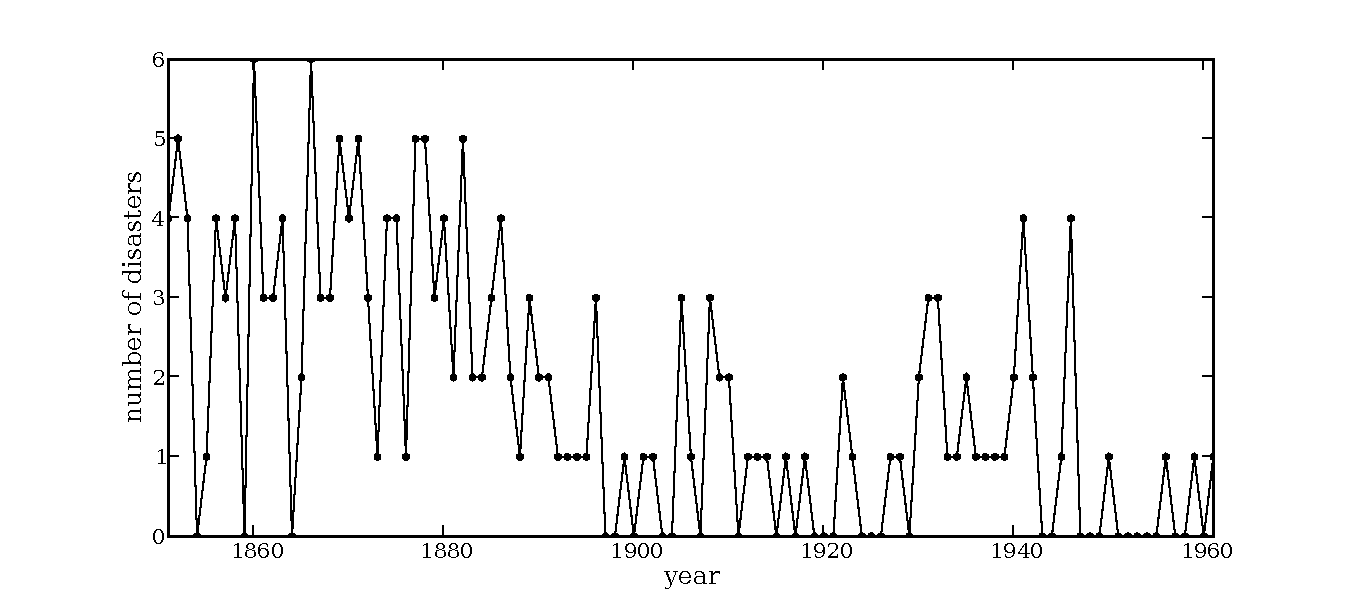
\epsfig{file=disasterts.pdf, width=15cm}
\end{center}
\end{figure}
Occurrences of disasters in the time series is thought to be derived from a Poisson process with a large rate parameter in the early part of the time series, and from one with a smaller rate in the later part. We are interested in locating the change point in the series, which perhaps is related to changes in mining safety regulations.

We represent our conceptual model formally as a statistical model:
\begin{equation}
    \begin{array}{ccc}
        (D_t | s, e, l) \sim \textup{Poisson}\left(r_t\right), & r_t=\left\{\begin{array}{lll}
            e &\textup{if}& t< s\\ l &\textup{if}& t\ge s
            \end{array}\right.,&t\in[t_l,t_h]\\
        s\sim \textup{Discrete Uniform}(t_l, t_h)\\
        e\sim \textup{Exponential}(r_e)\\
        l\sim \textup{Exponential}(r_l)
    \end{array}
    \label{disastermodel}
\end{equation}
The symbols are defined as:
\begin{description}
    \item[$D_t$:] The number of disasters in year $t$.
    \item[$r_t$:] The rate parameter of the Poisson distribution of disasters in year $t$.
    \item[$s$:] The year in which the rate parameter changes (the switchpoint).
    \item[$e$:] The rate parameter before the switchpoint $s$.
    \item[$l$:] The rate parameter after the switchpoint $s$.
    \item[$t_l$, $t_h$:] The lower and upper boundaries of year $t$.
    \item[$r_e$, $r_l$:] The rate parameters of the priors of the early and late rates, respectively.
    %\item[$\beta_e$, $\beta_l$:] Prior parameters (also called hyperparameters).
\end{description}
Because we have defined $D$ by its dependence on $s$, $e$ and $l$, the latter three are known as the `parents' of $D$ and $D$ is called their `child'. Similarly, the parents of $s$ are $t_l$ and $t_h$, and $s$ is the child of $t_l$ and $t_h$.


\section{Two types of variables}

At the model-specification stage (before the data are observed), $D$, $s$, $e$,
$r$ and $l$ are all random variables. Bayesian `random' variables have not
necessarily arisen from a physical random process. The Bayesian interpretation
of probability is \emph{epistemic}, meaning random variable $x$'s probability
distribution $p(x)$ represents our knowledge and uncertainty about $x$'s value
\citep{jaynes}. Candidate values of $x$ for which $p(x)$ is high are
relatively more probable, given what we know. Random variables are represented
in PyMC by the classes \code{Stochastic} and \code{Deterministic}.

The only \code{Deterministic} in the model is $r$. If we knew the values of
$r$'s parents ($s$, $l$ and $e$), we could compute the value of $r$ exactly. A
\code{Deterministic} like $r$ is defined by a mathematical function that returns
its value given values for its parents. \code{Deterministic} variables are
sometimes called the \emph{systemic} part of the model. The nomenclature is a
bit confusing, because these objects usually represent random variables; since
the parents of $r$ are random, $r$ is random also. A more descriptive (though
more awkward) name for this class would be \code{DeterminedByValuesOfParents}.

On the other hand, even if the values of the parents of variables $s$, $D$ (before observing the data), $e$ or $l$ were known, we would still be uncertain of their values. These variables are characterized by probability distributions that express how plausible their candidate values are, given values for their parents. The \code{Stochastic} class represents these variables. A more descriptive name for these objects might be \code{RandomEvenGivenValuesOfParents}.

We can represent model \ref{disastermodel} in a file called
\module{DisasterModel.py} (the actual file can be found in
\file{pymc/examples/}) as follows. First, we import the PyMC and NumPy
namespaces:
\begin{verbatim}
	from pymc import DiscreteUniform, Exponential, deterministic, Poisson, Uniform
	import numpy as np
\end{verbatim}
Notice that from \code{pymc} we have only imported a select few objects that are needed for this particular model, whereas the entire \code{numpy} namespace has been imported, and conveniently given a shorter name. Objects from NumPy are subsequently accessed by prefixing \code{np.} to the name. Either approach is acceptable.

Next, we enter the actual data values into an array:
\begin{verbatim}
	disasters_array =   \
	     numpy.array([ 4, 5, 4, 0, 1, 4, 3, 4, 0, 6, 3, 3, 4, 0, 2, 6,
	                   3, 3, 5, 4, 5, 3, 1, 4, 4, 1, 5, 5, 3, 4, 2, 5,
	                   2, 2, 3, 4, 2, 1, 3, 2, 2, 1, 1, 1, 1, 3, 0, 0,
	                   1, 0, 1, 1, 0, 0, 3, 1, 0, 3, 2, 2, 0, 1, 1, 1,
	                   0, 1, 0, 1, 0, 0, 0, 2, 1, 0, 0, 0, 1, 1, 0, 2,
	                   3, 3, 1, 1, 2, 1, 1, 1, 1, 2, 4, 2, 0, 0, 1, 4,
	                   0, 0, 0, 1, 0, 0, 0, 0, 0, 1, 0, 0, 1, 0, 1])
\end{verbatim}
Note that you don't have to type in this entire array to follow along; the code is available in the source tree, in \file{pymc/examples/DisasterModel.py}.  Next, we create the switchpoint variable $s$:
\begin{verbatim}
	s = DiscreteUniform('s', lower=0, upper=110, doc='Switchpoint[year]')
\end{verbatim}
\code{DiscreteUniform} is a subclass of \code{Stochastic} that represents uniformly-distributed discrete variables. Use of this distribution suggests that we have no preference \emph{a priori} regarding the location of the switchpoint; all values are equally likely. Now we create the exponentially-distributed variables $e$ and $l$ for the early and late Poisson rates, respectively:
\begin{verbatim}
	e = Exponential('e', beta=1)
	l = Exponential('l', beta=1)
\end{verbatim}
Next, we define the variable $r$, which selects the early rate $e$ for times before $s$ and the late rate $l$ for times after $s$. We create $r$ using the \code{deterministic} decorator, which converts the ordinary Python function $r$ into a \code{Deterministic} object.
\begin{verbatim}
	@deterministic(plot=False)
	def r(s=s, e=e, l=l):
		""" Concatenate Poisson means """
	    out = numpy.empty(len(disasters_array))
	    out[:s] = e
	    out[s:] = l
	    return out
\end{verbatim}
The last step is to define the number of disasters $D$. This is a stochastic variable, but unlike $s$, $e$ and $l$ we have observed its value. To express this, we set the argument \code{observed} to \code{True} (it is set to \code{False} by default). This tells PyMC that this object's value should not be changed:
\begin{verbatim}
	D = Poisson('D', mu=r, value=disasters_array, observed=True)
\end{verbatim}

\subsection{Why are data and unknown variables represented by the same
object?}
Since its represented by a \code{Stochastic} object, $D$ is defined by its dependence on its parent $r$ even though its value is fixed. This isn't just a quirk of PyMC's syntax; Bayesian hierarchical notation itself makes no distinction between random variables and data. The reason is simple: to use Bayes' theorem to compute the posterior $p(e,s,l|D)$ of model \ref{disastermodel}, we require the likelihood $p(D|e,s,l)$. Even though $D$'s value is known and fixed, we need to formally assign it a probability distribution as if it were a random variable. Remember, the likelihood and the probability function are essentially the same, except that the former is regarded as a function of the parameters and the latter as a function of the data.

This point can be counterintuitive at first, as many peoples' instinct is to regard data as fixed a priori and unknown variables as dependent on the data. One way to understand this is to think of statistical models like (\ref{disastermodel}) as predictive models for data, or as models of the processes that gave rise to data. Before observing the value of $D$, we could have sampled from its prior predictive distribution $p(D)$ (\emph{i.e.} the marginal distribution of the data) as follows:
\begin{enumerate}
    \item Sample $e$, $s$ and $l$ from their priors.
    \item Sample $D$ conditional on these values.
\end{enumerate}
Even after we observe the value of $D$, we need to use this process model to make inferences about $e$, $s$ and $l$ because its the only information we have about how the variables are related.

% ==================================
% = Does this section really help? =
% ==================================
% \medskip
% To look at the issue another way, we could, in principle, have written a model equivalent to (\ref{disastermodel}) such that $D$ depended on nothing and everything else depended on $D$, for example
% \begin{eqnarray*}
%     s|e,l,D\sim\cdot\\
%     e|l,D\sim\cdot\\
%     l|D\sim\cdot\\
%     D=D_*
% \end{eqnarray*}
%
% In one respect, this would have been more natural because we would have the unknown stochastic variables depending on the data. However, if we could write down that model using standard distributions we could trivially compute and sample from the posterior,
% \begin{eqnarray*}
%     p(s,e,l|D) = p(s|e, l, D) p(e|l, D) p(l|D),
% \end{eqnarray*}
% and we would have no use for MCMC or any other fitting method. Bayesian methods, and statistics in general, are needed when it's feasible to write down the data's dependence on the unknown variables but not vice versa.


\section{Parents and children}

We have above created a PyMC probability model, which is simply a linked collection of variables. To see the nature of the links, import or run \code{DisasterModel.py} and examine $s$'s \code{parents} attribute from the Python prompt:
\begin{verbatim}
   >>> from pymc.examples import DisasterModel
   >>> DisasterModel.s.parents
   {'lower': 0, 'upper': 110}
\end{verbatim}
The \code{parents} dictionary shows us the distributional parameters of $s$, which are constants. Now let's examinine $D$'s parents:
\begin{verbatim}
   >>> DisasterModel.D.parents
   {'mu': <pymc.PyMCObjects.Deterministic 'r' at 0x3e51a70>}
\end{verbatim}
We are using $r$ as a distributional parameter of $D$ (\emph{i.e.} $r$ is $D$'s parent). $D$ internally labels $r$ as \code{mu}, meaning $r$ plays the role of the rate parameter in $D$'s Poisson distribution. Now examine $r$'s \code{children} attribute:
\begin{verbatim}
   >>> DisasterModel.r.children
   set([<pymc.distributions.Poisson 'D' at 0x3e51290>])
\end{verbatim}
Because $D$ considers $r$ its parent, $r$ considers $D$ its child. Unlike \code{parents}, \code{children} is a set (an unordered collection of objects); variables do not associate their children with any particular distributional role. Try examining the \code{parents} and \code{children} attributes of the other parameters in the model.

The following `directed acyclic graph' is a visualization of the parent-child relationships in the model. Unobserved stochastic variables $s$, $e$ and $l$ are open ellipses, observed stochastic variable $D$ is a filled ellipse and deterministic variable $r$ is a triangle. Arrows point from parent to child and display the label that the child assigns to the parent. See section \ref{graphical} for more details.
\begin{figure}[h!]
\begin{center}
   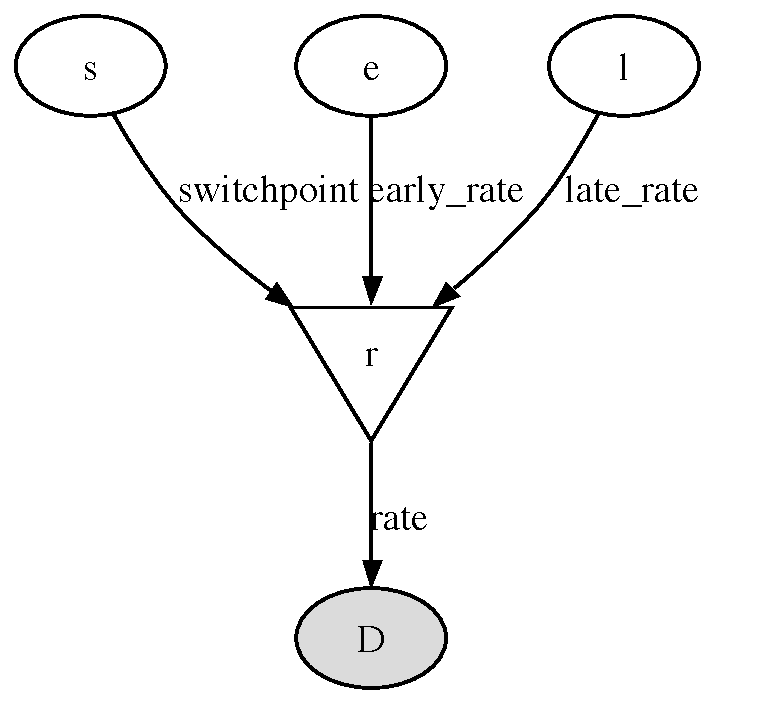
\epsfig{file=DisasterModel2.pdf, width=5cm}
\end{center}
\end{figure}


\begin{center}
\begin{sffamily}
\fbox{\parbox{\admonitionwidth}{
\textbf{\large Objects and names}
\vspace{2mm}
As the examples above have shown, pymc objects need to have a name 
assigned, such as \emph{lower}, \emph{upper} or \emph{e}. These names 
are used for storage and post-processing:
\begin{itemize}
 \item as keys in on-disk databases,
 \item as node labels in model graphs,
 \item as axis labels in plots of traces, 
 \item as table labels in summary statistics. 
\end{itemize}
A model instantiated with variables having identical names raises an
error to avoid name conflicts in the database storing the traces. In
general however, pymc uses references to the objects themselves, not 
their names, to identify variables. 
}}
\end{sffamily}
\end{center}



\section{Variables' values and log-probabilities}
All PyMC variables have an attribute called \code{value} that stores the current value of that variable. Try examining $D$'s value, and you'll see the initial value we provided for it:
\begin{verbatim}
   >>> DisasterModel.D.value
   array([4, 5, 4, 0, 1, 4, 3, 4, 0, 6, 3, 3, 4, 0, 2, 6, 3, 3, 5, 4, 5, 3, 1,
          4, 4, 1, 5, 5, 3, 4, 2, 5, 2, 2, 3, 4, 2, 1, 3, 2, 2, 1, 1, 1, 1, 3,
          0, 0, 1, 0, 1, 1, 0, 0, 3, 1, 0, 3, 2, 2, 0, 1, 1, 1, 0, 1, 0, 1, 0,
          0, 0, 2, 1, 0, 0, 0, 1, 1, 0, 2, 3, 3, 1, 1, 2, 1, 1, 1, 1, 2, 4, 2,
          0, 0, 1, 4, 0, 0, 0, 1, 0, 0, 0, 0, 0, 1, 0, 0, 1, 0, 1])
\end{verbatim}
If you check $e$'s, $s$'s and $l$'s values, you'll see random initial values generated by PyMC:
\begin{verbatim}
   >>> DisasterModel.s.value
   44

   >>> DisasterModel.e.value
   0.33464706250079584

   >>> DisasterModel.l.value
   2.6491936762267811
\end{verbatim}
Of course, since these are \code{Stochastic} elements, your values will be different than these. If you check $r$'s value, you'll see an array whose first $s$ elements are $e$ (here 0.33464706), and whose remaining elements are $l$ (here 2.64919368):
\begin{verbatim}
   >>> DisasterModel.r.value
   array([ 0.33464706,  0.33464706,  0.33464706,  0.33464706,  0.33464706,
           0.33464706,  0.33464706,  0.33464706,  0.33464706,  0.33464706,
           0.33464706,  0.33464706,  0.33464706,  0.33464706,  0.33464706,
           0.33464706,  0.33464706,  0.33464706,  0.33464706,  0.33464706,
           0.33464706,  0.33464706,  0.33464706,  0.33464706,  0.33464706,
           0.33464706,  0.33464706,  0.33464706,  0.33464706,  0.33464706,
           0.33464706,  0.33464706,  0.33464706,  0.33464706,  0.33464706,
           0.33464706,  0.33464706,  0.33464706,  0.33464706,  0.33464706,
           0.33464706,  0.33464706,  0.33464706,  0.33464706,  2.64919368,
           2.64919368,  2.64919368,  2.64919368,  2.64919368,  2.64919368,
           2.64919368,  2.64919368,  2.64919368,  2.64919368,  2.64919368,
           2.64919368,  2.64919368,  2.64919368,  2.64919368,  2.64919368,
           2.64919368,  2.64919368,  2.64919368,  2.64919368,  2.64919368,
           2.64919368,  2.64919368,  2.64919368,  2.64919368,  2.64919368,
           2.64919368,  2.64919368,  2.64919368,  2.64919368,  2.64919368,
           2.64919368,  2.64919368,  2.64919368,  2.64919368,  2.64919368,
           2.64919368,  2.64919368,  2.64919368,  2.64919368,  2.64919368,
           2.64919368,  2.64919368,  2.64919368,  2.64919368,  2.64919368,
           2.64919368,  2.64919368,  2.64919368,  2.64919368,  2.64919368,
           2.64919368,  2.64919368,  2.64919368,  2.64919368,  2.64919368,
           2.64919368,  2.64919368,  2.64919368,  2.64919368,  2.64919368,
           2.64919368,  2.64919368,  2.64919368,  2.64919368,  2.64919368])
\end{verbatim}
To compute its value, $r$ calls the funtion we used to create it, passing in the values of its parents.

\code{Stochastic} objects can evaluate their probability mass or density functions at their current values given the values of their parents. The logarithm of a stochastic object's probability mass or density can be accessed via the \code{logp} attribute. For vector-valued variables like $D$, the \code{logp} attribute returns the sum of the logarithms of the joint probability or density of all elements of the value. Try examining $s$'s and $D$'s log-probabilities and $e$'s and $l$'s log-densities:
\begin{verbatim}
   >>> DisasterModel.s.logp
   -4.7095302013123339

   >>> DisasterModel.D.logp
   -1080.5149888046033

   >>> DisasterModel.e.logp
   -0.33464706250079584

   >>> DisasterModel.l.logp
   -2.6491936762267811
\end{verbatim}
\code{Stochastic} objects need to call an internal function to compute their \code{logp} attributes, as $r$ needed to call an internal function to compute its value. Just as we created $r$ by decorating a function that computes its value, it's possible to create custom \code{Stochastic} objects by decorating functions that compute their log-probabilities or densities (see chapter \ref{chap:modelbuilding}). Users are thus not limited to the set of of statistical distributions provided by PyMC.

\subsection[Using Variables as parents of other Variables]{Using
\code{Variables} as parents of other \code{Variables}}

Let's take a closer look at our definition of $r$:
\begin{verbatim}
	@deterministic(plot=False)
	def r(s=s, e=e, l=l):
	    """ Concatenate Poisson means """
	    out = numpy.empty(len(disasters_array))
	    out[:s] = e
	    out[s:] = l
	    return out
\end{verbatim}
The arguments $s$, $e$ and $l$ are \code{Stochastic} objects, not numbers. Why aren't errors raised when we attempt to slice array \code{out} up to a \code{Stochastic} object?

Whenever a variable is used as a parent for a child variable, PyMC replaces it with its \code{value} attribute when the child's value or log-probability is computed. When $r$'s value is recomputed, \code{s.value} is passed to the function as argument \code{s}. To see the values of the parents of $r$ all together, look at \code{r.parents.value}.

\section{Fitting the model with MCMC}

PyMC provides several objects that fit probability models (linked collections of variables) like ours. The primary such object, \code{MCMC}, fits models with the Markov chain Monte Carlo algorithm \cite{Gamerman:1997tb}. To create an \code{MCMC} object to handle our model, import \module{DisasterModel.py} and use it as an argument for \code{MCMC}:
\begin{verbatim}
   >>> from pymc.examples import DisasterModel
   >>> from pymc import MCMC
   >>> M = MCMC(DisasterModel)
\end{verbatim}
In this case \code{M} will expose variables \code{s}, \code{e}, \code{l}, \code{r} and \code{D} as attributes; that is, \code{M.s} will be the same object as \code{DisasterModel.s}.

To run the sampler, call the MCMC object's \code{isample()} (or \code{sample()}) method with arguments for the number of iterations, burn-in length, and thinning interval (if desired):
\begin{verbatim}
   >>> M.isample(iter=10000, burn=1000, thin=10)
\end{verbatim}
After a few seconds, you should see that sampling has finished normally. The model has been fitted.

\subsection{What does it mean to fit a model?}

`Fitting' a model means characterizing its posterior distribution somehow. In this case, we are trying to represent the posterior $p(s,e,l|D)$ by a set of joint samples from it. To produce these samples, the MCMC sampler randomly updates the values of $s$, $e$ and $l$ according to the Metropolis-Hastings algorithm (\cite{gelman}) for \code{iter}  iterations.

As the number of samples tends to infinity, the MCMC distribution of $s$, $e$
and $l$ converges to the stationary distribution. In other words, their
values can be considered as random draws from the posterior $p(s,e,l|D)$.
PyMC assumes that the \code{burn} parameter specifies a `sufficiently large'
number of iterations for convergence of the algorithm, so it is up to the user
to verify
that this is the case (see chapter \ref{chap:modelchecking}). Consecutive values
sampled from $s$, $e$ and $l$ are necessarily dependent on the previous sample,
since it is a Markov chain. However, MCMC often results in strong
autocorrelation among samples that can result in imprecise posterior inference.
To circumvent this, it is often effective to thin the sample by only retaining
every $k$th sample, where $k$ is an integer value. This thinning interval is
passed to the sampler via the \code{thin} argument.

If you are not sure ahead of time what values to choose for the \code{burn} and \code{thin} parameters, you may want to retain all the MCMC samples, that is to set \code{burn=0} and \code{thin=1}, and then discard the `burnin period' and thin the samples after examining the traces (the series of samples). See \cite{gelman} for general guidance.

\subsection{Accessing the samples}
The output of the MCMC algorithm is a `trace', the sequence of retained
samples for each variable in the model. These traces can be accessed
using the \code{trace(name, chain=-1)} method. For example:
\begin{verbatim}
   >>> M.trace('s')[:]
   array([41, 40, 40, ..., 43, 44, 44])
\end{verbatim}
The trace slice \code{[start:stop:step]} works just like the NumPy array
slice. By default, the returned trace array contains the samples from the
last call to \code{sample}, that is, \code{chain=-1}, but the trace from
previous sampling runs can be retrieved by specifying the correspondent
chain index. To return the trace from all chains, simply use
\code{chain=None}.\footnote{Note that the unknown variables $s$, $e$, $l$ and $r$ will all
accrue samples, but $D$ will not because its value has been observed and is
not updated. Hence $D$ has no trace and calling \code{M.trace('D')[:]} will
raise an error. }

% Alternatively, the trace may be retrieved directly from the variable:
% \begin{verbatim}
%   >>> s.trace()
%   array([41, 40, 40, ..., 43, 44, 44])
% \end{verbatim}

\subsection{Sampling output}
You can examine the marginal posterior of any variable by plotting a histogram of its trace:
\begin{verbatim}
   >>> from pylab import hist, show
   >>> hist(M.trace('l')[:])
   (array([   8,   52,  565, 1624, 2563, 2105, 1292,  488,  258,   45]),
    array([ 0.52721865,  0.60788251,  0.68854637,  0.76921023,  0.84987409,
           0.93053795,  1.01120181,  1.09186567,  1.17252953,  1.25319339]),
    <a list of 10 Patch objects>)
   >>> show()
\end{verbatim}
You should see something like this:
\begin{figure}[h!]
\begin{center}
   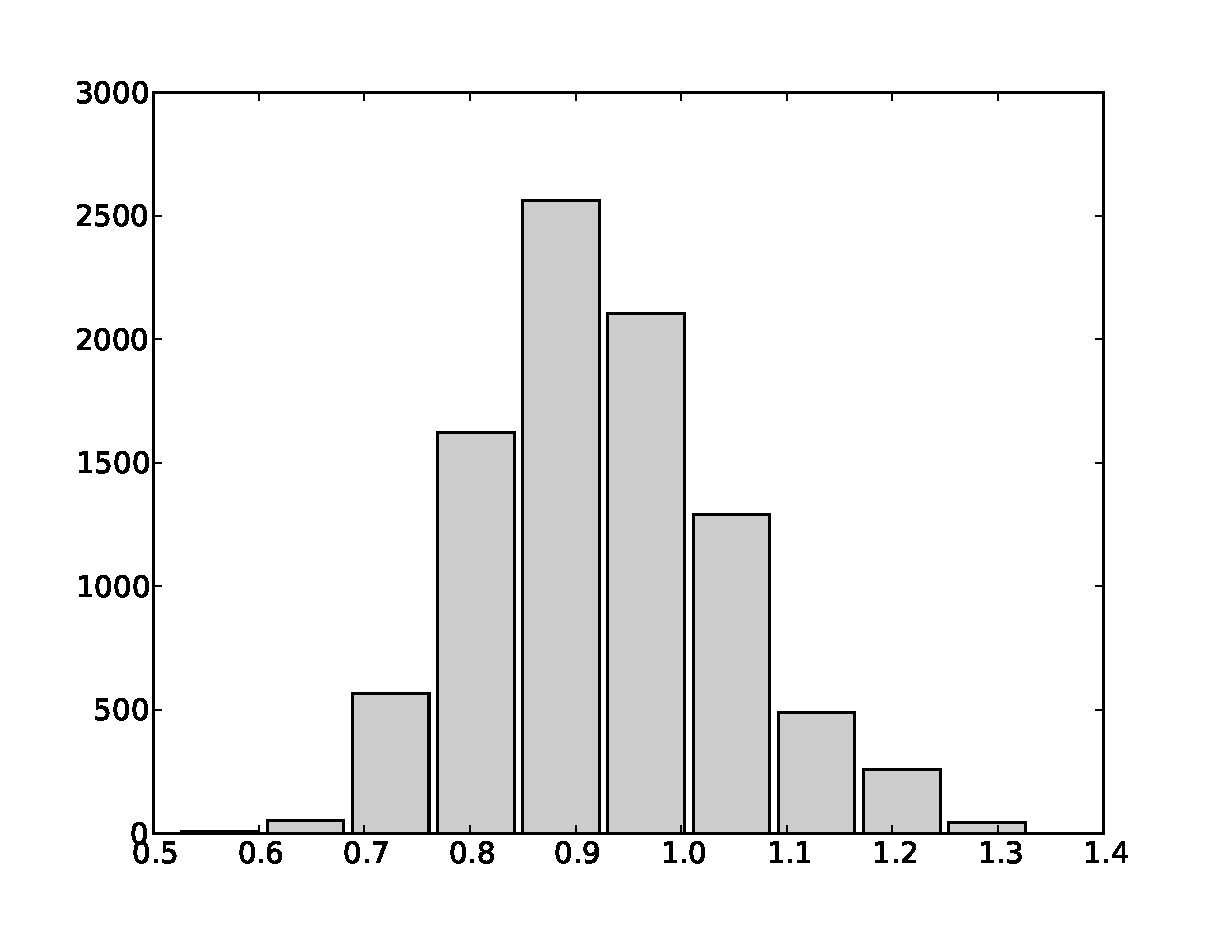
\epsfig{file=ltrace.pdf, width=10cm}
\end{center}
\end{figure}
PyMC has its own plotting functionality, via the optional
\module{matplotlib} module as noted in the installation notes. The
\module{Matplot} module includes a \code{plot} function that takes the
model (or a single parameter) as an argument:
\begin{verbatim}
   >>> from pymc.Matplot import plot
   >>> plot(M)
\end{verbatim}
For each variable in the model, \code{plot} generates a composite figure, such as this one for the switchpoint in the disasters model:
\begin{figure}[h!]
\begin{center}
   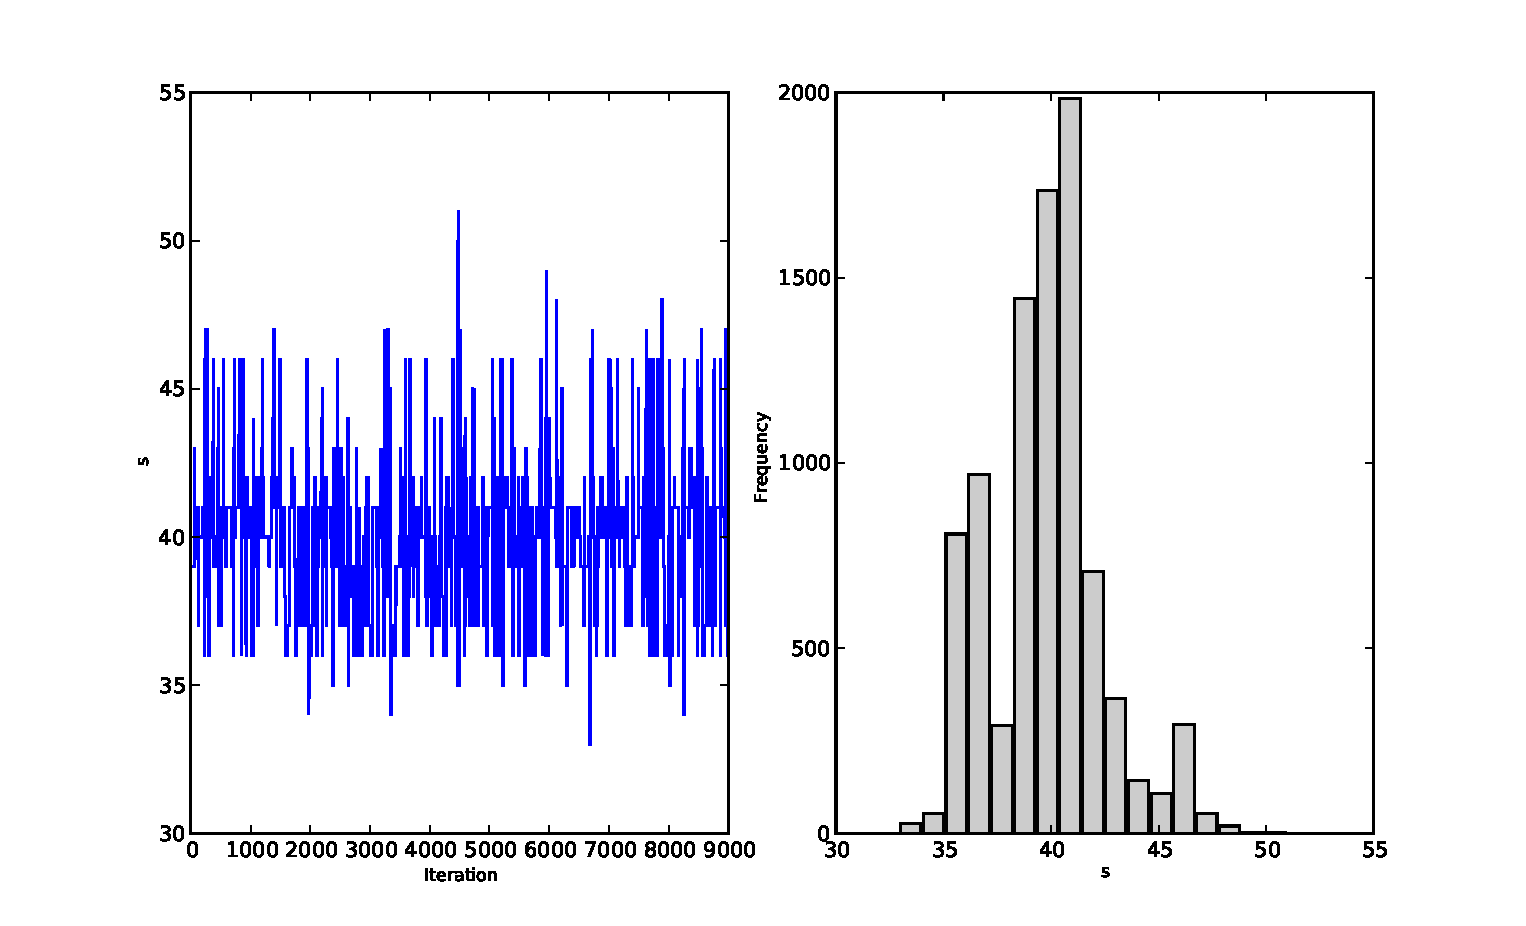
\epsfig{file=spost.pdf, width=15cm}
\end{center}
\end{figure}

The left-hand pane of this figure shows the temporal series of the samples from $s$, while the right-hand pane shows a histogram of the trace. The trace is useful for evaluating and diagnosing the algorithm's performance (see \cite*{gelman}), while the histogram is useful for visualizing the posterior.

For a non-graphical summary of the posterior, simply call \code{M.stats()}.

\hypertarget{missing}{}
\subsection{Imputation of Missing Data} % (fold)
\pdfbookmark[1]{Imputation of Missing Data}{missing}
%\label{subsec:missing_data}

As with most ``textbook examples", the models we have examined so far assume that the associated data are complete. That is, there are no missing values corresponding to any observations in the dataset. However, many real-world datasets contain one or more missing values, usually due to some logistical problem during the data collection process. The easiest way of dealing with observations that contain missing values is simply to exclude them from the analysis. However, this results in loss of information if an excluded observation contains valid values for other quantities, and can bias results. An alternative is to impute the missing values, based on information in the rest of the model.

For example, consider a survey dataset for some wildlife species:

\begin{center}
\begin{tabular}{cccc}
\hline
Count & Site & Observer & Temperature\\
\hline
15 & 1 & 1 & 15\\
10 & 1 & 2 & NA\\
6 & 1 & 1 & 11\\
\hline
\end{tabular}
\end{center}

Each row contains the number of individuals seen during the survey, along with three covariates: the site on which the survey was conducted, the observer that collected the data, and the temperature during the survey. If we are interested in modelling, say, population size as a function of the count and the associated covariates, it is difficult to accommodate the second observation because the temperature is missing (perhaps the thermometer was broken that day). Ignoring this observation will allow us to fit the model, but it wastes information that is contained in the other covariates.

In a Bayesian modelling framework, missing data are accommodated simply by treating them as unknown model parameters. Values for the missing data $\tilde{y}$ are estimated naturally, using the posterior predictive distribution:

\begin{equation}
	p(\tilde{y}|y) = \int p(\tilde{y}|\theta) f(\theta|y) d\theta
\end{equation}

This describes additional data $\tilde{y}$, which may either be considered unobserved data or potential future observations. We can use the posterior predictive distribution to model the likely values of missing data.

Consider the coal mining disasters data introduced previously. Assume that two years of data are missing from the time series; we indicate this in the data array by the use of an arbitrary placeholder value, None.

\begin{verbatim}
x = numpy.array([ 4, 5, 4, 0, 1, 4, 3, 4, 0, 6, 3, 3, 4, 0, 2, 6,
3, 3, 5, 4, 5, 3, 1, 4, 4, 1, 5, 5, 3, 4, 2, 5,
2, 2, 3, 4, 2, 1, 3, None, 2, 1, 1, 1, 1, 3, 0, 0,
1, 0, 1, 1, 0, 0, 3, 1, 0, 3, 2, 2, 0, 1, 1, 1,
0, 1, 0, 1, 0, 0, 0, 2, 1, 0, 0, 0, 1, 1, 0, 2,
3, 3, 1, None, 2, 1, 1, 1, 1, 2, 4, 2, 0, 0, 1, 4,
0, 0, 0, 1, 0, 0, 0, 0, 0, 1, 0, 0, 1, 0, 1])
\end{verbatim}

To estimate these values in PyMC, we generate a masked array. These are specialised NumPy arrays that contain a matching True or False value for each element to indicate if that value should be excluded from any computation. Masked arrays can be generated using NumPy's \code{ma.masked_equal} function:
\begin{verbatim}
>>> masked_data = numpy.ma.masked_equal(x, value=None)
>>> masked_data
masked_array(data = [4 5 4 0 1 4 3 4 0 6 3 3 4 0 2 6 3 3 5 4 5 3 1 4 4 1 5 5 3
 4 2 5 2 2 3 4 2 1 3 -- 2 1 1 1 1 3 0 0 1 0 1 1 0 0 3 1 0 3 2 2 0 1 1 1 0 1 0
 1 0 0 0 2 1 0 0 0 1 1 0 2 3 3 1 -- 2 1 1 1 1 2 4 2 0 0 1 4 0 0 0 1 0 0 0 0 0 1
 0 0 1 0 1],
 mask = [False False False False False False False False False False False False
 False False False False False False False False False False False False
 False False False False False False False False False False False False
 False False False  True False False False False False False False False
 False False False False False False False False False False False False
 False False False False False False False False False False False False
 False False False False False False False False False False False  True
 False False False False False False False False False False False False
 False False False False False False False False False False False False
 False False False],
      fill_value=?)

\end{verbatim}

This masked array, in turn, can then be passed to PyMC's own \code{Impute} function, which replaces the missing values with Stochastic variables of the desired type. For the coal mining disasters problem, recall that disaster events were modelled as Poisson variates:

\begin{verbatim}
	>>> from pymc import Impute
	>>> D = Impute('D', Poisson, masked_data, mu=r)
	>>> D
	[<pymc.distributions.Poisson 'D[0]' at 0x4ba42d0>,
	 <pymc.distributions.Poisson 'D[1]' at 0x4ba4330>,
	 <pymc.distributions.Poisson 'D[2]' at 0x4ba44d0>,
	 <pymc.distributions.Poisson 'D[3]' at 0x4ba45f0>,
	...
	 <pymc.distributions.Poisson 'D[110]' at 0x4ba46d0>]
\end{verbatim}

Here $r$ is an array of means for each year of data, allocated according to the location of the switchpoint. Each element in $D$ is a Poisson Stochastic, irrespective of whether the observation was missing or not. The difference is that actual observations are data Stochastics (\code{observed=True}), while the missing values are non-data Stochastics. The latter are considered unknown, rather than fixed, and therefore estimated by the MCMC algorithm, just as unknown model parameters.

In this example, we have manually generated the masked array for illustration. In practice, the \code{Impute} function will mask arrays automatically, replacing all \code{None} values with Stochastics. Hence, only the original data array needs to be passed.

The entire model looks very similar to the original model:

\begin{verbatim}
	# Switchpoint
	s = DiscreteUniform('s', lower=0, upper=110)
	# Early mean
	e = Exponential('e', beta=1)
	# Late mean
	l = Exponential('l', beta=1)

	@deterministic(plot=False)
	def r(s=s, e=e, l=l):
	    """Allocate appropriate mean to time series"""
	    out = numpy.empty(len(disasters_array))
	    # Early mean prior to switchpoint
	    out[:s] = e
	    # Late mean following switchpoint
	    out[s:] = l
	    return out

	# Where the value of x is None, the value is taken as missing.
	D = Impute('D', Poisson, x, mu=r)
\end{verbatim}

\begin{figure}[ht]
\begin{center}
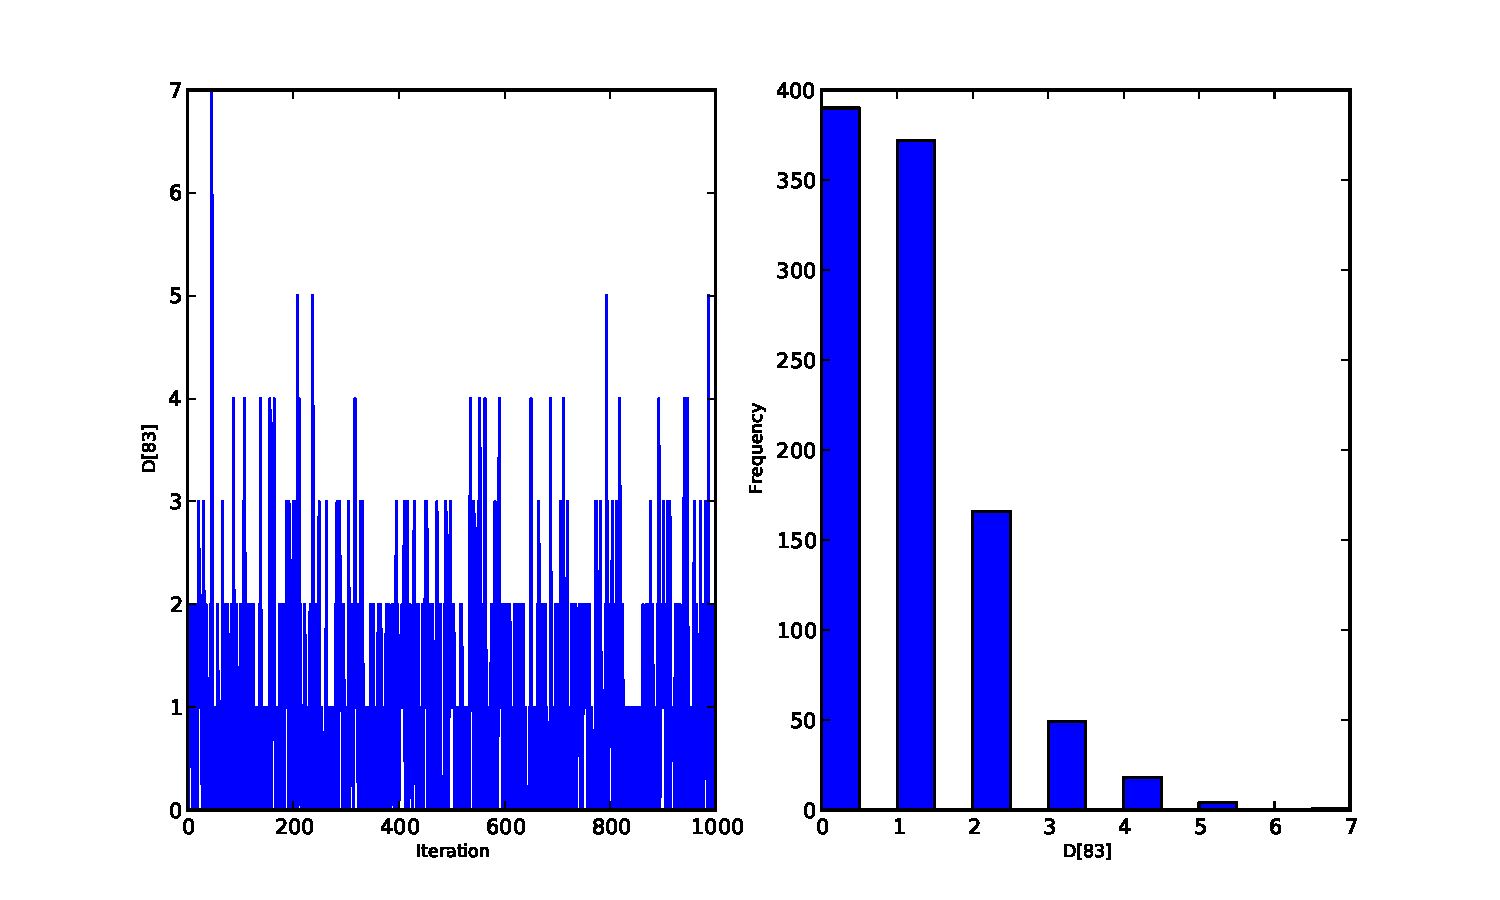
\includegraphics[height=3in]{missing.pdf}
\caption{Trace and posterior distribution of the second missing data point in the example.}
\label{fig:missing}
\end{center}
\end{figure}


The main limitation of this approach for imputation is performance. Because each
element in the data array is modelled by an individual Stochastic, rather than a
single Stochastic for the entire array, the number of nodes in the overall model
increases from 4 to 113. This significantly slows the rate of sampling, due to
the overhead costs associated with iterations over individual nodes.

% section missing_data (end)


\section{Fine-tuning the MCMC algorithm}

MCMC objects handle individual variables via \emph{step methods}, which determine how parameters are updated at each step of the MCMC algorithm. By default, step methods are automatically assigned to variables by PyMC. To see which step methods $M$ is using, look at its \code{step_method_dict} attribute with respect to each parameter:
\begin{verbatim}
   >>> M.step_method_dict[DisasterModel.s]
   [<pymc.StepMethods.DiscreteMetropolis object at 0x3e8cb50>]

   >>> M.step_method_dict[DisasterModel.e]
   [<pymc.StepMethods.Metropolis object at 0x3e8cbb0>]

   >>> M.step_method_dict[DisasterModel.l]
   [<pymc.StepMethods.Metropolis object at 0x3e8ccb0>]
\end{verbatim}
The value of \code{step_method_dict} corresponding to a particular variable is a list of the step methods $M$ is using to handle that variable.

You can force $M$ to use a particular step method by calling \code{M.use_step_method} before telling it to sample. The following call will cause $M$ to handle $l$ with a standard \code{Metropolis} step method, but with proposal standard deviation equal to $2$:
\begin{verbatim}
   >>> from pymc import Metropolis
   M.use_step_method(Metropolis, DisasterModel.l, proposal_sd=2.)
\end{verbatim}

Another step method class, \code{AdaptiveMetropolis}, is better at handling highly-correlated variables. If your model mixes poorly, using \code{AdaptiveMetropolis} is a sensible first thing to try.



\section{Beyond the basics}
That was a brief introduction to basic PyMC usage. Many more topics are covered in the subsequent sections, including:
\begin{itemize}
   \item Class \code{Potential}, another building block for probability models in addition to \code{Stochastic} and \code{Deterministic}
   \item Normal approximations
   \item Using custom probability distributions
   \item Object architecture
   \item Saving traces to the disk, or streaming them to the disk during sampling
   \item Writing your own step methods and fitting algorithms.
\end{itemize}
Also, be sure to check out the documentation for the Gaussian process extension,
which is available on PyMC's
\href{http://code.google.com/p/pymc/downloads/list}{download} page.


\section[Building Models]{Building models}
\label{sec:modelbuilding}
%!TEX root = guide2.0.tex

% \section{Summary}\label{sec:PyMCObjects}
Bayesian inference begins with specification of a probability model relating unknown variables to data. PyMC provides three basic building blocks for Bayesian probability models: \texttt{Stochastic}, \texttt{Deterministic} and \texttt{Potential}. 

A \texttt{Stochastic} object represents a variable whose value is not completely determined by its parents, and a \texttt{Deterministic} object represents a variable that is entirely determined by its parents. In object-oriented programming parlance, \texttt{Stochastic} and \texttt{Deterministic} are subclasses of the \texttt{Variable} class, which is essentially a template for more specific subclasses that are actually implemented in models. The third basic class, representing `factor potentials' (\cite{dawidmarkov,Jordan:2004p5439}), represents an arbitrary log-probability term. \texttt{Potential} and \texttt{Variable}, in turn, are subclasses of \texttt{Node}.

% TODO: Need a better description of what a Potential is. Given the description of Stochastic and Deterministic we have given, its not clear where Potential fits in, as it classifies the world into 2 things -- completely determined by parents and not.

% PyMC also provides container classes for variables to make it easier to program of certain dependency situations, such as when a variable is defined by its dependence on an entire Markov chain.

\medskip
PyMC probability models are simply linked groups of \texttt{Stochastic}, \texttt{Deterministic} and \texttt{Potential} objects. These objects have very limited awareness of the models in which they are embedded and do not themselves possess methods for updating their values in fitting algorithms. Objects responsible for fitting probability models are described in chapter \ref{chap:modelfitting}.
 

\hypertarget{stochastic}{}
\section*{The \texttt{Stochastic} class} \label{stochastic}
\pdfbookmark[0]{The Stochastic class}{stochastic}

A stochastic variable has the following major attributes: 
\begin{description}
    \item[\texttt{value}:] The variable's current value.
    \item[\texttt{logp}:] The log-probability of the variable's current value given the values of its parents.
\end{description}
A stochastic variable can optionally be endowed with a method called \texttt{\bfseries random}, which draws a value for the variable given the values of its parents\footnote{Note that the \texttt{random} method does not provide a Gibbs sample unless the variable has no children.}. Stochastic objects have the following additional attributes that are generally specified automatically, or only specified under particular circumstances:
\begin{description}
    \item[\texttt{parents}:] A dictionary containing the variable's parents. The keys of the dictionary correspond to the names assigned to the variable's parents by the variable, and the values correspond to the actual parents. For example, the keys of $s$'s parents dictionary in model (\ref{disastermodel}) would be \texttt{'t_l'} and \texttt{'t_h'}. Thanks to Python's dynamic typing, the actual parents (\emph{i.e.} the values of the dictionary) may be of any class or type.
    \item[\texttt{children}:] A set containing the variable's children. This set is produced automatically; the user doesn't need to worry about filling it.
    \item[\texttt{extended_parents}:] A set containing all the stochastic variables on which the variable depends either directly or via a sequence of deterministic variables. If the value of any of these variables changes, the variable will need to recompute its log-probability. This set is produced automatically.
    \item[\texttt{extended_children}:] A set containing all the stochastic variables and potentials that depend on the variable either directly or via a sequence of deterministic variables. If the variable's value changes, all of these variables will need to recompute their log-probabilities. This set is produced automatically.
    \item[\texttt{coparents}:] A set containing all the stochastic variables that share extended children with the variable.
    \item[\texttt{moral_neighbors}:] A set containing the union of the variable's extended parents, extended children and coparents, with Potential objects removed.
    \item[\texttt{markov_blanket}:] A set containing self and self's moral neighbors.
    \item[\texttt{isdata}:] A flag (boolean) indicating whether the variable's value has been observed (is fixed).
    \item[\texttt{dtype}:] A Numpy dtype object (such as \texttt{numpy.int}) that specifies the type of the variable's value to fitting methods. If this is \texttt{None} (default) then no type is enforced.
    % \item[\texttt{__name__}:] The name of the variable, should be unique.
    %    \item[\texttt{__doc__}:] The docstring of the variable.
\end{description}

\subsection{Creation of stochastic variables}
There are three main ways to create stochastic variables, called the \textbf{automatic}, \textbf{decorator}, and \textbf{direct} interfaces.

\begin{description}    
    \item[Automatic] Stochastic variables with standard distributions provided by PyMC (see chapter \ref{chap:distributions} ) can be created in a single line using special subclasses of \texttt{Stochastic}. For example, the uniformly-distributed discrete variable $s$ in (\ref{disastermodel}) could be created using the automatic interface as follows:
    \begin{verbatim}
        s = DiscreteUniform('s', 1851, 1962, value=1900)
    \end{verbatim}

    In addition to the classes in chapter \ref{chap:distributions}, \texttt{scipy.stats.distributions}' random variable classes are wrapped as \texttt{Stochastic} subclasses if SciPy is installed. These distributions are in the submodule \texttt{pymc.SciPyDistributions}

    Users can call the class factory \texttt{stochastic_from_dist} to produce \texttt{Stochastic} subclasses of their own from probability distributions not included with PyMC.%  These classes' init methods take the following arguments:
    % \begin{description}
    %     \item[\texttt{name}:] The name of the variable.
    %     \item[\texttt{value}:] An initial value for the variable.
    %     \item[\texttt{parents}:] Keyword arguments specifying the parents of the variable.
    %     \item[\texttt{isdata} (optional)]
    %     \item[\texttt{doc} (optional):] The docstring of the variable.
    %     \item[\texttt{verbose} (optional):] An integer from 0 to 3.
    %     \item[\texttt{trace} (optional):] A boolean indicating whether a trace should be kept for this variable in Monte Carlo fitting methods.
    %     \item[\texttt{cache_depth}:] See section \ref{sec:caching}. 
    % \end{description}
    
    
    \item[Decorator] Uniformly-distributed discrete stochastic variable $s$ in (\ref{disastermodel}) could be created as follows:
    \begin{verbatim}
@stochastic(dtype=int)
def s(value=1900, t_l=1851, t_h=1962):
    """The switchpoint for the rate of disaster occurrence."""
    if value > t_h or value < t_l:
        return -Inf
    else:
        return -log(t_h - t_l + 1) 
    \end{verbatim}
Note that this is a simple Python function, preceded by a Python expression called a \textbf{decorator}, here called \texttt{@stochastic}. Generally, decorators enhance functions with additional properties or functionality. The \texttt{Stochastic} object produced by the \texttt{@stochastic} decorator will evaluate its log-probability using the function \texttt{s}. The \texttt{value} argument, which is required, provides an initial value for the variable. The remaining arguments will be assigned as parents of \texttt{s} (\emph{i.e.} they will populate the \texttt{parents} dictionary).

The \texttt{value} and parents of stochastic variables may be any objects, provided their log-probability functions return a real number (Numpy \texttt{float}). PyMC and SciPy both provide fast implementations of several standard probability distributions that may be helpful for creating custom stochastic variables.

    The decorator \texttt{stochastic} can take several arguments: 
    \begin{itemize}
        \item A flag called \texttt{trace}, which signals to \texttt{MCMC} instances whether an MCMC trace should be kept for the stochastic variable. \texttt{@stochastic(trace = False)} would turn tracing off. Defaults to \texttt{True}.
        \item A flag called \texttt{plot}, which signals to \texttt{MCMC} instances whether summary plots should be produced for this variable. Defaults to \texttt{True}.
        \item An integer-valued argument called \texttt{verbose} that controls the amount of output the variable prints to the screen. The default is $0$, no output; the maximum value is $3$. 
        \item A Numpy datatype called \texttt{dtype}. Decorating a log-probability function with \texttt{@stochastic(dtype=int)} would produce a discrete random variable. Such a variable will cast its value to either an integer or an array of integers. The default dtype is \texttt{float}.
    \end{itemize} 

    The decorator interface has a slightly more complex implementation which allows you to specify a \texttt{random} method for sampling the stochastic variable's value conditional on its parents.
    \begin{verbatim}
@stochastic(dtype=int)
def s(value=1900, t_l=1851, t_h=1962):
    """The switchpoint for the rate of disaster occurrence."""

    def logp(value, t_l, t_h):
        if value > t_h or value < t_l:
            return -Inf
        else:
            return -log(t_h - t_l + 1) 
            
    def random(t_l, t_h):
        return round( (t_l - t_h) * random() ) + t_l

    rseed = 1.
    \end{verbatim}
The stochastic variable again gets its name, docstring and parents from function $s$, but in this case it will evaluate its log-probability using the \texttt{logp} function. The \texttt{random} function will be used when \texttt{s.random()} is called. Note that \texttt{random} doesn't take a \texttt{value} argument, as it generates values itself. The optional \texttt{rseed} variable provides a seed for the random number generator. The stochastic's \texttt{value} argument is optional when a \texttt{random} method is provided; if no initial value is provided, it will be drawn automatically using the \texttt{random} method.

    \item[Direct] It's possible to instantiate \texttt{Stochastic} directly:
\begin{verbatim}
def s_logp(value, t_l, t_h):
    if value > t_h or value < t_l:
        return -Inf
    else:
        return -log(t_h - t_l + 1) 

def s_rand(t_l, t_h):
    return round( (t_l - t_h) * random() ) + t_l

s = Stochastic( logp = s_logp, 
                doc = 'The switchpoint for the rate of disaster occurrence.',
                name = 's', 
                parents = {'t_l': 1851, 't_h': 1962},
                random = s_rand,                 
                trace = True,                 
                value = 1900,
                dtype=int,
                rseed = 1., 
                isdata = False,
                cache_depth = 2,
                plot=True,
                verbose = 0)
\end{verbatim}
Notice that the log-probability and random variate functions are specified externally and passed to \texttt{Stochastic} as arguments. This is a rather awkward way to instantiate a stochastic variable; consequently, such implementations should be rare.

\end{description}


\hypertarget{sub:warning}{}
\subsection*{Don't update stochastic variables' values in-place} \label{sub:warning}
\pdfbookmark[0]{Don't update stochastic variables' values in-place}{sub:warning}

\texttt{Stochastic} objects' values should not be updated in-place. This confuses PyMC's caching scheme and corrupt the process used for accepting or rejecting proposed values in the MCMC algorithm. The only way a stochastic variable's value should be updated is using statements of the following form:
\begin{verbatim}
    A.value = new_value
\end{verbatim}
The following are in-place updates and should \emph{never} be used:
\begin{itemize}
    \item \texttt{A.value += 3}
    \item \texttt{A.value[2,1] = 5}
    \item \texttt{A.value.attribute = new_attribute_value}.
\end{itemize}

This restriction becomes onerous if a step method proposes values for the elements of an array-valued variable separately. In this case, it may be preferable to partition the variable into several variables stored in an array or list.


\hypertarget{data}{}
\section*{Data} \label{data}
\pdfbookmark[0]{Data}{data}

Although the data $D$ is represented by a random variable in the model, we have fixed its value by observing it. Such variables are represented by \texttt{Stochastic} objects whose \texttt{isdata} attribute is set to \texttt{True}. If a stochastic variable's \texttt{isdata} flag is \texttt{True}, its value cannot be changed.

\subsection*{Declaring stochastic variables to be data}

In the short and long interfaces, a \texttt{Stochastic} object's \texttt{isdata} flag can be set to true by stacking a \texttt{@data} decorator on top of the \texttt{@stochastic} decorator:
\begin{verbatim}
@data
@stochastic(dtype=int)
def D(value = count_array, switchpoint = s, early_rate = e, late_rate = l):
    """The observed annual disaster counts."""
    logp = sum(-value[:switchpoint]) + early_rate * log(value[:switchpoint]) \
            - gammaln(early_rate))
    logp += sum(-value[switchpoint:] + late_rate * log(value[switchpoint:]) \
            - gammaln(late_rate))
    return logp
\end{verbatim}
In the automatic and direct interfaces, the \texttt{isdata} argument can be simply set to \texttt{True}.


\hypertarget{deterministic}{}
\section*{The \texttt{Deterministic} class} \label{deterministic}
\pdfbookmark[0]{The Deterministic class}{deterministic}

The \texttt{Deterministic} class represents variables whose values are completely determined by the values of their parents. For example, in model (\ref{disastermodel}), $r$ is a deterministic variable. Recall it was defined by
\begin{eqnarray*}
    r_t=\left\{\begin{array}{ll}
        e & t\le s\\ l & t>s
        \end{array}\right.,
\end{eqnarray*}
so $r$'s value can be computed exactly from the values of its parents $e$, $l$ and $s$.

A deterministic variable's most important attribute is \texttt{\bfseries value}, which gives the current value of the variable given the values of its parents. Like \texttt{Stochastic}'s \texttt{logp} attribute, this attribute is computed on-demand and cached for efficiency.

A Deterministic variable has the following additional attributes:
\begin{description}
    \item[\texttt{parents}:] A dictionary containing the variable's parents. The keys of the dictionary correspond to the names assigned to the variable's parents by the variable, and the values correspond to the actual parents. Thanks to Python's dynamic typing, parents may be of any class or type.
    \item[\texttt{children}:] A set containing the variable's children, which must be nodes. This set is produced automatically; the user doesn't need to worry about filling it.
    % \item[\texttt{__name__}:] The name of the variable, should be unique.
    %     \item[\texttt{__doc__}:] The docstring of the variable.
\end{description}
Deterministic variables have no methods.


\subsection*{Creation of deterministic variables}
Deterministic variables are less complicated than stochastic variables, and have similar \textbf{automatic}, \textbf{decorator}, and \textbf{direct} interfaces:
\begin{description}
   \item[Automatic] A handful of common functions have been wrapped in Deterministic objects. These are brief enough to list:
   \begin{description}
      \item[\texttt{LinearCombination}:] Has two parents $x$ and $y$, both of which must be iterable (\emph{i.e.} vector-valued). This function returns:
      \[
      \sum_i x_i^{\prime} y_i.
      \]
      \item[\texttt{Index}:] Has three parents $x$, $y$ and \texttt{index}. $x$ and $y$ must be iterables, \texttt{index} must be valued as an integer. Index returns the dot product of $x$ and $y$ for the elements specified by \mathttt{index}:
      \[
      x[\mathtt{index}]^T y[\mathtt{index}].
      \]
      \texttt{Index} is useful for implementing dynamic models, in which the parent-child connections change.
      \item[\texttt{Lambda}:] Converts an anonymous function (in Python, called \textbf{lambda functions}) to a \texttt{Deterministic} instance on a single line.
      \item[\texttt{CompletedDirichlet}:] PyMC represents Dirichlet variables of length $k$ by the first $k-1$ elements; since they must sum to 1, the $k^{th}$ element is determined by the others. \texttt{CompletedDirichlet} appends the $k^{th}$ element to the value of its parent $D$.      
      \item[\texttt{Logit}, \texttt{InvLogit}, \texttt{StukelLogit}, \texttt{StukelInvLogit}:] Various common link functions for generalized linear models.
   \end{description}
   It's a good idea to use these classes when feasible, because certain fitting methods (Gibbs step methods in particular) implicitly know how to take them into account.

    \item[Decorator] A deterministic variable can be created via a decorator in a way very similar to \texttt{Stochastic}'s decorator interface:
\begin{verbatim}
@deterministic
def r(switchpoint = s, early_rate = e, late_rate = l):
    """The rate of disaster occurrence."""
    value = zeros(N)
    value[:switchpoint] = early_rate
    value[switchpoint:] = late_rate
    return value
\end{verbatim}
Notice that rather than returning the log-probability, as is the case for \texttt{Stochastic} objects, the function returns the value of the deterministic object, given its parents. This return value may be of any type, as is suitable for the problem at hand. Arguments' keys and values are converted into a parent dictionary as with \texttt{Stochastic}'s short interface. The \texttt{deterministic} decorator can take \texttt{trace} and \texttt{verbose} arguments, like the \texttt{stochastic} decorator.

Of course, since deterministic nodes are not expected to generate random variates, the longer implementation of the decorator interface available to \texttt{Stochastic} objects is not relevant here.

    \item[Direct] Deterministic objects can also be instantiated directly, by passing the evaluation function to the Deterministic class as an argument:
\begin{verbatim}
def r_eval(switchpoint = s, early_rate = e, late_rate = l):
    value = zeros(N)
    value[:switchpoint] = early_rate
    value[switchpoint:] = late_rate
    return value

r = Deterministic(  eval = r_eval, 
                    name = 'r',
                    parents = {'switchpoint': s, 'early_rate': e, 'late_rate': l}),
                    doc = 'The rate of disaster occurrence.',
                    trace = True,
                    verbose = 0,
                    cache_depth = 2)
\end{verbatim}
The \texttt{trace} flag signals to \texttt{Model} whether to keep a trace for the variable, as with stochastic variables.
\end{description}

Note that deterministic variables have no \texttt{isdata} flag. If a deterministic variable's value were known, its parents would be restricted to the inverse image of that value under the deterministic variable's evaluation function. This usage would be extremely difficult to support in general, but it can be implemented for particular applications at the \texttt{StepMethod} level.

\hypertarget{container}{}
\section*{Containers} \label{container}
\pdfbookmark[0]{Containers}{container}

In some situations, such as a state-space model, it would be inconvenient to assign a unique label to each parent of $y$:
\begin{eqnarray*}
    x_0 &\sim& \textup N(0,\tau_x)\\
    x_{i+1}|x_i &\sim& \textup{N}(x_i, \tau_x)\\
    y|x &\sim& \textup N\left(\sum_{i=0}^{N-1}x_i^2,\tau_y\right)\\
	&&i=0,\ldots, N-2
\end{eqnarray*}
Here, $y$ depends on every element of the Markov chain $x$, but we wouldn't want to manually enter $N$ parent labels \texttt{`x_0'}, \texttt{`x_1'}, etc.

This situation can be handled naturally in PyMC:
\begin{verbatim}
x_0 = Normal(`x_0', mu=0, tau=1)

x = [x_0]
last_x = x_0

for i in range(1,N):          
   x_now = Normal(`x_%i' % i, mu=last_x, tau=1)        
   last_x = x_now 
   x.append(x_now)

@data
@stochastic
def y(value = 1, mu = x, tau = 100):
    mu_sum = 0
    for i in range(N):
        mu_sum += mu[i] ** 2
    return normal_like(value, mu_sum, tau)
\end{verbatim}
PyMC automatically wraps list \texttt{x} in an appropriate \texttt{Container} class. The python expression \texttt{`x_\%i' \% i} labels each Normal object in the container with the appropriate index $i$.

Containers, like variables, have an attribute called \texttt{value}. This attribute returns a copy of the (possibly nested) iterable that was passed into the container function, but with each variable inside replaced with its corresponding value. 

Containers can currently be constructed from lists, tuples, dictionaries, Numpy arrays, modules, sets or any object with a \texttt{__dict__} attribute. Variables and non-variables can be freely mixed in these containers, and different types of containers can be nested\footnote{Nodes whose parents are containers make private shallow copies of those containers. This is done for technical reasons rather than to protect users from accidental misuse.}. Containers attempt to behave like the objects they wrap. All containers are subclasses of \texttt{ContainerBase}. 

Containers have the following useful attributes in addition to \texttt{value}:
\begin{itemize}
    \item\texttt{variables}
    \item\texttt{stochastics}
    \item\texttt{potentials}
    \item\texttt{deterministics}
    \item\texttt{data_stochastics}
    \item\texttt{step_methods}.
\end{itemize}
Each of these attributes is a set containing all the objects of each type in a container, and within any containers in the container.


\hypertarget{potential}{}
\section*{The Potential class} \label{potential}
\pdfbookmark[0]{The Potential class}{potential}

% WE PROBABLY NEED TO GIVE A GOOD EXAMPLE OF WHERE A POTENTIAL IS DIFFERENT FROM A DETERMINISTIC;
% THIS PROBABLY WONT BE CLEAR TO EVERYONE. THE KEY DIFFERENCE IS THAT A POTENTIAL IS PART OF THE
% JOINT POSTERIOR, NO?
% 

The joint density corresponding to model (\ref{disastermodel}) can be written as follows:
\begin{eqnarray*}
    p(D,s,l,e) = p(D|s,l,e) p(s) p(l) p(e).
\end{eqnarray*}
Each factor in the joint distribution is a proper, normalized probability distribution for one of the variables conditional on its parents. Such factors are contributed by \texttt{Stochastic} objects.

In some cases, it's nice to be able to modify the joint density by incorporating terms that don't correspond to probabilities of variables conditional on parents, for example:
\begin{eqnarray*}
    p(x_0, x_2, \ldots x_{N-1}) \propto \prod_{i=0}^{N-2} \psi_i(x_i, x_{i+1}).
\end{eqnarray*}
Arbitrary factors such as $\psi$ are contributed by objects of class \texttt{Potential} (\cite{dawidmarkov} and \cite{Jordan:2004p5439} call these terms `factor potentials'). Bayesian hierarchical notation (cf model (\ref{disastermodel})) doesn't accomodate these potentials. They are most useful in cases where there is no natural dependence hierarchy, such as Markov random fields. They are also useful for expressing `soft data' \citep{Christakos:2002p5506}.

Even when there is a definite dependence hierarchy, potentials can provide a useful shorthand. Consider a new example: we have a dataset $t$ consisting of the days on which several marked animals were recaptured. We believe that the probability $S$ that an animal is not recaptured on any given day can be explained by a covariate vector $x$. We model this situation as follows:
\begin{eqnarray*}
    t_i|S_i \sim \textup{Geometric}(S_i), & i=1\ldots N\\
    S_i = \textup{logit}^{-1}(\beta x_i), &i=1\ldots N\\
    \beta\sim \textup{N}(\mu_\beta, V_\beta).
\end{eqnarray*}
So far, so good. Now suppose we have some knowledge of other related experiments and we have a good idea of what $S$ will be before seeing the data. It's not obvious how to work this prior information in, because as we've written the model $S$ is completely determined by $\beta$. There are three options within the strict Bayesian hierarchical framework:
\begin{itemize}
    \item Work the prior information into the prior on $\beta$.
    \item Incorporate the data from the previous experiments explicitly into the model.
    \item Refactor the model so that $S$ is at the bottom of the hierarchy, and assign the prior directly.
\end{itemize}

Factor potentials provide a convenient way to incorporate the prior information without the need for such major modifications. We can simply modify the joint distribution from
\begin{eqnarray*}
    p(t|S(x,\beta)) p(\beta)
\end{eqnarray*}
to
\begin{eqnarray*}
    \gamma(S,a,b) p(t|S(x,\beta)) p(\beta),
\end{eqnarray*}
where $\gamma$ expresses the prior information. It's a good idea to check the induced priors on $S$ and $\beta$ for sanity. This can be done in PyMC by fitting the model with the data $t$ removed.

\bigskip
Potentials have one important attribute, \texttt{\bfseries logp}, the log of their current probability or probability density value given the values of their parents. The only other additional attribute of interest is \texttt{parents}, a dictionary containing the potential's parents. Potentials have no methods. They have no \texttt{trace} attribute, because they are not variables. They cannot serve as parents of variables (for the same reason), so they have no \texttt{children} attribute.


\subsection*{Creation of \texttt{Potentials}}
There are two ways to create potentials:
\begin{description}
    \item[Decorator] A potential can be created via a decorator in a way very similar to \texttt{Deterministic}'s decorator interface:
\begin{verbatim}
@potential
def psi_i(x_lo = x[i], x_hi = x[i+1]):
    """A pair potential"""
    return -(xlo - xhi)**2
\end{verbatim}
The function supplied should return a Numpy \texttt{float}. The \texttt{potential} decorator can take \texttt{verbose} and \texttt{cache_depth} arguments like the \texttt{stochastic} decorator.
    \item[Direct] The same potential could be created directly as follows:
\begin{verbatim}
def psi_i_logp(x_lo = x[i], x_hi = x[i+1]):
    return -(xlo - xhi)**2
        
psi_i = Potential(  logp = psi_i_logp, 
                    name = 'psi_i',
                    parents = {'xlo': x[i], 'xhi': x[i+1]},
                    doc = 'A pair potential',
                    verbose = 0,
                    cache_depth = 2)
\end{verbatim}
\end{description}


\hypertarget{graphical}{}
\section*{Graphing models} \label{graphical}
\pdfbookmark[0]{Graphing models}{graphical}

The function \texttt{graph} draws graphical representations of \texttt{Model} (Chapter \ref{chap:modelfitting}) instances using GraphViz via the Python package PyDot (if they are installed). See \cite{dawidmarkov} and \cite{Jordan:2004p5439} for more discussion of useful information that can be read off of graphical models. Note that these authors do not consider deterministic variables.

The symbol for stochastic variables is an ellipse. Parent-child relationships are indicated by arrows. These arrows point from parent to child and are labeled with the names assigned to the parents by the children. A graphical representation of model \ref{disastermodel} follows:
\begin{center}
    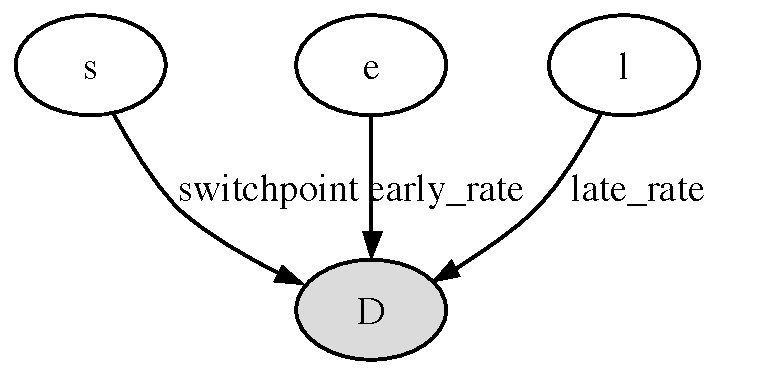
\epsfig{file=DisasterModel.pdf, width=6cm} 
\end{center} 
$D$ is shaded because it is flagged as data.

PyMC's symbol for deterministic variables is a downward-pointing triangle. A graphical representation of model \ref{disastermodel} with $r$ explicit follows:
\begin{center}
    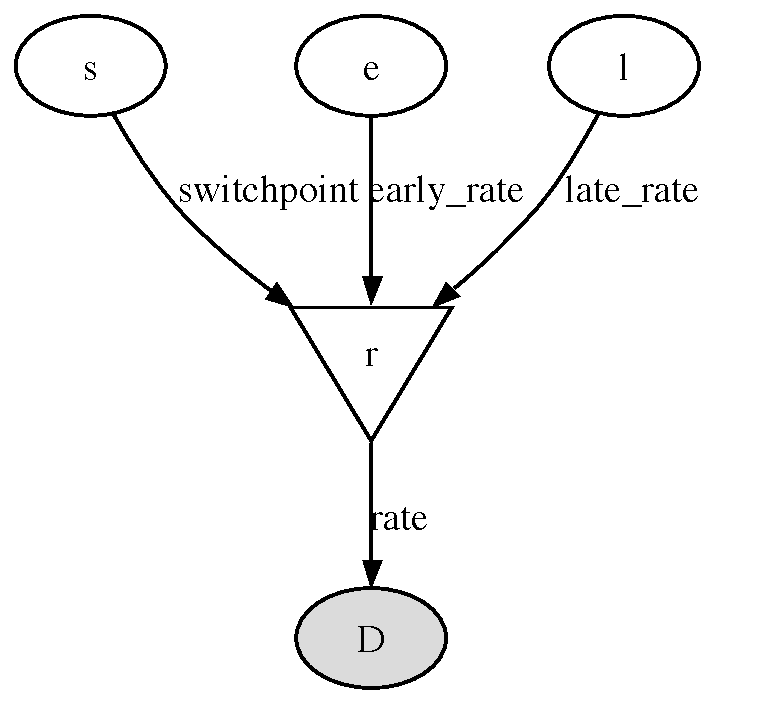
\epsfig{file=DisasterModel2.pdf, width=6cm} 
\end{center}
% Note that if a deterministic variable has more than one child, its parents each inherit all of its children when it is made implicit:
% \begin{center}
%     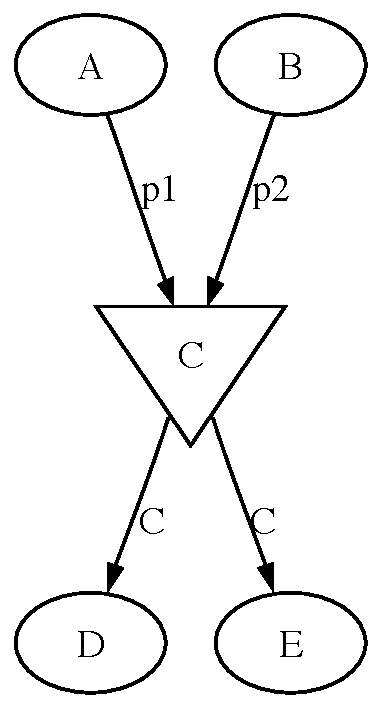
\epsfig{file=DeterministicPreInheritance.pdf, width=3.5cm} $\Rightarrow$ 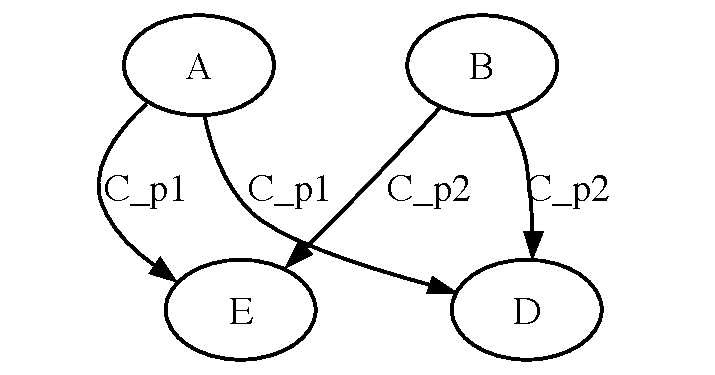
\epsfig{file=DeterministicPostInheritance.pdf, width=5cm}
% \end{center}
% These inherited children can be accessed via the \texttt{extended_children} attributes of the parents.

The symbol for factor potentials is a rectangle:
\begin{center}
    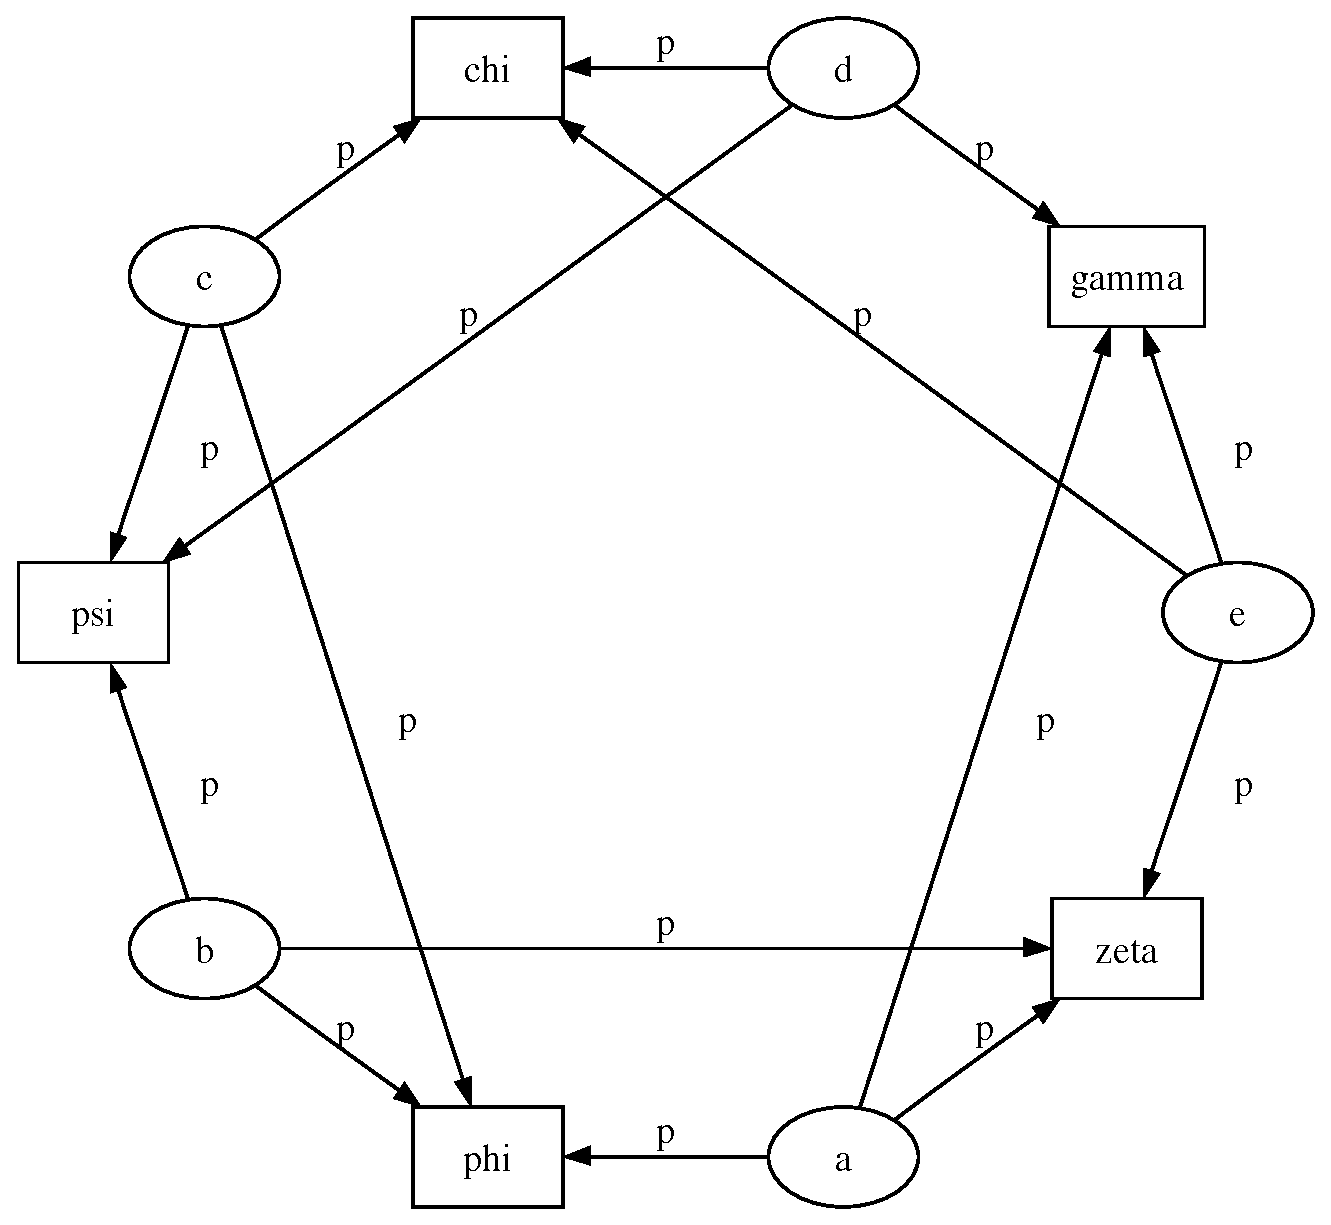
\epsfig{file=PotExample.pdf, width=10cm} 
\end{center}
Factor potentials are usually associated with \emph{undirected} grahical models. In undirected representations, each parent of a potential is connected to every other parent by an undirected edge:
\begin{center}
    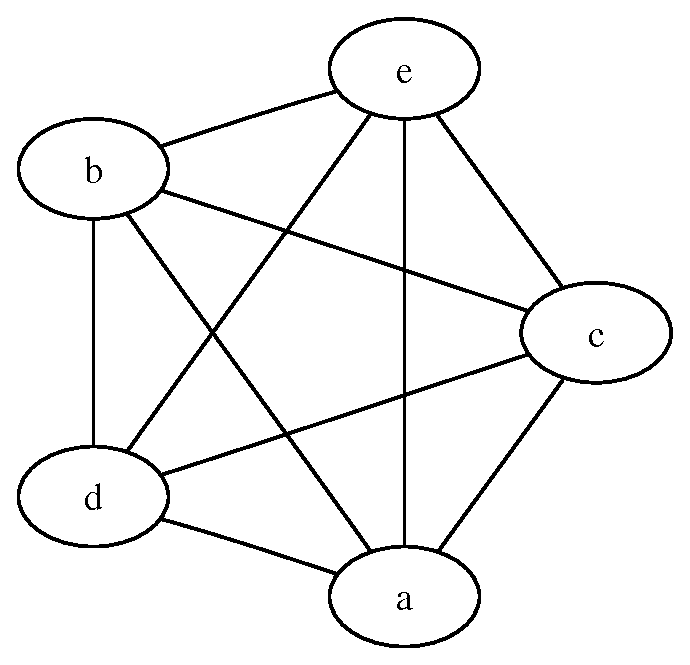
\epsfig{file=PotExampleCollapsed.pdf, width=5cm}
\end{center}

Directed or mixed graphical models can be represented in an undirected form by `moralizing', which is done by the function \texttt{moral_graph}.


\section*{Class \texttt{LazyFunction} and caching}
\label{sec:caching} 

The \texttt{logp} attributes of stochastic variables and potentials and the \texttt{value} attributes of deterministic variables are wrappers for instances of class \texttt{LazyFunction}. Lazy functions are wrappers for ordinary Python functions. A lazy function \texttt{L} could be created from a function \texttt{fun} as follows:
\begin{verbatim}
L = LazyFunction(fun, arguments)
\end{verbatim}
The argument \texttt{arguments} is a dictionary container; \texttt{fun} must accept keyword arguments only. When \texttt{L}'s \texttt{get()} method is called, the return value is the same as the call 
\begin{verbatim}
fun(**arguments.value)
\end{verbatim}
Note that no arguments need to be passed to \texttt{L.get}; lazy functions memorize their arguments.

Before calling \texttt{fun}, \texttt{L} will check the values of \texttt{arguments.variables} against an internal cache. This comparison is done \emph{by reference}, not by value, and this is part of the reason why stochastic variables' values cannot be updated in-place. If \texttt{arguments.variables}' values match a frame of the cache, the corresponding output value is returned and \texttt{fun} is not called. If a call to \texttt{fun} is needed, \texttt{arguments.variables}' values and the return value replace the oldest frame in the cache. The depth of the cache can be set using the optional init argument \texttt{cache_depth}, which defaults to 2.

Caching is helpful in MCMC, because variables' log-probabilities and values tend to be queried multiple times for the same parental value configuration. The default cache depth of 2 turns out to be most useful in Metropolis-Hastings-type algorithms involving proposed values that may be rejected.

Lazy functions are implemented in C using Pyrex, a language for writing Python extensions.

\section[Fitting Models]{Fitting models}
\label{sec:modelfitting}
PyMC probability models are linked collections of nodes. These nodes are only informed by the values of their parents. \code{Deterministic} instances can compute their values given their parents' values, \code{Stochastic} instances can compute their log-probabilities or draw new values, and \code{Potential} instances can compute their log-probabilities. Fitting probability models requires larger-scale coordination and communication.

PyMC provides three objects that fit models:
\begin{itemize}
    \item \code{MCMC}, which coordinates Markov chain Monte Carlo algorithms. The actual work of updating stochastic variables conditional on the rest of the model is done by \code{StepMethod} objects, which are described in this chapter.
    \item \code{MAP}, which computes maximum \emph{a posteriori} estimates.
    \item \code{NormApprox}, which computes the `normal approximation' \citep{gelman}: the joint distribution of all stochastic variables in a model is approximated as normal using local information at the maximum \emph{a posteriori} estimate.
\end{itemize}

All three objects are subclasses of \code{Model}, which is PyMC's base class for fitting methods. \code{MCMC} and \code{NormApprox}, both of which can produce samples from the posterior, are subclasses of \code{Sampler}, which is PyMC's base class for Monte Carlo fitting methods. \code{Sampler} provides a generic sampling loop method and database support for storing large sets of joint samples. These base classes implement some basic methods that are inherited by the three implemented fitting methods, so they are documented at the end of this chapter. %Sampling loops can optionally be run interactively, meaning the user can pause sampling at any time, return to the Python prompt, check progress, and make adjustments.

\section{Creating models} \label{sec:ModelInstantiation}
The first argument to any fitting method's \code{init} method, including that of \code{MCMC}, is called \code{input}. The \code{input} argument can be just about anything; once you have defined the nodes that make up your model, you shouldn't even have to think about how to wrap them in a \code{Model} instance. Some examples of model instantiation using nodes \code{a}, \code{b} and \code{c} follow:
\begin{itemize}
    \item \code{M = Model(set([a,b,c]))}
    \item \code{M = Model(\{`a': a, `d': [b,c]\})} In this case, $M$ will expose $a$ and $d$ as attributes: \code{M.a} will be $a$, and \code{M.d} will be \code{[b,c]}.
    \item \code{M = Model([[a,b],c])}
    \item If file \code{MyModule} contains the definitions of \code{a}, \code{b} and \code{c}:
   \begin{verbatim}
import MyModule
M = Model(MyModule)
    \end{verbatim}
    In this case, $M$ will expose $a$, $b$ and $c$ as attributes.
    \item Using a `model factory' function:
    \begin{verbatim}
def make_model(x):
    a = Exponential('a',.5,beta=x)

    @deterministic
    def b(a=a):
        return 100-a

    @stochastic
    def c(value=.5, a=a, b=b):
        return (value-a)**2/b

    return locals()

M = Model(make_model(3))
    \end{verbatim}
    In this case, $M$ will also expose $a$, $b$ and $c$ as attributes.
\end{itemize}

\hypertarget{model}{}
\subsection[The Model class]{The \code{Model} class} \label{sec:Model}
\pdfbookmark[1]{The Model class}{model}
\code{Model} serves as a container for probability models and as a base class for the classes responsible for model fitting, such as \code{MCMC}. Like any Python class, its properties are inherited by subclasses.

\code{Model}'s init method takes the following arguments:
\begin{description}
    \item[\code{input}:] Some collection of PyMC nodes defining a probability model. These may be stored in a list, set, tuple, dictionary, array, module, or any object with a \code{__dict__} attribute.
    \item[\code{verbose} (optional):] An integer controlling the verbosity of the model's output.
\end{description}

Models' useful methods are:
\begin{description}
    \item[\code{draw_from_prior()}:] Sets all stochastic variables' values to new random values, which would be a sample from the joint distribution if all data and \code{Potential} instances' log-probability functions returned zero. If any stochastic variables lack a \code{random()} method, PyMC will raise an exception.
    \item[\code{seed()}:] Same as \code{draw_from_prior}, but only \code{stochastics} whose \code{rseed} attribute is not \code{None} are changed.
    \item[\code{find_generations():}] Sets the \code{generations} attribute. This attribute is a list whose elements are sets of stochastic variables. The zeroth set has no extended parents in the model, the first set only has extended parents in the zeroth set, and so on.
\end{description}

The helper function \code{graph} produces graphical representations of models \cite[see]{Jordan:2004p5439}.

Models have the following important attributes:
\begin{itemize}
    \item \code{variables}
    \item \code{stochastics}
    \item \code{potentials}
    \item \code{deterministics}
    \item \code{data_stochastics}
    \item \code{step_methods}
    \item \code{value}
\end{itemize}

In addition, models expose each node they contain as an attribute. For instance, if model \code{M} were produced from model (\ref{disastermodel}) \code{M.s} would return the switchpoint variable. It's a good idea to give each variable a unique name if you want to access them this way.


\hypertarget{MAP}{}
\section{Maximum \emph{a posteriori} estimates} \label{sec:MAP}
\pdfbookmark[1]{Maximum a posteriori estimates}{model}

The \code{MAP} class sets all stochastic variables to their maximum \emph{a posteriori} values using functions in SciPy's \code{optimize} package. SciPy must be installed to use it. \code{MAP} can only handle variables whose dtype is \code{float}, so it will not work on model \ref{disastermodel}. To fit the model in \file{examples/gelman_bioassay.py} using \code{MAP}, do the following
\begin{verbatim}
>>> import gelman_bioassay
>>> M = MAP(gelman_bioassay)
>>> M.fit()
\end{verbatim}
This call will cause $M$ to fit the model using Nelder-Mead optimization, which does not require derivatives. The variables in \code{gelman_bioassay} have now been set to their maximum \emph{a posteriori} values:
\begin{verbatim}
>>> M.alpha.value
array(0.8465892309923545)
>>> M.beta.value
array(7.7488499785334168)
\end{verbatim}
In addition, the AIC and BIC of the model are now available:
\begin{verbatim}
>>> M.AIC
7.9648372671389458
>>> M.BIC
6.7374259893787265
\end{verbatim}

\bigskip
\code{MAP} has two useful methods:
\begin{description}
    \item[\code{fit(method ='fmin', iterlim=1000, tol=.0001)}:] The optimization method may be \code{fmin}, \code{fmin_l_bfgs_b}, \code{fmin_ncg}, \code{fmin_cg}, or \code{fmin_powell}. See the documentation of SciPy's \code{optimize} package for the details of these methods. The \code{tol} and \code{iterlim} parameters are passed to the optimization function under the appropriate names.
    \item[\code{revert_to_max()}:] If the values of the constituent stochastic variables change after fitting, this function will reset them to their maximum \emph{a posteriori} values.
\end{description}
If you're going to use an optimization method that requires derivatives, \code{MAP}'s \code{init} method can take additional parameters \code{eps} and \code{diff_order}. \code{diff_order}, which must be an integer, specifies the order of the numerical approximation (see the SciPy function \code{derivative}). The step size for numerical derivatives is controlled by \code{eps}, which may be either a single value or a dictionary of values whose keys are variables (actual objects, not names).

The useful attributes of \code{MAP} are:
\begin{description}
    \item[\code{logp}:] The joint log-probability of the model.
    \item[\code{logp_at_max}:] The maximum joint log-probability of the model.
    % \item[\code{len}:] The total number of elements in all the stochastic variables in the model with \code{observed=False}.
    % \item[\code{data_len}:] The total number number of elements in all the stochastic variables in the model with \code{observed=True}.
    \item[\code{AIC}:] Akaike's information criterion for this model \citep{Akaike:1973aj,Burnham:2002ic}.
    \item[\code{BIC}:] The Bayesian information criterion for this model \citep{Schwarz:1978ud}.
\end{description}

One use of the \code{MAP} class is finding reasonable initial states for MCMC chains. Note that multiple \code{Model} subclasses can handle the same collection of nodes.

\hypertarget{norm-approx}{}
\section{Normal approximations} \label{sec:norm-approx}
\pdfbookmark[1]{Normal approximations}{norm-approx}

The \code{NormApprox} class extends the \code{MAP} class by approximating the posterior covariance of the model using the Fisher information matrix, or the Hessian of the joint log probability at the maximum. To fit the model in \file{examples/gelman_bioassay.py} using \code{NormApprox}, do:
\begin{verbatim}
>>> N = NormApprox(gelman_bioassay)
>>> N.fit()
\end{verbatim}
The approximate joint posterior mean and covariance of the variables are available via the attributes \code{mu} and \code{C}:
\begin{verbatim}
>>> N.mu[N.alpha]
array([ 0.84658923])
>>> N.mu[N.alpha, N.beta]
array([ 0.84658923,  7.74884998])
>>> N.C[N.alpha]
matrix([[ 1.03854093]])
>>> N.C[N.alpha, N.beta]
matrix([[  1.03854093,   3.54601911],
        [  3.54601911,  23.74406919]])
\end{verbatim}
As with \code{MAP}, the variables have been set to their maximum \emph{a posteriori} values (which are also in the \code{mu} attribute) and the AIC and BIC of the model are available.

In addition, it's now possible to generate samples from the posterior as with \code{MCMC}:
\begin{verbatim}
>>> N.sample(100)
>>> N.trace('alpha')[::10]
array([-0.85001278,  1.58982854,  1.0388088 ,  0.07626688,  1.15359581,
       -0.25211939,  1.39264616,  0.22551586,  2.69729987,  1.21722872])
>>> N.trace('beta')[::10]
array([  2.50203663,  14.73815047,  11.32166303,   0.43115426,
        10.1182532 ,   7.4063525 ,  11.58584317,   8.99331152,
        11.04720439,   9.5084239 ])
\end{verbatim}
Any of the database backends can be used (chapter \ref{chap:database}).

\bigskip
In addition to the methods and attributes of \code{MAP}, \code{NormApprox} provides the following methods:
\begin{description}
    \item[\code{sample(iter)}:] Samples from the approximate posterior distribution are drawn and stored.
    \item[\code{isample(iter)}:] An `interactive' version of \code{sample()}: sampling can be paused, returning control to the user.
    \item[\code{draw}:] Sets all variables to random values drawn from the approximate posterior.
\end{description}
It provides the following additional attributes:
\begin{description}
    \item[\code{mu}:] A special dictionary-like object that can be keyed with multiple variables. \code{N.mu[p1, p2, p3]} would return the approximate posterior mean values of stochastic variables \code{p1}, \code{p2} and \code{p3}, ravelled and concatenated to form a vector.
    \item[\code{C}:] Another special dictionary-like object. \code{N.C[p1, p2, p3]} would return the approximate posterior covariance matrix of stochastic variables \code{p1}, \code{p2} and \code{p3}. As with \code{mu}, these variables' values are ravelled and concatenated before their covariance matrix is constructed.
\end{description}

\hypertarget{mcmc}{}
\section[Markov chain Monte Carlo: the MCMC class]{Markov chain Monte
Carlo: the \code{MCMC} class} \label{sec:mcmc}
\pdfbookmark[1]{The MCMC class}{mcmc}

The \code{MCMC} class implements PyMC's core business: producing `traces' for a model's variables which, with careful thinning, can be considered independent joint samples from the posterior. See chapter \ref{chap:tutorial} for an example of basic usage.

\code{MCMC}'s primary job is to create and coordinate a collection of `step methods', each of which is responsible for updating one or more variables. The available step methods are described below. Instructions on how to create your own step method are available in chapter \ref{chap:extending}.

\code{MCMC} provides the following useful methods:
\begin{description}
    \item[\code{sample(iter, burn=0, thin=1, tune\_interval=1000, tune\_throughout=True, save\_interval=None, verbose=0)}:] Runs the MCMC algorithm and produces the traces. The \code{iter} argument controls the total number of MCMC iterations. No tallying will be done during the first \code{burn} iterations; these samples will be forgotten. After this burn-in period, tallying will be done each \code{thin} iterations. Tuning will be done each \code{tune\_interval} iterations. If \code{tune\_throughout=False}, no more tuning will be done after the burnin period. The model state will be saved every \code{save\_interval} iterations, if given.
    \item[\code{isample(iter, burn=0, thin=1, tune\_interval=1000, tune\_throughout=True, save\_interval=None, verbose=0)}:] An interactive version of \code{sample}. The sampling loop may be paused at any time, returning control to the user.
    \item[\code{use_step_method(method, *args, **kwargs)}:] Creates an instance of step method class \code{method} to handle some stochastic variables. The extra arguments are passed to the \code{init} method of \code{method}. Assigning a step method to a variable manually will prevent the \code{MCMC} instance from automatically assigning one. However, you may handle a variable with multiple step methods.
    % \item[\code{assign_step_methods()}:] Assigns step methods to all stochastic variables that do not currently have any. This method is called whenever \code{sample} or \code{isample} is called, but it can be useful to call it directly to see what the default step methods will be.

    % A variable is assigned a step method as follows: each eligible \code{StepMethod} subclass in existence is allowed to inspect the variable in question and determine its competence to handle the variable, on a scale of 0 to 3. An instance of the highest bidder is created to handle the variable.
    \item[\code{goodness()}:] Calculates goodness-of-fit (GOF) statistics according to \cite{Brooks:2000il}.
    \item[\code{save\_state()}:] Saves the current state of the sampler, including all stochastics, to the database. This allows the sampler to be reconstituted at a later time to resume sampling. This is not supported yet for the RDBMS backends, sqlite and mysql.
    \item[\code{restore\_state()}:] Restores the sampler to the state stored in the database.
	 \item[\code{stats()}:] Generate summary statistics for all nodes in the model.
    \item[\code{remember(trace\_index)}:] Set all variables' values from frame \code{trace\_index} in the database.
\end{description}

MCMC samplers' step methods can be accessed via the \code{\textbf{step_method_dict}} attribute. \code{M.step_method_dict[x]} returns a list of the step methods \code{M} will use to handle the stochastic variable \code{x}.

After sampling, the information tallied by a \code{MCMC} instance \code{M}  can be queried via \code{M.db.trace_names}. In addition to the values of variables, tuning information for adaptive step methods is generally tallied. These `traces' can be plotted to verify that tuning has in fact terminated.

You can produce `traces' for arbitrary functions with zero arguments as well. If you issue the command \code{M._funs_to_tally('trace_name') = f} before sampling begins, then each time the model variables' values are tallied \code{f} will be called with no arguments, and the return value will be tallied. After sampling ends you can retrieve the trace as \code{M.trace['trace_name']}

\hypertarget{sampler}{}
\subsection[The Sampler class]{The \code{Sampler} class} \label{sec:Sampler}
\pdfbookmark[1]{The Sampler class}{sampler}
\code{MCMC} is a subclass of a more general class called \code{Sampler}. Samplers fit models with Monte Carlo fitting methods, which characterize the posterior distribution by approximate samples from it. They are initialized as follows: \code{Sampler(input=None, db='ram', name='Sampler', reinit_model=True, calc_deviance=False)}. The \code{input} argument is a module, list, tuple, dictionary, set, or object that contains all elements of the model, the \code{db} argument indicates which database backend should be used to store the samples (see chapter \ref{chap:database}), \code{reinit\_model} is a boolean flag that indicates whether the model should be re-initialised before running, and \code{calc\_deviance} is a boolean flag indicating whether deviance should be calculated for the model at each iteration. Samplers have the following important methods:
\begin{description}
    \item[\code{sample(iter, length=None, verbose=0)}:] Samples from the joint distribution. The \code{iter} argument controls how many times the sampling loop will be run, and the \code{length} argument controls the initial size of the database that will be used to store the samples.
    \item[\code{isample(iter, length=None, verbose=0)}:] The same as \code{sample}, but the sampling is done interactively: you can pause sampling at any point and be returned to the Python prompt to inspect progress and adjust fitting parameters. While sampling is paused, the following methods are useful:
    \begin{description}
        \item[\code{icontinue()}:] Continue interactive sampling.
        \item[\code{halt()}:] Truncate the database and clean up.
    \end{description}
    \item[\code{tally()}:] Write all variables' current values to the database. The actual write operation depends on the specified database backend.
    %\item[\code{draw()}:] Not currently used. In future Monte Carlo fitting methods that aren't MCMC, such as importance samplers, the \code{draw()} method will be responsible for drawing approximate samples from the joint distribution (by setting the values of all the stochastic variables in the model).
    \item[\code{save\_state()}:] Saves the current state of the sampler, including all stochastics, to the database. This allows the sampler to be reconstituted at a later time to resume sampling. This is not supported yet for the RDBMS backends, sqlite and mysql.
    \item[\code{restore\_state()}:] Restores the sampler to the state stored in the database.
	 \item[\code{stats()}:] Generate summary statistics for all nodes in the model.
    \item[\code{remember(trace\_index)}:] Set all variables' values from frame \code{trace\_index} in the database. Note that the \code{trace_index} is different from the current iteration, since not all samples are necessarily saved due to burning and thinning.
\end{description}

In addition, the sampler attribute \code{deviance} is a deterministic variable valued as the model's deviance at its current state.


\hypertarget{step-method}{}
\section{Step methods} \label{sec:stepmethod}
\pdfbookmark[0]{Step methods}{step-method}


Step method objects handle individual stochastic variables, or sometimes groups of them. They are responsible for making the variables they handle take single MCMC steps conditional on the rest of the model. Each subclass of \code{StepMethod} implements a method called \code{step()}, which is called by \code{MCMC}. Step methods with adaptive tuning parameters can optionally implement a method called \code{tune()}, which causes them to assess performance so far and adjust.

The major subclasses of \code{StepMethod} are \code{Metropolis},
\code{AdaptiveMetropolis} and \code{Gibbs}. PyMC provides several flavors of the
basic Metropolis steps, but the Gibbs steps are not ready for use as of the
current release. %However, because it is feasible to write Gibbs step methods
for particular applications, the \code{Gibbs} base class will be documented
here.

\hypertarget{metropolis}{}
\subsection{Metropolis step methods} \label{metropolis}
\pdfbookmark[1]{Metropolis step methods}{metropolis}

\code{Metropolis} and subclasses implement Metropolis-Hastings steps. To tell an \code{MCMC} object $M$ to handle a variable $x$ with a Metropolis step method, you might do the following:
\begin{verbatim}
M.use_step_method(Metropolis, x, proposal_sd=1., proposal_distribution='Normal')
\end{verbatim}

\code{Metropolis} itself handles float-valued variables, and subclasses \code{DiscreteMetropolis} and \code{BinaryMetropolis} handle integer- and boolean-valued variables, respectively. Subclasses of \code{Metropolis} must implement the following methods:
\begin{description}
    \item[\code{propose()}:] Sets the values of the variables handled by the Metropolis step method to proposed values.
    \item[\code{reject()}:] If the Metropolis-Hastings acceptance test fails, this method is called to reset the values of the variables to their values before \code{propose()} was called.
\end{description}
Note that there is no \code{accept()} method; if a proposal is accepted, the variables' values are simply left alone. Subclasses that use proposal distributions other than symmetric random-walk may specify the `Hastings factor' by changing the \code{hastings\_factor} method. See chapter \ref{chap:extending} for an example.

\code{Metropolis}' \texttt{init} method takes the following arguments:
\begin{description}
   \item[\code{stochastic}:] The variable to handle.
   \item[\code{proposal_sd}:] A float or array of floats. This sets the
    default proposal standard deviation if the proposal distribution is normal.
   \item[\code{scale}:] A float, defaulting to 1. If the \code{scale} argument is provided but not \code{proposal_sd}, \code{proposal\_sd} is computed as follows:
   \begin{verbatim}
   if all(self.stochastic.value != 0.):
       self.proposal_sd = ones(shape(self.stochastic.value)) * \
                           abs(self.stochastic.value) * scale
   else:
       self.proposal_sd = ones(shape(self.stochastic.value)) * scale
   \end{verbatim}
   \item[\code{proposal_distribution}:] A string indicating which distribution should be used for proposals. Current options are \code{'Normal'} and \code{'Prior'}. If \code{proposal_distribution=None}, the proposal distribution is chosen automatically. It is set to \code{'Prior'} if the variable has no children and has a random method, and to \code{'Normal'} otherwise.
   \item[\code{verbose}:] An integer. By convention, $0$ indicates minimal output and $2$ indicates maximum verbosity.
\end{description}

Although the \code{proposal\_sd} attribute is fixed at creation, Metropolis step methods adjust this initial value using an attribute called \code{adaptive_scale_factor}. When \code{tune()} is called, the acceptance ratio of the step method is examined and this scale factor is updated accordingly. If the proposal distribution is normal, proposals will have standard deviation \code{self.proposal\_sd * self.adaptive_scale_factor}.

By default, tuning will continue throughout the sampling loop, even after the burnin period is over. This can be changed via the \texttt{tune\_throughout} argument to \texttt{MCMC.sample}. If an adaptive step method's \texttt{tally} flag is set (the default for \texttt{Metropolis}), a trace of its tuning parameters will be kept. If you allow tuning to continue throughout the sampling loop, it is important to verify that the `Diminishing Tuning' condition of \cite{tuning} is satisfied: the amount of tuning should decrease to zero, or tuning should become very infrequent.

If a Metropolis step method handles an array-valued variable, it proposes all elements independently but simultaneously. That is, it decides whether to accept or reject all elements together but it does not attempt to take the posterior correlation between elements into account. The \code{AdaptiveMetropolis} class (see below), on the other hand, does make correlated proposals.

\subsubsection[The AdaptiveMetropolis class]{The
\code{AdaptiveMetropolis} class}
\label{subsec:AM}
The \code{AdaptativeMetropolis} (AM) step method works like a regular Metropolis
step method, with the exception that its variables are block-updated using a
multivariate jump distribution whose covariance is tuned during sampling.
Although the chain is non-Markovian, it has correct ergodic properties (see
\cite{Haario:2001lr}).

To tell an \code{MCMC} object $M$ to handle variables $x$, $y$ and $z$ with an
\code{AdaptiveMetropolis} instance, you might do the following:
\begin{verbatim}
   M.use_step_method(AdaptiveMetropolis, [x,y,z], \
                      scales={'x':1, 'y':2, 'z':.5}, delay=10000)
\end{verbatim}

\code{AdaptativeMetropolis}' init method takes the following arguments:
% cov=None, delay=1000, scales=None, interval=200, greedy=True,verbose=0
\begin{description}
   \item[\code{stochastics}:] The stochastic variables to handle. These will be
updated jointly.
   \item[\code{cov} (optional):] An initial covariance matrix. Defaults to the
identity matrix, adjusted according to the \code{scales} argument.
   \item[\code{delay} (optional):] The number of iterations to delay before
computing the empirical covariance matrix.
   \item[\code{scales} (optional):] The initial covariance matrix will be
diagonal, and its diagonal elements will be set to \code{scales} times the
stochastics' values, squared.
   \item[\code{interval} (optional):] The number of iterations between updates
of the covariance matrix. Defaults to 1000.
   \item[\code{greedy} (optional):] If \code{True}, only accepted jumps will be
counted toward the delay before the covariance is first computed. Defaults to
\code{True}.
   \item[\code{verbose}:] An integer from 0 to 3 controlling the verbosity of
the step method's printed output.
\end{description}

In this algorithm, jumps are proposed from a multivariate normal
distribution with covariance matrix $\Sigma$. The algorithm first iterates
until \code{delay} samples have been drawn (if \code{greedy} is true, until
\code{delay} jumps have been accepted). At this point, $\Sigma$ is given
the value of the empirical covariance of the trace so far and sampling
resumes. The covariance is then updated each \code{interval}
iterations throughout the entire sampling run\footnote{The covariance is
estimated recursively from the previous value and the last \code{interval}
samples, instead of computing it each time from the entire trace.}. It is
this constant adaptation of the proposal distribution that makes the chain
non-Markovian.

\subsubsection[The DiscreteMetropolis class]{The
\code{DiscreteMetropolis} class}
This class is just like \code{Metropolis}, but specialized to handle
\code{Stochastic} instances with dtype \code{int}. The jump proposal
distribution can either be \code{'Normal'}, \code{'Prior'} or \code{'Poisson'}.
In the normal case, the proposed value is drawn from a normal distribution
centered at the current value and then rounded to the
nearest integer. In the Poisson case, the proposed value is obtained by adding
or substracting (with equal probability) a random value drawn from a Poisson
distribution.

\subsubsection[The BinaryMetropolis class]{The
\code{BinaryMetropolis} class}
This class is specialized to handle \code{Stochastic} instances with dtype
\code{bool}.

For array-valued variables, \code{BinaryMetropolis} can be set to propose from
the prior by passing in \code{dist="Prior"}. Otherwise, the argument
\code{p_jump} of the init method specifies how probable a change is. Like
\code{Metropolis}' attribute \code{proposal_sd}, \code{p_jump} is tuned
throughout the sampling loop via \code{adaptive_scale_factor}.

For scalar-valued variables, \code{BinaryMetropolis} behaves like a Gibbs
sampler, since this requires no additional expense. The \code{p_jump} and
\code{adaptive_scale_factor} parameters are not used in this case.

% ==========================================================
% = We can uncomment this when we actually release them... =
% ==========================================================
% \hypertarget{gibbs}{}
% \subsection{Gibbs step methods} \label{gibbs}
% \pdfbookmark[1]{Gibbs step methods}{gibbs}
%
% Conjugate submodels (see \cite{gelman}) can be handled by Gibbs step methods rather than the default Metropolis methods. Gibbs step methods are Metropolis methods whose acceptance rate is always 1. They can be convenient because they relieve the user from having to worry about tuning the acceptance rate, but they can be computationally expensive. When variables are highly dependent on one another, better mixing can often be obtained by using \code{AdaptiveMetropolis} even when Gibbs step methods are available.
%
% Alpha versions of Gibbs step methods handling the following conjugate submodels are available in the \code{sandbox} module, but they are not recommended and will not be assigned automatically:
% \begin{itemize}
%     \item Gamma-Gamma
%     \item Gamma-Exponential
%     \item Gamma-Poisson
%     \item Gamma-Normal
%     \item Beta-Geometric
%     \item Beta-Binomial
%     \item Wishart-Multivariate Normal (represented by the \code{MvNormal} class, which is parameterized by precision)
%     \item Dirichlet-Multinomial.
%     \item Normal-Normal (or Normal-MvNormal, etc.) (requires \code{cvxopt}, \href{http://abel.ee.ucla.edu/cvxopt}{http://abel.ee.ucla.edu/cvxopt} )
% \end{itemize}
% However, if you implement a custom Gibbs step method, subclassing the \code{Gibbs} class will ensure interopera
%
% Gibbs step methods have the following class attributes:
% \begin{itemize}
%     \item \code{child_class}: The step method can handle variables whose children are all of this class. \code{GammaNormal.child_class} is \code{Normal}, for example.
%     \item \code{parent_label}: The target variable's children must refer to it by this label. \code{GammaNormal.parent_label} is \code{'mu'}.
%     \item \code{target_class}: The target variable should be of this class for the submodel to be fully conjugate. \code{GammaNormal.target_class} is \code{Gamma}.
%     \item \code{linear_OK}: A flag indicating whether the variable's children can depend on a multiple of the variable. Such multiples must be implemented via the \code{Deterministic} subclass \code{LinearCombination}.
% \end{itemize}
%
% A Gibbs step method can handle variables that are not of their target class, as long as all their children are of the appropriate class. If this is the case, the step method's \code{conjugate} attribute will be set to \code{False} and its acceptance rate will no longer be 1.
%
% Gibbs step methods are easy to use manually. To tell an \code{MCMC}
% object $M$ to handle a variable $x$ using the \code{GammaNormal} class,
% simply use the call
% \begin{verbatim}
%     M.use_step_method(GammaNormal, x)
% \end{verbatim}
%
% To indicate a general preference for Gibbs step methods vs. Metropolis step methods, set the following global integer values:
% \begin{itemize}
%     \item \code{pymc.conjugate_Gibbs_competence}: Applicable Gibbs step methods' competence functions will return this value for variables that are not of their target classes. The default value is 0, meaning that these methods will never be assigned automatically. Set this value to 3 to ensure that Gibbs step methods are always be assigned to conjugate submodels, or to 1.5 to set their priorities between those of \code{Metropolis} and \code{AdaptiveMetropolis}.
%     \item \code{pymc.nonconjugate_Gibbs_competence}: Applicable Gibbs step methods' competence functions will return this value for variables that are of their target classes. The default value is 0, meaning that these methods are never assigned automatically.
% \end{itemize}
%

\subsection{Granularity of step methods: one-at-a-time vs. block updating}
\label{subsec:granularity}
There is currently no way for a stochastic variable to compute individual terms of its log-probability; it is computed all together. This means that updating the elements of a array-valued variable individually would be inefficient, so all existing step methods update array-valued variables together, in a block update.

To update an array-valued variable's elements individually, simply break it up into an array of scalar-valued variables. Instead of this:
\begin{verbatim}
A = Normal('A', value=zeros(100), mu=0., tau=1.)
\end{verbatim}
do this:
\begin{verbatim}
A = [Normal('A_%i'%i, value=0., mu=0., tau=1.) for i in xrange(100)]
\end{verbatim}
An individual step method will be assigned to each element of \code{A} in the latter case, and the elements will be updated individually. Note that \code{A} can be broken up into larger blocks if desired.

\subsection{Automatic assignment of step methods}
Every step method subclass (including user-defined ones) that does not require any \texttt{init} arguments other than the stochastic variable to be handled adds itself to a list called \code{StepMethodRegistry} in the PyMC namespace. If a stochastic variable in an \code{MCMC} object has not been explicitly assigned a step method, each class in \code{StepMethodRegistry} is allowed to examine the variable.

To do so, each step method implements a class method called \code{competence(stochastic)}, whose only argument is a single stochastic variable. These methods return values from 0 to 3; 0 meaning the step method cannot safely handle the variable and 3 meaning it will most likely perform well for variables like this. The \code{MCMC} object assigns the step method that returns the highest competence value to each of its stochastic variables.



\section[Sampling Results]{Saving and managing sampling results}
\label{sec:database}


A typical MCMC run will generate thousands of samples, and some application requires well over 100000 iterations. Keeping all this information in memory can badly strain the performances of PyMC, and users will find their other applications slowing down. Moreover, we generally wish to store all or part of the sampled data for future use. However, there are dozens of different solutions to store data, and each user has his own preference based on previous experience, performance, compatibility, etc. To cover as many user cases as possible, PyMC proposes a database backend. That is, instead of hardcoding data management in the Sampler or Deterministic class, we ask that each stoch is provided with a set of methods taking care of tallying values, and eventually, returning them. PyMC provides a couple of backends for popular data management tools , but users have the possibility to code their own custom made backend, and let Sampler use it seamlessly.


%FIXME This table runs over the page.
\begin{longtable}[c]{|p{0.12\locallinewidth}|p{0.60\locallinewidth}|p{0.20\locallinewidth}|}
\caption{Description of database backends available in PyMC 2.0.}\\
\hline
\textbf{
Backend
} & \textbf{
Description
} & \textbf{
Dependencies
} \\
\hline
\endhead

no{\_}trace
 & 
Do not tally samples. Very efficient, mostly used
for testing purposes.
 & 
None
 \\
\hline

RAM
 & 
Store samples in memory. Efficient for small to
medium size samples.
 & 
None
 \\
\hline

pickle
 & 
Store samples in memory, then dump them in a
pickle file.
 & 
Cpickle
 \\
\hline

sqlite
 & 
Store samples in a sqlite database.
 & 
sqlite3
 \\
\hline

mysql
 & 
Store samples in a mysql database.
 & 
MySQLdb
 \\
\hline

txt
 & 
Store samples in memory, then dump them in a txt
file.
 & 
None
 \\
\hline

hdf5
 & 
Store samples in the HDF5 format.
 & 
pytables2.0
 \\
\hline
\end{longtable}

Backends are selected at Sampler instantiation through the db keyword:
\begin{quote}{\ttfamily \raggedright \noindent
S~=~Sampler(DisasterSampler,~db='sqlite')
}\end{quote}

Another possibility is to instantiate a Database, then pass it to Sampler:
\begin{quote}{\ttfamily \raggedright \noindent
DB~=~database.sqlite.Database(filename='test')~\\
S~=~Sampler(DisasterSampler,~db=DB)
}\end{quote}

This calling mechanism allows user to pass arguments to the Database, instead
of relying on the defaults. For databases that provide a load function, it also
allows user to open an existing database and restart interrupted computations:
\begin{quote}{\ttfamily \raggedright \noindent
DB~=~database.pickle.load('results.pickle')~\\
S~=~Sampler(DisasterSampler,~db=DB)
}\end{quote}


%___________________________________________________________________________

\hypertarget{use-of-trace-methods}{}
\pdfbookmark[0]{Use of trace methods}{use-of-trace-methods}
\section*{Use of trace methods}
\label{use-of-trace-methods}

From the user perpective, the only method that really matters is the gettrace()
method (equivalent to trace.{\_}{\_}call{\_}{\_}). This method returns the values tallied during sampling. So for
instance:
\begin{quote}{\ttfamily \raggedright \noindent
S~=~Sampler(DisasterModel,~db='ram')~\\
S.sample(30000,10000,2)
}\end{quote}

Will tally in memory every other sample, creating arrays of 15000 elements. To
fetch the last 10000 values of stoch \titlereference{e} say, we would type:
\begin{quote}{\ttfamily \raggedright \noindent
S.e.trace(burn=5000)
}\end{quote}


%___________________________________________________________________________

\hypertarget{backend-requirements}{}
\pdfbookmark[0]{Backend requirements}{backend-requirements}
\section*{Backend requirements}
\label{backend-requirements}

Each backend must define minimally two classes: Database and Trace. The Database
class is responsible for opening files, connecting to databases, assigning
tallyable nodes a Trace instance and calling its methods. Optionnaly,
the Database class can provide methods to save and return the state of the
sampler. This is useful for very long computations liable to be stopped then
restarted at a later time.
The Trace class defines several methods to tally and return the trace of nodes.

The basic framework of those classes is displayed in \href{PyMC2/database/base.py}{database/base.py}. Each
backend subclasses the base clases.

For more information about individual backends, refer to the \href{docs/API.pdf}{API} documentation.

\

\section[Model Checking]{Model checking and diagnostics}
\label{sec:modelchecking}
\hypertarget{convergence}{}
\pdfbookmark[0]{Convergence Diagnostics}{convergence}
\section{Convergence Diagnostics} % (fold)
%\label{sec:convergence_diagnostics}

Valid inferences from sequences of MCMC samples are based on the assumption that the samples are derived from the true posterior distribution of interest. Theory guarantees this condition as the number of iterations approaches infinity. It is important, therefore, to determine the minimum number of samples required to ensure a reasonable approximation to the target posterior density. Unfortunately, no universal threshold exists across all problems, so convergence must be assessed independently each time MCMC estimation is performed. The procedures for verifying convergence are collectively known as convergence diagnostics.

One approach to analyzing convergence is analytical, whereby the variance of the sample at different sections of the chain are compared to that of the limiting distribution. These methods use distance metrics to analyze convergence, or place theoretical bounds on the sample variance, and though they are promising, they are generally difficult to use and are not prominent in the MCMC literature. More common is a statistical approach to assessing convergence. With this approach, rather than considering the properties of the theoretical target distribution, only the statistical properties of the observed chain are analyzed. Reliance on the sample alone restricts such convergence criteria to heuristics; that is, convergence cannot be guaranteed. Although evidence for lack of convergence using statistical convergence diagnostics will correctly imply lack of convergence in the chain, the absence of such evidence will not \emph{guarantee} convergence in the chain. Nevertheless, negative results for one or more criteria will provide some measure of assurance to most users that their sample will provide valid inferences.

For most simple models, convergence will occur quickly, sometimes within a the first several hundred iterations, after which all remaining samples of the chain may be used to calculate posterior quantities. For many more complex models, convergence requires a significantly longer burn-in period; sometimes  orders of magnitude more samples are needed. Frequently, lack of convergence will be caused by poor mixing (Figure \ref{fig:mix}). Recall that \emph{mixing} refers to the degree to which the Markov chain explores the support of the posterior distribution. Poor mixing may stem from inappropriate proposals (if one is using the Metropolis-Hastings sampler) or from attempting to estimate models with highly correlated variables.

\begin{figure}[ht]
\begin{center}
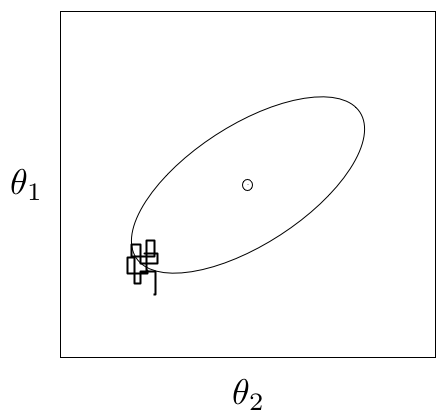
\includegraphics[height=3in]{poormixing.png}
\caption{An example of a poorly-mixing sample in two dimensions. Notice that the chain is trapped in a region of low probability relative to the mean (dot) and variance (oval) of the true posterior quantity.}
\label{fig:mix}
\end{center}
\end{figure}

\subsection{Informal Methods}

The most straightforward approach for assessing convergence is based on
simply plotting and inspecting traces and histograms of the observed MCMC
sample. If the trace of values for each of the stochastics exhibits asymptotic
behaviour\footnote{Asymptotic behaviour implies that the variance and the
mean value of the sample stays relatively constant over some arbitrary
period.} over the last $m$ iterations, this may be satisfactory evidence
for convergence. A similar approach involves plotting a histogram for every
set of $k$ iterations (perhaps 50-100) beyond some burn in threshold $n$;
if the histograms are not visibly different among the sample intervals,
this is reasonable evidence for convergence. Note that such diagnostics
should be carried out for each stochastic estimated by the MCMC algorithm,
because convergent behaviour by one variable does not imply evidence for
convergence for other variables in the analysis. An extension of this approach
can be taken when multiple parallel chains are run, rather than just a
single, long chain. In this case, the final values of $c$ chains run for
$n$ iterations are plotted in a histogram; just as above, this is repeated
every $k$ iterations thereafter, and the histograms of the endpoints are
plotted again and compared to the previous histogram. This is repeated
until consecutive histograms are indistinguishable.

\begin{figure}[h]
\begin{center}
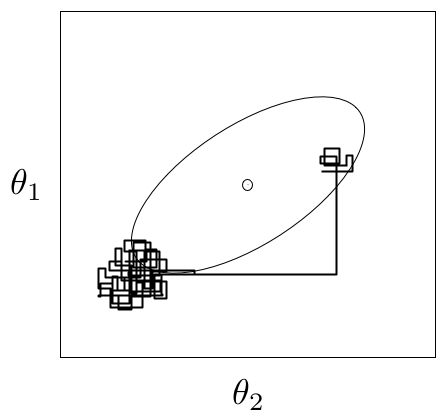
\includegraphics[height=3in]{metastable.png}
\caption{An example of metastability in a two-dimensional parameter space. The chain appears to be stable in one region of the parameter space for an extended period, then unpredictably jumps to another region of the space.}
\label{fig:metas}
\end{center}
\end{figure}

Another \emph{ad hoc} method for detecting convergence is to examine the traces of several MCMC chains initialized with different starting values. Overlaying these traces on the same set of axes should (if convergence has occurred) show each chain tending toward the same equilibrium value, with approximately the same variance. Recall that the tendency for some Markov chains to converge to the true (unknown) value from diverse initial values is called \emph{ergodicity}. This property is guaranteed by the reversible chains constructed using MCMC, and should be observable using this technique. Again, however, this approach is only a heuristic method, and cannot always detect lack of convergence, even though chains may appear ergodic.

A principal reason that evidence from informal techniques cannot guarantee convergence is a phenomenon called metastability. Chains may appear to have converged to the true equilibrium value, displaying excellent qualities by any of the methods described above. However, after some period of stability around this value, the chain may suddenly move to another region of the parameter space (Figure \ref{fig:metas}). This period of metastability can sometimes be very long, and therefore escape detection by these convergence diagnostics. Unfortunately, there is no statistical technique available for detecting metastability.

\subsection{Formal Methods}

Along with the \emph{ad hoc} techniques described above, a number of more formal methods exist which are prevalent in the literature. These are considered more formal because they are based on existing statistical methods, such as time series analysis.

PyMC currently includes two formal convergence diagnostic methods. The first, proposed by \citet{Geweke:1992gm}, is a time-series approach that compares the mean and variance of segments from the beginning and end of a single chain.
\begin{equation}
z = \frac{\bar{\theta}_a - \bar{\theta}_b}{\sqrt{Var(\theta_a) + Var(\theta_b)}}
\end{equation}
where $a$ is the early interval and $b$ the late interval. If the z-scores (theoretically distributed as standard normal variates) of these two segments are similar, it can provide evidence for convergence. PyMC calculates z-scores of the difference between various initial segments along the chain, and the last 50\% of the remaining chain. If the chain has converged, the majority of points should fall within 2 standard deviations of zero.

Diagnostic z-scores can be obtained by calling the \code{geweke} function. It accepts either (1) a single trace, (2) a dictionary of traces, (3) a Node object, or (4) an entire Model object.

\subsubsection*{Method Usage}
\begin{verbatim}
geweke(x, first=0.1, last=0.5, intervals=20)
\end{verbatim}
\begin{itemize}

\item \verb=x=: The object that is or contains the output trace(s).

\item \verb=first= (optional): First portion of chain to be used in Geweke diagnostic. Defaults to 0.1 (i.e. first 10\% of chain).

\item \verb=last= (optional): Last portion of chain to be used in Geweke diagnostic. Defaults to 0.5 (i.e. last 50\% of chain).

\item \verb=intervals= (optional): Number of sub-chains to analyze. Defaults to 20.
\end{itemize}

The resulting scores are best interpreted graphically, using the \code{geweke_plot} function. This displays the scores in series, in relation to the 2 standard deviation boundaries around zero. Hence, it is easy to see departures from the standard normal assumption.

\begin{figure}[ht]
\begin{center}
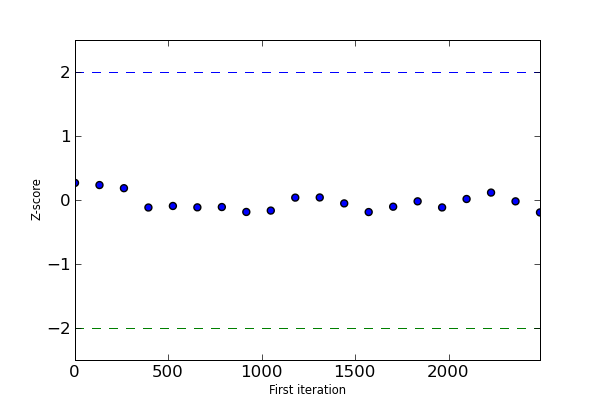
\includegraphics[height=3in]{geweke.png}
\caption{Sample plot of Geweke z-scores for a variable using \textbf{geweke_plot}. The occurrence of the scores well within 2 standard deviations of zero gives does not indicate lack of convergence.}
\label{fig:geweke}
\end{center}
\end{figure}

\code{geweke_plot} takes either a single set of scores, or a dictionary of scores (output by \code{geweke} when an entire Sampler is passed) as its argument:

\subsubsection*{Method Usage}
\begin{verbatim}
def geweke_plot(data, name='geweke', format='png', suffix='-diagnostic', \
                path='./', fontmap = {1:10, 2:8, 3:6, 4:5, 5:4}, verbose=1)
\end{verbatim}
\begin{itemize}

\item \verb=data=: The object that contains the Geweke scores. Can be a list (one set) or a dictionary (multiple sets).

\item \verb=name= (optional): Name used for output files. For multiple scores, the dictionary keys are used as names.

\item \verb=format= (optional): Graphic output file format (defaults to \emph{png}).

\item \verb=suffix= (optional): Suffix to filename (defaults to \emph{-diagnostic})

\item \verb=path= (optional): The path for output graphics (defaults to working directory).

\item \verb=fontmap= (optional): Dictionary containing the font map for the labels of the graphic.

\item \verb=verbose= (optional): Verbosity level for output (defaults to 1).
\end{itemize}

To illustrate, consider a model \code{my_model} that is used to instantiate a MCMC sampler. The sampler is then run for a given number of iterations:
\begin{verbatim}
	>>> S = pymc.MCMC(my_model)
	>>> S.sample(10000, burn=5000)
\end{verbatim}
It is easiest simply to pass the entire sampler \code{S} the \code{geweke} function:
\begin{verbatim}
	>>> scores = pymc.geweke(S, intervals=20)
	>>> pymc.Matplot.geweke_plot(scores)
\end{verbatim}
Alternatively, individual stochastics within \code{S} can be analyzed for convergence:
\begin{verbatim}
	>>> trace = S.alpha.trace()
	>>> alpha_scores = pymc.geweke(trace, 'alpha', intervals=20)
	>>> pymc.Matplot.geweke_plot(alpha_scores)
\end{verbatim}

The second diagnostic provided by PyMC is the \citet{raftery} procedure. This approach estimates the number of iterations required to reach convergence, along with the number of burn-in samples to be discarded and the appropriate thinning interval. A separate estimate of both quantities can be obtained for each variable in a given model.

As the criterion for determining convergence, the Raftery and Lewis approach uses the accuracy of estimation of a user-specified quantile. For example, we may want to estimate the quantile $q=0.975$ to within $r=0.005$ with probability $s=0.95$. In other words,

\begin{equation}
	Pr(|\hat{q}-q| \le r) = s
\end{equation}

From any sample of $\theta$, one can construct a binary chain:

\begin{equation}
	Z^{(j)} = I(\theta^{(j)} \le u_q)
\end{equation}

where $u_q$ is the quantile value and $I$ is the indicator function. While $\{\theta^{(j)}\}$ is a Markov chain, $\{Z^{(j)}\}$ is not necessarily so. In any case, the serial dependency among $Z^{(j)}$ decreases as the thinning interval $k$ increases. A value of $k$ is chosen to be the smallest value such that the first order Markov chain is preferable to the second order Markov chain.

This thinned sample is used to determine number of burn-in samples. This is done by comparing the remaining samples from burn-in intervals of increasing length to the limiting distribution of the chain. An appropriate value is one for which the truncated sample's distribution is within $\epsilon$ (arbitrarily small) of the limiting distribution. See \citet{raftery} or \citet{Gamerman:1997tb} for computational details. Estimates for sample size tend to be conservative.

This diagnostic is best used on a short pilot run of a particular model, and the results used to parameterize a subsequent sample that is to be used for inference.


\subsubsection*{Method Usage}
\begin{verbatim}
raftery_lewis(x, q, r, s=.95, epsilon=.001, verbose=1)
\end{verbatim}
\begin{itemize}

	\item \verb=x=: The object that contains the Geweke scores. Can be a list (one set) or a dictionary (multiple sets).

    \item \verb=q=: Desired quantile to be estimated.

    \item \verb=r=: Desired accuracy for quantile.

    \item \verb=s=(optional): Probability of attaining the requested accuracy (defaults to 0.95).

    \item \verb=epsilon= (optional) : Half width of the tolerance interval required for the q-quantile (defaults to 0.001).

    \item \verb=verbose= (optional) : Verbosity level for output (defaults to 1).
\end{itemize}

The code for \code{raftery_lewis} is based on the FORTRAN program \emph{gibbsit}, which was written by Steven Lewis.

For example, consider again a sampler \code{S} run for some model \code{my_model}:
\begin{verbatim}
	>>> S = pymc.MCMC(my_model)
	>>> S.sample(10000, burn=5000)
\end{verbatim}
One can pass either the entire sampler \code{S} or any stochastic within \code{S} to the \code{raftery_lewis} function, along with suitable arguments. Here, we have chosen $q=0.025$ (the lower limit of the equal-tailed 95\% interval) and error $r=0.01$:
\begin{verbatim}
	>>> pymc.raftery_lewis(S, q=0.025, r=0.01)
\end{verbatim}
This yields diagnostics as follows for each stochastic of \code{S}, as well as a dictionary containing the diagnostic quantities:

\begin{verbatim}
	========================
	Raftery-Lewis Diagnostic
	========================

	937 iterations required (assuming independence) to achieve 0.01 accuracy 
	with 95 percent probability.

	Thinning factor of 1 required to produce a first-order Markov chain.

	39 iterations to be discarded at the beginning of the simulation (burn-in).

	11380 subsequent iterations required.

	Thinning factor of 11 required to produce an independence chain.
\end{verbatim}

Additional convergence diagnostics are available in the
\href{http://lib.stat.cmu.edu/R/CRAN/}{R statistical package}, via the
\href{http://www-fis.iarc.fr/coda/}{CODA module}. PyMC includes a method
\code{coda} for exporting model traces in a format that may be
directly read by CODA.

\subsubsection*{Method Usage}
\begin{verbatim}
pymc.utils.coda(pymc_object)
\end{verbatim}
\begin{itemize}

\item \verb=pymc_object=: The PyMC sampler for which output is desired.

\end{itemize}
Calling \verb=coda= yields a file containing raw trace values (suffix
\verb=.out=) and a file containing indices to the trace values (suffix
\verb=.ind=).

% section convergence_diagnostics (end)

\hypertarget{autocorrelation}{}
\pdfbookmark[0]{Autocorrelation Plots}{autocorrelation}
\section{Autocorrelation Plots} % (fold)
%\label{sec:autocorrelation_plots}

Samples from MCMC algorithms are ususally autocorrelated, due partly to the
inherent Markovian dependence structure. The degree of autocorrelation can
be quantified using the autocorrelation function:
\begin{eqnarray*}
    \rho_k &=& \frac{\mbox{Cov}(X_t,
X_{t+k})}{\sqrt{\mbox{Var}(X_t)\mbox{Var}(X_{t+k})}} \\
            &=& \frac{E[(X_t - \theta)(X_{t+k} - \theta)]}{\sqrt{E[(X_t -
\theta)^2] E[(X_{t+k} - \theta)^2]}}
\end{eqnarray*}
PyMC includes a function for plotting the autocorrelation function for each
stochastics in the sampler (Figure \ref{fig:autocorr}). This allows users
to examine the relationship among successive samples within sampled chains.
Significant autocorrelation suggests that chains require thinning prior to
use of the posterior statistics for inference.

\begin{figure}[h]
        \begin{center}
        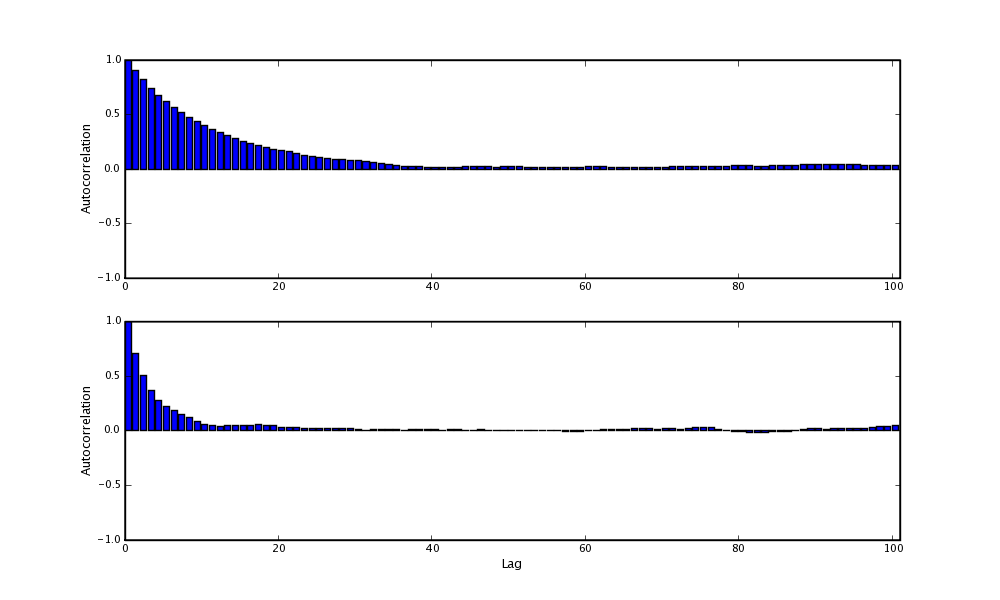
\includegraphics[scale=0.4]{autocorr.png}
    \end{center}
    \caption{Sample autocorrelation plots for two Poisson variables from
coal mining disasters example model.}
    \label{fig:autocorr}
\end{figure}

\begin{verbatim}
autocorrelation(data, name, maxlag=100, format='png', suffix='-acf',
path='./', fontmap = {1:10, 2:8, 3:6, 4:5, 5:4}, verbose=1)
\end{verbatim}
\begin{itemize}
	\item \verb=data=: The object that is or contains the output
trace(s).

	\item \verb=name=: Name used for output files.

	\item \verb=maxlag=: The highest lag interval for which
autocorrelation is calculated.

	\item \verb=format= (optional): Graphic output file format
(defaults to \emph{png}).

	\item \verb=suffix= (optional): Suffix to filename (defaults to
\emph{-diagnostic})

	\item \verb=path= (optional): The path for output graphics
(defaults to working directory).

	\item \verb=fontmap= (optional): Dictionary containing the font map
for the labels of the graphic.

	\item \verb=verbose= (optional): Verbosity level for output
(defaults to 1).
\end{itemize}

% section autocorrelation_plots (end)

\hypertarget{gof}{}
\pdfbookmark[0]{Goodness of Fit}{gof}
\section{Goodness of Fit} % (fold)
%\label{sec:goodness_of_fit}

Checking for model convergence is only the first step in the evaluation of MCMC model outputs. It is possible for an entirely unsuitable model to converge, so additional steps are needed to ensure that the estimated model adequately fits the data. One intuitive way for evaluating model fit is to compare model predictions with actual observations. In other words, the fitted model can be used to simulate data, and the distribution of the simulated data should resemble the distribution of the actual data.

Fortunately, simulating data from the model is a natural component of the Bayesian modelling framework. Recall, from the discussion on imputation of missing data, the posterior predictive distribution:

\begin{equation}
	p(\tilde{y}|y) = \int p(\tilde{y}|\theta) f(\theta|y) d\theta
\end{equation}

Here, $\tilde{y}$ represents some hypothetical new data that would be expected, taking into account the posterior uncertainty in the model parameters. Sampling from the posterior predictive distribution is easy in PyMC. The code looks identical to the corresponding data stochastic, with two modifications: (1) the node should be specified as deterministic and (2) the statistical likelihoods should be replaced by random number generators. As an example, consider the Poisson data likelihood of the coal mining disasters example:
\begin{verbatim}
	@pm.stochastic(observed=True, dtype=int)
	def disasters(  value = disasters_array,
	                early_mean = early_mean,
	                late_mean = late_mean,
	                switchpoint = switchpoint):
	    """Annual occurences of coal mining disasters."""
	    return pm.poisson_like(value[:switchpoint],early_mean) +
	 pm.poisson_like(value[switchpoint:],late_mean)
\end{verbatim}
This is a mixture of Poisson processes, one with a higher early mean and another with a lower late mean. Here is the corresponding sample from the posterior predictive distribution:
\begin{verbatim}
	@pm.deterministic
	def disasters_sim(early_mean = early_mean,
	                late_mean = late_mean,
	                switchpoint = switchpoint):
	    """Coal mining disasters sampled from the posterior predictive distribution"""
	    return concatenate( (pm.rpoisson(early_mean, size=switchpoint),
	 pm.rpoisson(late_mean, size=n-switchpoint)))
\end{verbatim}
Notice that \code{@pm.stochastic} has been replaced with \code{@pm.deterministic} and \code{pm.poisson_like} with \code{pm.rpoisson}. The simulated values from each of the Poisson processes are concatenated together before returning them.

The degree to which simulated data correspond to observations can be evaluated in at least two ways. First, these quantities can simply be compared visually. This allows for a qualitative comparison of model-based replicates and observations. If there is poor fit, the true value of the data may appear in the tails of the histogram of replicated data, while a good fit will tend to show the true data in high-probability regions of the posterior predictive distribution (Figure~\ref{fig:gof}).

\begin{figure}[h]
        \begin{center}
        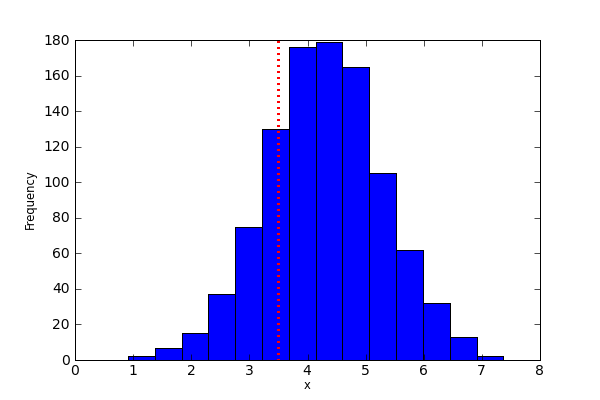
\includegraphics[height=3in]{gof.png}
    \end{center}
    \caption{Data sampled from the posterior predictive distribution of a model for some observation \textbf{x}. The true value of \textbf{x} is shown by the dotted red line.}
    \label{fig:gof}
\end{figure}

The Matplot package in PyMC provides an easy way of producing such plots, via the \code{gof_plot} function. To illustrate, consider a single data point \code{x} and an array of values \code{x_sim} sampled from the posterior predictive distribution. The histogram is generated by calling:

\begin{verbatim}
	pm.Matplot.gof_plot(x_sim, x, name='x')
\end{verbatim}

A second approach for evaluating goodness of fit using samples from the posterior predictive distribution involves the use of a statistical criterion. For example, the Bayesian p-value \citep{Gelman:1996gp} uses a discrepancy measure that quantifies the difference between data (observed or simulated) and the expected value, conditional on some model. One such discrepancy measure is the Freeman-Tukey statistic \citep{Brooks:2000il}:

\begin{equation}
	D(x|\theta) = \sum_j (\sqrt{x_j}-\sqrt{e_j})^2
\end{equation}

Model fit is assessed by comparing the discrepancies from observed data to those from simulated data. On average, we expect the difference between them to be zero; hence, the Bayesian p-value is simply the proportion of simulated discrepancies that are larger than their corresponding observed discrepancies:

\begin{equation}
	p = Pr[ D(\text{sim}) > D(\text{obs}) ]
\end{equation}

If $p$ is very large (e.g. $>0.975$) or very small (e.g. $<0.025$) this implies that the model is not consistent with the data, and thus is evidence of lack of fit. Graphically, data and simulated discrepancies plotted together should be clustered along a 45 degree line passing through the origin, as shown in Figure~\ref{fig:deviate}.

\begin{figure}[h]
        \begin{center}
        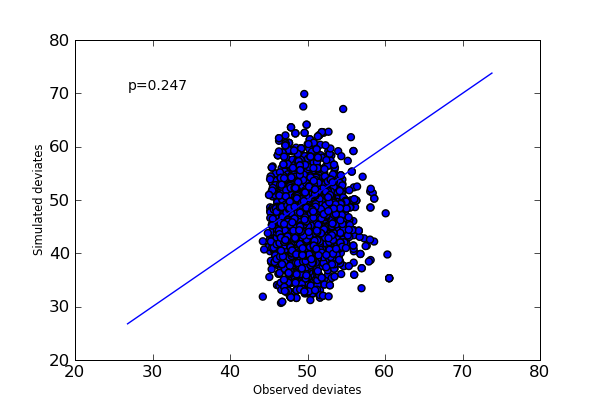
\includegraphics[height=3in]{deviates.png}
    \end{center}
    \caption{Plot of deviates of observed and simulated data from expected values. The cluster of points symmetrically about the 45 degree line (and the reported p-value) suggests acceptable fit for the modeled parameter.}
    \label{fig:deviate}
\end{figure}

The \code{discrepancy} function in the \code{utils} package can be used to generate discrepancy statistics from arrays of data, simulated values, and expected values:

\begin{verbatim}
	D = pm.utils.discrepancy(observed, simulated, expected)
\end{verbatim}

A call to this function returns two arrays of discrepancy values, which can be passed to the \code{discrepancy_plot} function in the Matplot module to generate a scatter plot, and if desired, a p-value:

\begin{verbatim}
	pm.Matplot.discrepancy_plot(D, name='D', report_p=True)
\end{verbatim}

Additional optional arguments for \code{discrepancy_plot} are identical to other PyMC plotting functions.

% section goodness_of_fit (end)


\section[Extending PyMC]{Extending PyMC}
\label{sec:extending}
\bigskip
Note that you don't need to understand this section; any covariance function that satisfies the calling convention described in section \ref{subsub:cov} will work. The \texttt{cov_funs} module is convenient, but it is admittedly complicated.

\bigskip
The \class{covariance_function_bundle} class includes versions of each covariance function using several different distance metrics. For example, the Euclidean version of the Mat\`ern covariance function is \texttt{matern.euclidean} and the Gaussian covariance function in geographic coordinates (in radians) is \texttt{gaussian.geo_rad}.

In addition, it has two attributes that are included for extensibility: the \texttt{raw} attribute, which exposes the basic Fortran implementation of each function, and \texttt{add_distance_metric} method, which combines the \texttt{raw} attribute with distance metrics. This section will describe these attributes in more detail.

Class \texttt{covariance_function_bundle}'s init method takes three arguments:
\begin{description}
	\item[\texttt{cov_fun_name}] The name of the covariance function.
	\item[\texttt{cov_fun_module}] The name of the module in which the covariance function can be found. This must be somewhere on your \texttt{PYTHONPATH}.
	\item[\texttt{extra_cov_params}] A dictionary whose keys are the extra parameters the covariance function takes, and whose values are brief sentences explaining the roles of those parameters. This dictionary will be used to generate the docstring of the bundle.
\end{description}
The names of the function and module are used rather than the function object itself in order to allow covariance objects to be pickled. This, in turn, allows covariance-valued stochastic variables to be stored in PyMC's \texttt{pickle} and \texttt{hdf52} database backends.


\section{The components of a covariance function bundle}

\section{The actual covariance functions}\label{sub:distances}
The covariance functions contained in a bundle are named by the distance metric they use. The \texttt{matern} bundle, for instance, contains the following covariance functions:
\begin{itemize}
	\item \texttt{matern.euclidean}
	\item \texttt{matern.geo_rad}
	\item \texttt{matern.geo_deg}
	\item \texttt{matern.aniso_geo_rad}
	\item \texttt{matern.aniso_geo_deg}
	\item \texttt{matern.paniso_geo_rad}
	\item \texttt{matern.paniso_geo_deg}
\end{itemize}

Each covariance function takes at least two arguments, $x$ and $y$, which are two-dimensional arrays in which the first index iterates over separate points and the second iterates over coordinates as in section \ref{sub:geostat}. For the geographic distance functions, the first coordinate is longitude and the second is latitude. Covariance functions also take arguments \texttt{amp} and \texttt{scale}. Finally, they take optional argument \texttt{symm}, which indicates whether $x$ and $y$ the same array.

Some of the covariance functions take extra arguments for the distance metric and/or actual covariance function. For example, \texttt{matern.aniso_geo_rad} takes extra arguments \texttt{inc} and \texttt{ecc} for the distance function and \texttt{diff_degree} for the covariance function.

When \texttt{matern.euclidean}, for example, is called with input locations $x$ and $y$, the following events place:
\begin{itemize}
	\item The output matrix is allocated.
	\item The output matrix is filled with the Euclidean distances between the elements of $x$ and the elements of $y$.
	\item The output matrix is overwritten with the covariances between the elements of $x$ and the elements of $y$.
\end{itemize}
The last two steps will be executed in parallel if environment variable \texttt{OMP_NUM_THREADS} is greater than 1 and the size of the output matrix is sufficiently large.

The easiest way to deal with different coordinate systems or to build in anisotropy and nonstationarity using a deformation approach \cite{sampson} is to write your own distance function and add it to the covariance function by calling the \texttt{add_distance_metric} method. See \ref{sub:add_distance_metric} for information on how to use your distance function with an existing covariance function, or with one of your own devising. See \ref{sub:user_ccs} for the calling conventions required from distance functions.

\section{The \member{raw} attribute}\label{sub:raw}
The \member{raw} attribute of each bundle is the underlying covariance function. These functions take distance matrices as arguments and overwrite them in-place as covariance matrices. If you write your own raw covariance function, it should conform to the standard described in section \ref{sub:user_ccs}.

The following raw functions are implemented in Fortran in \file{isotropic_cov_funs.f} and wrapped as covariance function bundles in \module{cov_funs}. Here $t$ denotes a single element of a distance matrix, $|x_i-y_j|$. Each function is equal to $1$ when $t=0$.
\begin{description}
    \item[\texttt{matern($\nu,t$)}:] The argument \texttt{diff_degree} is written in the following formula as $\nu$ for readability. $K_\nu$ is a modified Bessel function of the third kind of order $\nu$.
    \begin{eqnarray*}
        \frac{(2\sqrt{\nu}t)^\nu}{2^{\nu-1}\Gamma(\nu)}K_\nu(2\sqrt{\nu}t)
    \end{eqnarray*}
    \item[\texttt{quadratic($\texttt{phi},t$)}:]
    \begin{eqnarray*}
        1-\frac{t^2}{1+\phi t^2}
    \end{eqnarray*}
    \item[\texttt{gaussian($t$)}:]
    \begin{eqnarray*}
        e^{-t^2}
    \end{eqnarray*}
    \item[\texttt{pow_exp(\texttt{pow},$t$)}:] The argument \texttt{pow} is written as $p$.
    \begin{eqnarray*}
        e^{-|t|^p}
    \end{eqnarray*}
    \item[\texttt{sphere(t)}:]
    \begin{eqnarray}
        \left\{
        \begin{array}{ll}
            1-\frac{3}{2}t+\frac{1}{2}t^3& t\le 1\\
            0 & t > 1
        \end{array} \right.
    \end{eqnarray}
\end{description}

See \citetitle[http://www.statsnetbase.com/ejournals/books/book_summary/summary.asp?id=1285]{Banerjee et al.} \cite{banerjee} , \citetitle[http://www.leg.ufpr.br/mbgbook/]{Diggle and Ribeiro} \cite{diggle} and \citetitle[http://books.google.com/books?id=5n_XuL2Wx1EC&dq=stein+some+theory+for+kriging&printsec=frontcover&source=web&ots=829kgTWuC6&sig=gFu5_Gg4_eZ4yzFT4BBWamSanBA#PPP1,M1]{Stein} \cite{stein}for more discussion of the properties of these covariance functions. The init method of \texttt{covariance_function_bundle} takes just one argument, a raw covariance function.

\section{The \texttt{add_distance_metric} method and the \texttt{apply_distance} function}\label{sub:add_distance_metric}
\texttt{apply_distance} takes two arguments, a distance function and a raw covariance function, and returns a covariance function suitable for wrapping in a \class{Covariance} object.

It endows the new function with a docstring that combines the raw covariance function's information with the distance function's information. It's possible to include information about extra parameters in the auto-generated docstring. To wrap a raw covariance function with a distance function called \texttt{my_dist_fun} with extra parameters called \texttt{eta} and \texttt{gamma} you could add explanations to \texttt{my_dist_fun} before calling \texttt{apply_distance}:
\begin{verbatim}
my_dist_fun.extra_params = {'eta': 'The eta parameter.',
                            'gamma': 'The gamma parameter.'}
\end{verbatim}
The new parameters will be included in the docstring.

Covariance functions generated by \texttt{apply_distance} take the following arguments:
\begin{itemize}
    \item Input arrays $x$ and $y$. These high-level covariance functions are more forgiving than the distance functions; $x$ and $y$ do not actually need to be two-dimensional, the only requirement is that their last index must iterate over coordinates as in section \ref{sub:geostat}. The exception to this rule is if $x$ and $y$ are only one dimensional, in which case they are assumed to have only one coordinate.
    \item Scaling arguments \texttt{amp} and \texttt{scale}. Parameter \texttt{amp} is the standard deviation of $f(x)$ for arbitrary $x$, regardless of coordinate system, before observation (the prior standard deviation). Parameter \texttt{scale} controls the lengthscale of decay of the correlation, which controls the wiggliness of $f$. It effectively multiplies distances, so that large values yield quick decay and more wiggliness. These scaling arguments are sometimes referred to as the `sill' and `range' parameters.
    \item Extra arguments for the covariance and/or distance functions.
\end{itemize}

The \texttt{add_distance_metric} method of \class{covariance_function_bundle} is just a thin wrapper for the function \texttt{apply_distance}, which is in \file{cov_utils.py}. Since \class{covariance_function_bundle} objects already have a raw covariance function, this method only needs a distance function.



\section{Calling conventions for new covariance and distance functions}
\label{sub:user_ccs}

User-defined covariance and distance functions should always take the following arguments:
\begin{description}
	\item[$C$] A Fortran-contiguous (column major) array of dimension (\texttt{x.shape[0]},\texttt{y.shape[0]}). This should be overwritten in-place.
	\item[$x$, $y$] Arrays of input locations. These will be regularized: they will be two-dimensional, with the first index iterating over points and the second over coordinates.
	\item[\texttt{cmin}$=0$, \texttt{cmax}$=-1$] Optional arguments. If non-default values are provided, only the slice \texttt{C[:,cmin:cmax]} of $C$ should be overwritten.
	\item[\texttt{symm=False}] An optional argument indicating whether $x$ and $y$ are the same array. If \texttt{True}, $C$ will be square and only the upper triangle of $C$ should be overwritten.
\end{description}
They can take any other arguments they need, of course.

If parallel computation is desired, covariance and distance functions must release the \citetitle[http://www.python.org/doc/1.5.2/api/threads.html]{global interpreter lock}. That means they have to be written in Fortran or C. \citetitle[http://cens.ioc.ee/projects/f2py2e/]{f2py} extensions can release the global interpreter lock by simply including the statement \texttt{cf2py threadsafe}; other types of extensions should call the Python C-API macros \texttt{Py_BEGIN_ALLOW_THREADS} and \texttt{Py_END_ALLOW_THREADS}.

The high-level covariance functions produced by \texttt{apply_distance} will be more forgiving than these low-level distance and covariance functions; $x$ and $y$ will not actually need to be two-dimensional, the only requirement is that their last index must iterate over coordinates as in section \ref{sub:geostat}. The exception to this rule is if $x$ and $y$ are only one dimensional, in which case they are assumed to have only one coordinate. These high-level functions will regularize $x$ and $y$ before passing them into your distance and covariance functions.

User-supplied covariance functions should be expressed in their simplest forms: their amplitude and input scalings (`sill' and `range', when applicable) should be set to 1. No `nugget' parameter should be used. Numerically singular covariances are helpful when using \texttt{Covariance} objects, because they have low-rank Cholesky factors that can be used for efficient computation. The effect of a nugget can be obtained by adding iid normal variables to realizations. \texttt{FullRankCovariance} objects take a nugget argument regardless of their underlying covariance functions.

Distance functions should be symmetric, meaning the distance from point $x$ to point $y$ is the same as the distance from $y$ to $x$. Since raw covariance functions overwrite distance matrices, the output of an \texttt{apply_distance}-generated covariance function will be symmetric if its distance function is symmetric.

To be a valid covariance function, an \texttt{apply_distance}-generated covariance function $C$ must be positive semidefinite, meaning $C(x,x)$ is a positive semidefinite matrix for any mesh $x$. The formal test for positive semidefiniteness is Bochner's theorem \cite{stein}.%, but you can also just check the eigenvalues of $C(x,x)$ for a variety of meshes $x$.



\section{Summary}\label{sec:cookbook}
\begin{description}
    \item[To use a new functional form:] Write a new raw covariance function and wrap it in a \class{covariance_function_bundle} object.
    \item[To use a new coordinate system:] Write a new distance function and use the \texttt{add_distance_metric} method of an existing \class{covariance_function_bundle}.
    \item[To build in anisotropy/ nonstationarity using a deformation approach] like that of Sampson and Guttorp \cite{sampson}, you can either write a new distance function and use \texttt{add_distance_metric} or you can actually implement the deformation before passing in the $x$ and $y$ arguments, possibly using PyMC \class{Deterministics}.
    \item[To use a new functional form \emph{and} a new distance function:] Wrap the covariance function as a \class{covariance_function_bundle} and apply the \texttt{add_distance_metric} method to the distance function, or just apply \texttt{apply_distance} to both of them at once.
\end{description}

The easiest way to implement a more advanced extension like that of Paciorek and Schervish \cite{pachische} , is to write a new wrapper like \texttt{apply_distance}. You'll probably still be able to take advantage of the raw covariance functions, but not the distance functions. If you do this and don't mind sharing your work, please email me.



\section{Conclusion}
\label{conclusion}
%!TEX root = guide2.0.tex

MCMC is a surprisingly difficult and bug-prone algorithm to implement by hand. We find PyMC makes it much easier and less stressful. PyMC also makes our work more dynamic; getting hand-coded MCMC's working used to be so much work that we were reluctant to change anything, but with PyMC changing models is a breeze. We hope it does the same for you!

\hypertarget{whatsnext}{}
\section*{What's next?} % (fold)
\pdfbookmark[1]{What's next?}{whatsnext}

A partial list of the features we would like to include in future releases follows. Three stars means that only debugging and checking is needed, so the feature is likely to be available in release 2.1; two stars means that there are no conceptual hurdles to be overcome but there's a lot of work left to do; and one star means only experimental development has been done.
\begin{itemize}
   \item (***) Gibbs step methods to handle conjugate and nearly-conjugate submodels,
   \item (***) Handling all-normal submodels with sparse linear algebra \citep{normalsubmodel}. This will help PyMC handle Markov random fields and time-series models based on the `dynamic linear model' \citep{westharrison} (among others) more efficiently, in some cases fitting them in closed form,
   \item (**) Generic Monte Carlo EM and SEM algorithms,   
   \item (**) Parallelizing single chains with a thread pool,
   \item (**) Terse syntax inspired by \cite{fbc} for creating variables: \code{C=A*B} should return a deterministic object if $A$ and/or $B$ is a PyMC variable,   
   \item (?) Distributing multiple chains across multiple processes,
   \item (*) Parsers for model-definition syntax from R and WinBugs,
   \item (*) Dirichlet processes and other stick-breaking processes \citep{stickbreak}.
\end{itemize}
These features will make their way into future releases as (and if) we are able to finish them and make them reliable.

\hypertarget{getinvolved}{}
\section*{How to get involved} % (fold)
\pdfbookmark[1]{How to get involved}{getinvolved}

We welcome new contributors at all levels. If you would like to contribute to any of the features above, or to improve PyMC itself in some other way, please introduce yourself on our mailing list (you can sign up at [list]). If you would like to share code written in PyMC, for example a tutorial or a specialized step method, please feel free to edit our wiki page at [wiki]. 

\section[Acknowledgments]{Acknowledgments}
\label{sec:acknowledge}
The authors would like to thank several users of PyMC who have been particularly helpful during the development of the 2.0 release. In alphabetical order, these are Mike Conroy, Abraham Flaxman, J. Miguel Marin, and Aaron MacNeil.

Anand Patil's work on PyMC has been supported since 2008 by the \href{http://www.map.ox.ac.uk}{Malaria Atlas
Project}, principally funded by the Wellcome Trust.

\appendix
% \section[MCMC]{Markov chain Monte Carlo}
% \label{sec:MCMC}
% %!TEX root = guide2.0.tex

\hypertarget{monte-carlo-methods-in-bayesian-analysis}{}
\pdfbookmark[0]{Monte Carlo Methods in Bayesian Analysis}{monte-carlo-methods-in-bayesian-analysis}

\section{Monte Carlo Methods in Bayesian Analysis}

Bayesian analysis often requires integration over multiple dimensions that is intractable both via analytic methods or standard methods of numerical integration. However, it is often possible to compute these integrals by simulating (drawing samples) from posterior distributions. For example, consider the expected value of a random variable $\mathbf{x}$:

\[
E[{\bf x}] = \int {\bf x} f({\bf x}) d{\bf x}, \qquad
{\bf x} = \{x_1,...,x_k\}
\]

\noindent where $k$ (the dimension of vector $x$) is perhaps very large. If we can produce a reasonable number of random vectors $\{{\bf x_i}\}$, we can use these values to approximate the unknown integral. This process is known as {\em Monte Carlo integration}. In general, MC integration allows integrals against probability density functions:

\[
I = \int h(\mathbf{x}) f(\mathbf{x}) \mathbf{dx}
\]

\noindent to be estimated by finite sums:

\[
\hat{I} = \frac{1}{n}\sum_{i=1}^n h(\mathbf{x}_i),
\]

\noindent where $\mathbf{x}_i$ is a sample from $f$. This estimate is valid and useful because:

\begin{itemize}
\item
By the strong law of large numbers:
\[\hat{I} \rightarrow I   \mbox{   with probability 1}\]
\item
Simulation error can be measured and controlled:
\[Var(\hat{I}) = \frac{1}{n(n-1)}\sum_{i=1}^n (h(\mathbf{x}_i)-\hat{I})^2\]
\end{itemize}

Why is this relevant to Bayesian analysis? If we replace $f(\mathbf{x})$ with a posterior, $f(\theta|d)$ and make $h(\theta)$ an interesting function of the unknown parameter, the resulting expectation is that of the posterior of $h(\theta)$:

\[
E[h(\theta)|d] = \int f(\theta|d) h(\theta) d\theta \approx \frac{1}{n}\sum_{i=1}^n h(\theta)
\]

%___________________________________________________________________________

\hypertarget{rejection-sampling}{}
\pdfbookmark[1]{Rejection Sampling}{rejection-sampling}
\subsection{Rejection Sampling}

Though Monte Carlo integration allows us to estimate integrals that are unassailable by analysis and standard numerical methods, it relies on the ability to draw samples from the posterior distribution. For known parametric forms, this is not a problem; probability integral transforms or bivariate techniques (e.g Box-Muller method) may be used to obtain samples from uniform pseudo-random variates generated from a computer. Often, however, we cannot readily generate random values from non-standard posteriors. In such instances, we can use rejection sampling to generate samples.

\begin{figure}[ht]
        \begin{center}
        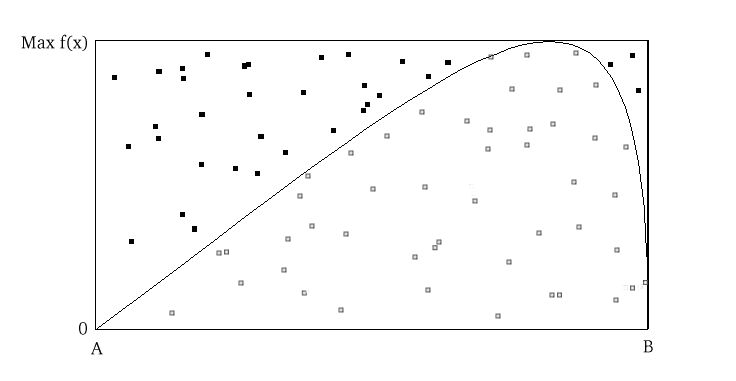
\includegraphics[scale=0.4]{reject.png}
    \end{center}
    \caption{Rejection sampling of a bounded form. Area is estimated by the ratio of accepted (open squares) to total points, multiplied by the rectangle area.}
    \label{fig:bound}
\end{figure}

Posit a function, $f(x)$ which can be evaluated for any value on the support of $x:S_x = [A,B]$, but may not be integrable or easily sampled from. If we can calculate the maximum  value of $f(x)$, we can then define a rectangle that is guaranteed to contain all possible values $(x,f(x))$. It is then trivial to generate points over the box and enumerate the values that fall under the curve (Figure \ref{fig:bound}).

\[
\frac{\mbox{Points under curve}}{\mbox{Points generated}} \times \mbox{box area} = \lim_{n \to \infty} \int_A^B f(x) dx
\]

\begin{figure}[h]
        \begin{center}
        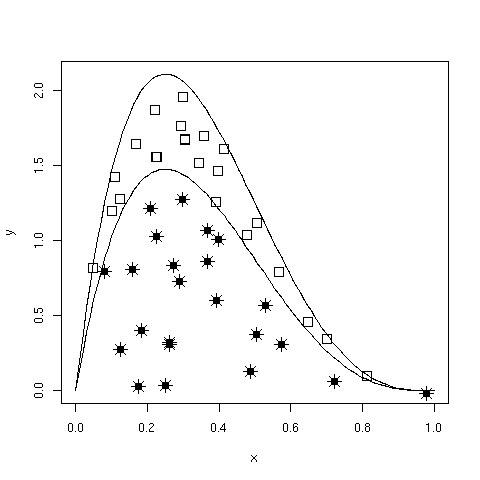
\includegraphics[scale=0.4]{envelope.png}
    \end{center}
    \caption{Rejection sampling of an unbounded form using an enveloping distribution.}
    \label{fig:unbound}
\end{figure}

\noindent This approach is useful, for example, in estimating the normalizing constant for posterior distributions.

If $f(x)$ has unbounded support (i.e. infinite tails), such as a Gaussian distribution, a bounding box is no longer appropriate. We must specify a majorizing (or, enveloping) function, $g(x)$, which implies:

\[
g(x) \ge  f(x) \qquad\forall x \in (-\infty,\infty)
\]

Having done this, we can now sample ${x_i}$ from $g(x)$ and accept or reject each of these values based upon $f(x_i)$. Specifically, for each draw $x_i$, we also draw a uniform random variate $u_i$ and accept $x_i$ if $u_i < f(x_i)/cg(x_i)$, where $c$ is a constant (Figure \ref{fig:unbound}). This approach is made more efficient by choosing an enveloping distribution that is ``close'' to the target distribution, thus maximizing the number of accepted points. Further improvement is gained by using optimized algorithms such as importance sampling which, as the name implies, samples more frequently from important areas of the distribution.

Rejection sampling is usually subject to declining performance as the dimension of the parameter space increases, so it is used less frequently than MCMC for evaluation of posterior distributions \citep{Gamerman:1997tb}.

%___________________________________________________________________________

\hypertarget{markov-chains}{}
\pdfbookmark[0]{Markov Chains}{markov-chains}
\section{Markov Chains}

A Markov chain is a special type of \emph{stochastic process}. The standard definition of a stochastic process is an ordered collection of random variables:

\[
\{X_t:t \in T\}
\]

\noindent where $t$ is frequently (but not necessarily) a time index. If we think of $X_t$ as a state $X$ at time $t$, and invoke the following dependence condition on each state:

\[
Pr(X_{t+1}=x_{t+1} | X_t=x_t, X_{t-1}=x_{t-1},\ldots,X_0=x_0) = Pr(X_{t+1}=x_{t+1} | X_t=x_t)
\]

\noindent then the stochastic process is known as a Markov chain. This conditioning specifies that the future depends on the current state, but not past states. Thus, the Markov chain wanders about the state space, remembering only where it has just been in the last time step. The collection of transition probabilities is sometimes called a \emph{transition matrix} when dealing with discrete states, or more generally, a \emph{transition kernel}. 

\noindent In the context of Markov chain Monte Carlo, it is useful to think of the Markovian property as ``mild non-independence''. MCMC allows us to indirectly generate independent samples from a particular posterior distribution.

%___________________________________________________________________________

\hypertarget{jargon-busting}{}
\pdfbookmark[1]{Jargon-busting}{jargon-busting}
\subsection{Jargon-busting}

Before we move on, it is important to define some general properties of Markov chains. They are frequently encountered in the MCMC literature, and some will help us decide whether MCMC is producing a useful sample from the posterior.

\begin{itemize}
\item \emph{Homogeneity}: A Markov chain is homogeneous at step $t$ if the transition probabilities are independent of time $t$.
\item \emph{Irreducibility}: A Markov chain is irreducible if every state is accessible in one or more steps from any other state. That is, the chain contains no absorbing states. This implies that there is a non-zero probability of eventually reaching state $k$ from any other state in the chain.
\item \emph{Recurrence}: States which are visited repeatedly are \emph{recurrent}. If the expected time to return to a particular state is bounded, this is known as \emph{positive recurrence}, otherwise the recurrent state is \emph{null recurrent}. Further, a chain is \emph{Harris recurrent} when it visits all states $X \in S$ infinitely often in the limit as $t \to \infty$; this is an important characteristic when dealing with unbounded, continuous state spaces. Whenever a chain ends up in a closed, irreducible set of Harris recurrent states, it stays there forever and visits every state with probability one.
\item \emph{Stationarity}: A stationary Markov chain produces the same marginal distribution when multiplied by the transition kernel.  Thus, if $P$ is some $n \times n$ transition matrix:

\[{\bf \pi P} = {\bf \pi}\]

\noindent for Markov chain $\pi$. Thus, $\pi$ is no longer subscripted, and is referred to as the \emph{limiting distribution} of the chain. In MCMC, the chain explores the state space according to its limiting marginal distribution.
\item \emph{Ergodicity}: Ergodicity is an emergent property of Markov chains which are irreducible, positive Harris recurrent and aperiodic. Ergodicity is defined as:

\[
\lim_{n \to \infty} Pr^{(n)}(\theta_i \rightarrow \theta_j) = \pi(\theta) \quad \forall \theta_i, \theta_j \in \Theta
\]

\noindent or in words, after many steps the marginal distribution of the chain is the same at one step as at all other steps. This implies that our Markov chain, which we recall is dependent, can generate samples that are independent if we wait long enough between samples. If it means anything to you, ergodicity is the analogue of the strong law of large numbers for Markov chains. For example, take values $\theta_{i+1},\ldots,\theta_{i+n}$ from a chain that has reached an ergodic state. A statistic of interest can then be estimated by:

\[
\frac{1}{n}\sum_{j=i+1}^{i+n} h(\theta_j) \approx \int f(\theta) h(\theta) d\theta
\]

\end{itemize}

%___________________________________________________________________________

\hypertarget{reversible-markov-chains}{}
\pdfbookmark[0]{Why MCMC Works: Reversible Markov Chains}{reversible-markov-chains}
\section{Why MCMC Works: Reversible Markov Chains}

Markov chain Monte Carlo simulates a Markov chain for which some function of interest (\emph{e.g.} the joint distribution of the parameters of some model) is the unique, invariant limiting distribution. An invariant distribution with respect to some Markov chain with transition kernel $Pr(y \mid x)$ implies that:
\[
\int_x Pr(y \mid x) \pi(x) dx = \pi(y).
\]

Invariance is guaranteed for any \textbf{reversible} Markov chain. Consider a Markov chain in reverse sequence: $\{\theta^{(n)},\theta^{(n-1)},...,\theta^{(0)}\}$. This sequence is still Markovian, because:
\[
Pr(\theta^{(k)}=y \mid \theta^{(k+1)}=x,\theta^{(k+2)}=x_1,\ldots ) = Pr(\theta^{(k)}=y \mid \theta^{(k+1)}=x)
\]
Forward and reverse transition probabilities may be related through Bayes theorem:
\begin{eqnarray}
Pr(\theta^{(k)}=y \mid \theta^{(k+1)}=x) &=& \frac{Pr(\theta^{(k+1)}=x \mid \theta^{(k)}=y) Pr(\theta^{(k)}=y)}{Pr(\theta^{(k+1)}=x)} \nonumber \\
&=& \frac{Pr(\theta^{(k+1)}=x \mid \theta^{(k)}=y) \pi^{(k)}(y)}{\pi^{(k+1)}(x)} \nonumber
\end{eqnarray}

\[
\frac{Pr(\theta^{(k+1)}=x \mid \theta^{(k)}=y) \pi^{(k)}(y)}{\pi^{(k+1)}(x)}
\]

\noindent Though not homogeneous in general, $\pi$ becomes homogeneous if \textbf{Do you ever call the stationary distribution itself homogeneous?}:
\begin{itemize}
\item $n \rightarrow \infty$
\item $\pi^{(0)}=\pi$ for some $i < k$ \textbf{Is it meant to be $\pi^(i)$, and }
\end{itemize}

\noindent If this chain is homogeneous it is called reversible, because it satisfies the \textbf{detailed balance equation}:
\[
\pi(x)Pr(y \mid x) = \pi(y) Pr(x \mid y)
\]
Reversibility is important because it has the effect of balancing movement through the entire state space. When a Markov chain is reversible, $\pi$ is the unique, invariant, stationary distribution of that chain.
Hence, if $\pi$ is of interest, we need only find the reversible Markov chain for which $\pi$ is the limiting distribution. This is what MCMC does!

%___________________________________________________________________________

\hypertarget{gibbs-sampling}{}
\pdfbookmark[0]{Gibbs Sampling}{gibbs-sampling}
\section{Gibbs Sampling}

The Gibbs sampler is the simplest and most prevalent MCMC algorithm. If a posterior has $k$ parameters to be estimated, we may condition each parameter on current values of the other $k-1$ parameters, and sample from the resultant distributional form (usually easier), and repeat this operation on the other parameters in turn. This procedure generates samples from the posterior distribution. Note that we have now combined Markov chains (conditional independence) and Monte Carlo techniques (estimation by simulation) to yield Markov chain Monte Carlo.

Here is a stereotypical Gibbs sampling algorithm:

\newcounter{lcount}
\begin{list}{\arabic{lcount}}
{\usecounter{lcount}}
\item Choose starting values for states (parameters): ${\bf \theta} = [\theta_1^{(0)},\theta_2^{(0)},\ldots,\theta_k^{(0)}]$
\item Initialize counter $j=1$
\item Draw the following values from each of the $k$ conditional distributions:
\begin{eqnarray*}
\theta_1^{(j)} &\sim& \pi(\theta_1 | \theta_2^{(j-1)},\theta_3^{(j-1)},\ldots,\theta_{k-1}^{(j-1)},\theta_k^{(j-1)}) \\
\theta_2^{(j)} &\sim& \pi(\theta_2 | \theta_1^{(j)},\theta_3^{(j-1)},\ldots,\theta_{k-1}^{(j-1)},\theta_k^{(j-1)}) \\
\theta_3^{(j)} &\sim& \pi(\theta_3 | \theta_1^{(j)},\theta_2^{(j)},\ldots,\theta_{k-1}^{(j-1)},\theta_k^{(j-1)}) \\
\vdots \\
\theta_{k-1}^{(j)} &\sim& \pi(\theta_{k-1} | \theta_1^{(j)},\theta_2^{(j)},\ldots,\theta_{k-2}^{(j)},\theta_k^{(j-1)}) \\
\theta_k^{(j)} &\sim& \pi(\theta_k | \theta_1^{(j)},\theta_2^{(j)},\theta_4^{(j)},\ldots,\theta_{k-2}^{(j)},\theta_{k-1}^{(j)})
\end{eqnarray*}
\item Increment $j$ and repeat until convergence occurs.
\end{list}

As we can see from the algorithm, each distribution is conditioned on the last iteration of its chain values, constituting a Markov chain as advertised. The Gibbs sampler has all of the important properties outlined in the previous section: it is aperiodic, homogeneous and ergodic. Once the sampler converges, all subsequent samples are from the target distribution. This convergence occurs at a geometric rate.

\hypertarget{the-metropolis-hastings-algorithm}{}
\pdfbookmark[0]{The Metropolis-Hastings Algorithm}{the-metropolis-hastings-algorithm}
\section{The Metropolis-Hastings Algorithm}

The key to success in applying the Gibbs sampler to the estimation of Bayesian posteriors is being able to specify the form of the complete conditionals of ${\bf \theta}$. In fact, the algorithm cannot be implemented without them. Of course, the posterior conditionals cannot always be neatly specified. In contrast to the Gibbs algorithm, the Metropolis-Hastings algorithm generates candidate state transitions from an alternate distribution, and accepts or rejects each candidate probabilistically.

Let us first consider a simple Metropolis-Hastings algorithm for a single parameter, $\theta$. We will use a standard sampling distribution, referred to as the \emph{proposal distribution}, to produce candidate variables $q_t(\theta^{\prime} | \theta)$. That is, the generated value, $\theta^{\prime}$, is a \emph{possible} next value for $\theta$ at step $t+1$. We also need to be able to calculate the probability of moving back to the original value from the candidate, or $q_t(\theta | \theta^{\prime})$. These probabilistic ingredients are used to define an \emph{acceptance ratio}:

\[
a(\theta^{\prime},\theta) = \frac{q_t(\theta^{\prime} | \theta) \pi(\theta^{\prime})}{q_t(\theta | \theta^{\prime}) \pi(\theta)}
\]

\noindent The value of $\theta^{(t+1)}$ is then determined by:

\[
\theta^{(t+1)} = \left\{\begin{array}{l@{\quad \mbox{with prob.} \quad}l}\theta^{\prime} & \min(a(\theta^{\prime},\theta),1) \\ \theta^{(t)} & 1 - \min(a(\theta^{\prime},\theta),1) \end{array}\right.
\]

\noindent This transition kernel implies that movement is not guaranteed at every step. It only occurs if the suggested transition is likely based on the acceptance ratio.

A single iteration of the Metropolis-Hastings algorithm proceeds as follows:

\newcounter{lcount2}
\begin{list}{\arabic{lcount2}}
{\usecounter{lcount2}}
\item Sample $\theta^{\prime}$ from $q(\theta^{\prime} | \theta^{(t)})$.
\item Generate a Uniform[0,1] random variate $u$.
\item If $a(\theta^{\prime},\theta) > u$ then $\theta^{(t+1)} = \theta^{\prime}$, otherwise $\theta^{(t+1)} = \theta^{(t)}$.
\end{list}

\noindent The original form of the algorithm specified by Metropolis required that $q_t(\theta^{\prime} | \theta) = q_t(\theta | \theta^{\prime})$, which reduces $a(\theta^{\prime},\theta)$ to $\pi(\theta^{\prime})/\pi(\theta)$, but this is not necessary. In either case, the state moves to high-density points in the distribution with high probability, and to low-density points with low probability. After convergence, the Metropolis-Hastings algorithm describes the full target posterior density, so all points are recurrent.

%___________________________________________________________________________

\hypertarget{random-walk-metropolis-hastings}{}
\pdfbookmark[1]{Random-walk Metropolis-Hastings}{random-walk-metropolis-hastings}
\subsection{Random-walk Metropolis-Hastings}

A practical implementation of the Metropolis-Hastings algorithm makes use of a random-walk proposal. Recall that a random walk is a Markov chain that evolves according to:

\begin{eqnarray*}
\theta^{(t+1)} &=& \theta^{(t)} + \epsilon_t \\
\epsilon_t &\sim& f(\phi)
\end{eqnarray*}

As applied to the MCMC sampling, the random walk is used as a proposal distribution, whereby dependent proposals are generated according to:

\[
q(\theta^{\prime} | \theta^{(t)}) = f(\theta^{\prime} - \theta^{(t)}) = \theta^{(t)} + \epsilon_t
\]

Generally, the density generating $\epsilon_t$ is symmetric about zero, resulting in a symmetric chain. Chain symmetry implies that $q(\theta^{\prime} | \theta^{(t)}) = q(\theta^{(t)} | \theta^{\prime})$, which reduces the Metropolis-Hastings acceptance ratio to:

\[
a(\theta^{\prime},\theta) = \frac{\pi(\theta^{\prime})}{\pi(\theta)}
\]

The choice of the random walk distribution for $\epsilon_t$ is frequently a normal or Student's $t$ density, but it may be any distribution that generates an irreducible proposal chain.

An important consideration is the specification of the scale parameter for the random walk error distribution. Large values produce random walk steps that are highly exploratory, but tend to produce proposal values in the tails of the target distribution, potentially resulting in very small acceptance rates. Conversely, small values tend to be accepted more frequently, since they tend to produce proposals close to the current parameter value, but may result in chains that mix very slowly. Some simulation studies suggest optimal acceptance rates in the range of 20-50\%. It is often worthwhile to optimize the proposal variance by iteratively adjusting its value, according to observed acceptance rates early in the MCMC simulation \citep{Gamerman:1997tb}.


\section[Distributions]{Probability distributions}
\label{sec:distributions}
% Generated by Sphinx.
%\usepackage[utf8]{inputenc}
%\usepackage[T1]{fontenc}
%\usepackage{babel}
%\usepackage{times}
%\usepackage[Bjarne]{fncychap}

\index{pymc.distributions (module)}

\newenvironment{paramlist}{
\begin{list}{}{
\setlength{\itemsep}{-2pt}
\setlength{\parsep}{-1pt}
\setlength{\topsep}{-1pt}}
 }{\end{list}}

 

\section{Discrete distributions}
\index{binomial\_like() (in module pymc.distributions)}

\hypertarget{pymc.distributions.binomial_like}{}\begin{funcdesc}{binomial\_like}{x, n, p}
Binomial log-likelihood.  The discrete probability distribution of the
number of successes in a sequence of n independent yes/no experiments,
each of which yields success with probability p.
\begin{gather}
\begin{split}f(x \mid n, p) = \frac{n!}{x!(n-x)!} p^x (1-p)^{1-x}\end{split}\notag\\\begin{split}\end{split}\notag
\end{gather}
\paragraph{Parameters}
\begin{paramlist}
\item[] \textbf{x} : float
\begin{quote}

Number of successes, \textgreater{} 0.
\end{quote}

\item[]  \textbf{n} : int
\begin{quote}

Number of Bernoulli trials, \textgreater{} x.
\end{quote}

\item[] \textbf{p} : float
\begin{quote}

Probability of success in each trial, $p \in [0,1]$.
\end{quote}
\end{paramlist}
\paragraph{Notes}
\begin{itemize}
\item {} 
$E(X)=np$

\item {} 
$Var(X)=np(1-p)$

\end{itemize}
\end{funcdesc}


\index{geometric\_like() (in module pymc.distributions)}
\hypertarget{pymc.distributions.geometric_like}{}\begin{funcdesc}{geometric\_like}{x, p}
Geometric log-likelihood. The probability that the first success in a
sequence of Bernoulli trials occurs after x trials.
\begin{gather}
\begin{split}f(x \mid p) = p(1-p)^{x-1}\end{split}\notag\\\begin{split}\end{split}\notag
\end{gather}
\paragraph{Parameters}
\begin{paramlist}
\item[] \textbf{x} : int
\begin{quote}

Number of trials before first success, \textgreater{} 0.
\end{quote}

\item[] \textbf{p} : float
\begin{quote}

Probability of success on an individual trial, $p \in [0,1]$
\end{quote}
\end{paramlist}
\paragraph{Notes}
\begin{itemize}
\item {} 
$E(X)=1/p$

\item {} 
$Var(X)=\frac{1-p}{p^2}$

\end{itemize}
\end{funcdesc}
\index{poisson\_like() (in module pymc.distributions)}

\hypertarget{pymc.distributions.poisson_like}{}\begin{funcdesc}{poisson\_like}{x, mu}
Poisson log-likelihood. The Poisson is a discrete probability distribution.
It expresses the probability of a number of events occurring in a fixed
period of time if these events occur with a known average rate, and are
independent of the time since the last event. The Poisson distribution can
be derived as a limiting case of the binomial distribution.
\begin{gather}
\begin{split}f(x \mid \mu) = \frac{e^{-\mu}\mu^x}{x!}\end{split}\notag\\\begin{split}\end{split}\notag
\end{gather}
\paragraph{Parameters}
\begin{paramlist}
\item[]\textbf{x} : int
\begin{quote}

$x \in {0,1,2,...}$
\end{quote}

\item[]\textbf{mu} : float
\begin{quote}

Expected number of occurrences that occur during the given interval,
$\mu \geq 0$.
\end{quote}
\end{paramlist}
\paragraph{Notes}
\begin{itemize}
\item {} 
$E(x)=\mu$

\item {} 
$Var(x)=\mu$

\end{itemize}
\end{funcdesc}
\index{negative\_binomial\_like() (in module pymc.distributions)}

\hypertarget{pymc.distributions.negative_binomial_like}{}\begin{funcdesc}{negative\_binomial\_like}{x, mu, alpha}
Negative binomial log-likelihood
\begin{gather}
\begin{split}f(x \mid \mu, \alpha) = \frac{\Gamma(x+\alpha)}{x! \Gamma(\alpha)} (\alpha/(\mu+\alpha))^\alpha (\mu/(\mu+\alpha))^x\end{split}\notag\\\begin{split}\end{split}\notag
\end{gather}
x \textgreater{} 0, mu \textgreater{} 0, alpha \textgreater{} 0
\paragraph{Notes}
In Wikipedia's parameterization, $r=\alpha$, $p=\alpha/(\mu+\alpha)$ and $\mu=r(1-p)/p$.
This parameterization is convenient in the Gamma-Poisson mixture interpretation
of the negative binomial distribution. In that case the expectation of the rate
is equal to $\mu$.
\end{funcdesc}

\index{categorical\_like() (in module pymc.distributions)}
\hypertarget{pymc.distributions.categorical_like}{}\begin{funcdesc}{categorical\_like}{x, p}
Categorical log-likelihood.
\begin{gather}
\begin{split}f(x=v_i \mid p) = p_i\end{split}\notag\\\begin{split}\end{split}\notag
\end{gather}\begin{gather}
\begin{split}v_i \in 0 \ldots k-1\end{split}\notag\\\begin{split}\end{split}\notag
\end{gather}
\paragraph{Parameters}
\begin{paramlist}
\item[] \textbf{x} : integer
\begin{quote}

$x \in v$
$v_i \in 0 \ldots k-1$
\end{quote}

\item[]\textbf{p} : (k) float
\begin{quote}

$p > 0$
$\sum p = 1$
\end{quote}
\end{paramlist}
\end{funcdesc}
\index{discrete\_uniform\_like() (in module pymc.distributions)}

\hypertarget{pymc.distributions.discrete_uniform_like}{}\begin{funcdesc}{discrete\_uniform\_like}{x, lower, upper}
discrete\_uniform log-likelihood.
\begin{gather}
\begin{split}f(x \mid lower, upper) = \frac{1}{upper-lower}\end{split}\notag\\\begin{split}\end{split}\notag
\end{gather}
\paragraph{Parameters}
\begin{paramlist}
\item[] \textbf{x} : float
\begin{quote}

$lower \geq x \geq upper$
\end{quote}

\item[] \textbf{lower} : float
\begin{quote}

Lower limit.
\end{quote}

\item[] \textbf{upper} : float
\begin{quote}

Upper limit.
\end{quote}
\end{paramlist}
\end{funcdesc}


\section{Continuous distributions}
\index{bernoulli\_like() (in module pymc.distributions)}

\hypertarget{pymc.distributions.bernoulli_like}{}\begin{funcdesc}{bernoulli\_like}{x, p}
Bernoulli log-likelihood

The Bernoulli distribution describes the probability of successes (x=1) and
failures (x=0).
\begin{gather}
\begin{split}f(x \mid p) = p^{x- 1} (1-p)^{1-x}\end{split}\notag\\\begin{split}\end{split}\notag
\end{gather}
\paragraph{Parameters}
\begin{paramlist}
\item[] \textbf{x} : sequence
\begin{quote}

Series of successes (1) and failures (0). $x=0,1$
\end{quote}

\item[] \textbf{p} : float
\begin{quote}

Probability of success. $0 < p < 1$.
\end{quote}
\end{paramlist}
\paragraph{Notes}
\begin{itemize}
\item {} 
$E(x)= p$

\item {} 
$Var(x)= p(1-p)$

\end{itemize}

\end{funcdesc}
\index{beta\_like() (in module pymc.distributions)}

\hypertarget{pymc.distributions.beta_like}{}\begin{funcdesc}{beta\_like}{x, alpha, beta}
Beta log-likelihood.
\begin{gather}
\begin{split}f(x \mid \alpha, \beta) = \frac{\Gamma(\alpha + \beta)}{\Gamma(\alpha) \Gamma(\beta)} x^{\alpha - 1} (1 - x)^{\beta - 1}\end{split}\notag\\\begin{split}\end{split}\notag
\end{gather}
\paragraph{Parameters}
\begin{paramlist}
\item[] \textbf{x} : float
\begin{quote}

0 \textless{} x \textless{} 1
\end{quote}

\item[] \textbf{alpha} : float
\begin{quote}

\textgreater{} 0
\end{quote}

\item[] \textbf{beta} : float
\begin{quote}

\textgreater{} 0
\end{quote}
\end{paramlist}
\paragraph{Notes}
\begin{itemize}
\item {} 
$E(X)=\frac{\alpha}{\alpha+\beta}$

\item {} 
$Var(X)=\frac{\alpha \beta}{(\alpha+\beta)^2(\alpha+\beta+1)}$

\end{itemize}

\end{funcdesc}
\index{cauchy\_like() (in module pymc.distributions)}

\hypertarget{pymc.distributions.cauchy_like}{}\begin{funcdesc}{cauchy\_like}{x, alpha, beta}
Cauchy log-likelihood. The Cauchy distribution is also known as the
Lorentz or the Breit-Wigner distribution.
\begin{gather}
\begin{split}f(x \mid \alpha, \beta) = \frac{1}{\pi \beta [1 + (\frac{x-\alpha}{\beta})^2]}\end{split}\notag\\\begin{split}\end{split}\notag
\end{gather}
\paragraph{Parameters}
\begin{paramlist}
\item[] \textbf{alpha} : float
\begin{quote}

Location parameter.
\end{quote}

\item[] \textbf{beta} : float
\begin{quote}

Scale parameter \textgreater{} 0.
\end{quote}
\end{paramlist}
\paragraph{Notes}
\begin{itemize}
\item {} 
Mode and median are at alpha.

\end{itemize}
\end{funcdesc}
\index{chi2\_like() (in module pymc.distributions)}

\hypertarget{pymc.distributions.chi2_like}{}\begin{funcdesc}{chi2\_like}{x, nu}
Chi-squared $\chi^2$ log-likelihood.
\begin{gather}
\begin{split}f(x \mid \nu) = \frac{x^{(\nu-2)/2}e^{-x/2}}{2^{\nu/2}\Gamma(\nu/2)}\end{split}\notag\\\begin{split}\end{split}\notag
\end{gather}
\paragraph{Parameters}
\begin{paramlist}
\item[] \textbf{x} : float
\begin{quote}

$\ge 0$
\end{quote}

\item[] \textbf{nu} : int
\begin{quote}

Degrees of freedom ( $nu > 0$)
\end{quote}
\end{paramlist}
\paragraph{Notes}
\begin{itemize}
\item {} 
$E(X)=\nu$

\item {} 
$Var(X)=2\nu$

\end{itemize}
\end{funcdesc}
\index{degenerate\_like() (in module pymc.distributions)}

\hypertarget{pymc.distributions.degenerate_like}{}\begin{funcdesc}{degenerate\_like}{x, k}
Degenerate log-likelihood.
\begin{gather}
\begin{split}f(x \mid k) = \left\{ \begin{matrix} 1 \text{ if } x = k \\ 0 \text{ if } x \ne k\end{matrix} \right.\end{split}\notag\\\begin{split}\end{split}\notag
\end{gather}
\paragraph{Parameters}
\begin{paramlist}
\item[] \textbf{x} : float
\begin{quote}

$x = k$
\end{quote}

\item[] \textbf{k} : float
\begin{quote}

degenerate value.
\end{quote}
\end{paramlist}
\end{funcdesc}
\index{exponential\_like() (in module pymc.distributions)}

\hypertarget{pymc.distributions.exponential_like}{}\begin{funcdesc}{exponential\_like}{x, beta}
Exponential log-likelihood.

The exponential distribution is a special case of the gamma distribution
with alpha=1. It often describes the duration of an event.
\begin{gather}
\begin{split}f(x \mid \beta) = \frac{1}{\beta}e^{-x/\beta}\end{split}\notag\\\begin{split}\end{split}\notag
\end{gather}
\paragraph{Parameters}
\begin{paramlist}
\item[] \textbf{x} : float
\begin{quote}

$x \ge 0$
\end{quote}

\item[] \textbf{beta} : float
\begin{quote}

Survival parameter $\beta > 0$
\end{quote}
\end{paramlist}
\paragraph{Notes}
\begin{itemize}
\item {} 
$E(X) = \beta$

\item {} 
$Var(X) = \beta^2$

\end{itemize}
\end{funcdesc}
\index{exponweib\_like() (in module pymc.distributions)}

\hypertarget{pymc.distributions.exponweib_like}{}\begin{funcdesc}{exponweib\_like}{x, alpha, k, loc=0, scale=1}
Exponentiated Weibull log-likelihood.

The exponentiated Weibull distribution is a generalization of the Weibull
family. Its value lies in being able to model monotone and non-monotone
failure rates.
\begin{gather}
\begin{split}f(x \mid \alpha,k,loc,scale)  & = \frac{\alpha k}{scale} (1-e^{-z^k})^{\alpha-1} e^{-z^k} z^{k-1} \\
z & = \frac{x-loc}{scale}\end{split}\notag\\\begin{split}\end{split}\notag
\end{gather}\paragraph{Parameters}
\begin{paramlist}
\item[] \textbf{x} : float
\begin{quote}

\textgreater{} 0
\end{quote}

\item[] \textbf{alpha} : float
\begin{quote}

Shape parameter
\end{quote}

\item[] \textbf{k} : float
\begin{quote}

\textgreater{} 0
\end{quote}

\item[] \textbf{loc} : float
\begin{quote}

Location parameter
\end{quote}

\item[] \textbf{scale} : float
\begin{quote}

Scale parameter \textgreater{} 0.
\end{quote}
\end{paramlist}
\end{funcdesc}
\index{gamma\_like() (in module pymc.distributions)}

\hypertarget{pymc.distributions.gamma_like}{}\begin{funcdesc}{gamma\_like}{x, alpha, beta}
Gamma log-likelihood.

Represents the sum of alpha exponentially distributed random variables, each
of which has mean beta.
\begin{gather}
\begin{split}f(x \mid \alpha, \beta) = \frac{\beta^{\alpha}x^{\alpha-1}e^{-\beta x}}{\Gamma(\alpha)}\end{split}\notag\\\begin{split}\end{split}\notag
\end{gather}
\paragraph{Parameters}
\begin{paramlist}
\item[] \textbf{x} : float
\begin{quote}

$x \ge 0$
\end{quote}

\item[] \textbf{alpha} : float
\begin{quote}

Shape parameter $\alpha > 0$.
\end{quote}

\item[] \textbf{beta} : float
\begin{quote}

Scale parameter $\beta > 0$.
\end{quote}
\end{paramlist}
\paragraph{Notes}
\begin{itemize}
\item {} 
$E(X) = \frac{\alpha}{\beta}$

\item {} 
$Var(X) = \frac{\alpha}{\beta^2}$

\end{itemize}
\end{funcdesc}
\index{half\_normal\_like() (in module pymc.distributions)}

\hypertarget{pymc.distributions.half_normal_like}{}\begin{funcdesc}{half\_normal\_like}{x, tau}
Half-normal log-likelihood, a normal distribution with mean 0 and limited
to the domain $x \in [0, \infty)$.
\begin{gather}
\begin{split}f(x \mid \tau) = \sqrt{\frac{2\tau}{\pi}}\exp\left\{ {\frac{-x^2 \tau}{2}}\right\}\end{split}\notag\\\begin{split}\end{split}\notag
\end{gather}
\paragraph{Parameters}
\begin{paramlist}
\item[] \textbf{x} : float
\begin{quote}

$x \ge 0$
\end{quote}

\item[] \textbf{tau} : float
\begin{quote}

$\tau > 0$
\end{quote}
\end{paramlist}
\end{funcdesc}
\index{hypergeometric\_like() (in module pymc.distributions)}

\hypertarget{pymc.distributions.hypergeometric_like}{}\begin{funcdesc}{hypergeometric\_like}{x, n, m, N}
Hypergeometric log-likelihood. Discrete probability distribution that
describes the number of successes in a sequence of draws from a finite
population without replacement.
\begin{gather}
\begin{split}f(x \mid n, m, N) = \frac{\binom{m}{x}\binom{N-m}{n-x}}{\binom{N}{n}}\end{split}\notag\\\begin{split}\end{split}\notag
\end{gather}
\paragraph{Parameters}
\begin{paramlist}
\item[] \textbf{x} : int
\begin{quote}
Number of successes in a sample drawn from a population.
$\max(0, draws-failures) \leq x \leq \min(draws, success)$
\end{quote}
\item[] \textbf{n} : int
\begin{quote}
Size of sample drawn from the population.
\end{quote}
\item[] \textbf{m} : int
\begin{quote}
Number of successes in the population.
\end{quote}
\item[] \textbf{N} : int
\begin{quote}
Total number of units in the population.
\end{quote}
\end{paramlist}
\paragraph{Notes}
\begin{itemize}
\item $E(X) = \frac{n n}{N}$
\end{itemize}
\end{funcdesc}
\index{inverse\_gamma\_like() (in module pymc.distributions)}

\hypertarget{pymc.distributions.inverse_gamma_like}{}\begin{funcdesc}{inverse\_gamma\_like}{x, alpha, beta}
Inverse gamma log-likelihood, the reciprocal of the gamma distribution.
\begin{gather}
\begin{split}f(x \mid \alpha, \beta) = \frac{\beta^{\alpha}}{\Gamma(\alpha)} x^{-\alpha - 1} \exp\left(\frac{-\beta}{x}\right)\end{split}\notag\\\begin{split}\end{split}\notag
\end{gather}
\paragraph{Parameters}
\begin{paramlist}
\item[] \textbf{x} : float
\begin{quote}

x \textgreater{} 0
\end{quote}

\item[] \textbf{alpha} : float
\begin{quote}

Shape parameter, $\alpha > 0$.
\end{quote}

\item[] \textbf{beta} : float
\begin{quote}

Scale parameter, $\beta > 0$.
\end{quote}
\end{paramlist}
\paragraph{Notes}
\begin{itemize}
\item $E(X)=\frac{1}{\beta(\alpha-1)}$  for $\alpha > 1$.
\end{itemize}
\end{funcdesc}
\index{laplace\_like() (in module pymc.distributions)}

\hypertarget{pymc.distributions.laplace_like}{}\begin{funcdesc}{laplace\_like}{x, mu, tau}
Laplace (doubel exponential) log-likelihood.

The Laplace (or double eexponential) distribution describes the
difference between two independent, identically distributed exponential
events. It is often used as a heavier-tailed alternative to the normal.
\begin{gather}
\begin{split}f(x \mid \mu, \tau) = \frac{\tau}{2}e^{-\tau|x-\mu|}\end{split}\notag\\\begin{split}\end{split}\notag
\end{gather}\paragraph{Parameters}\begin{paramlist}

\item[] \textbf{x} : float
\begin{quote}

$-\infty < x < \infty$
\end{quote}

\item[] \textbf{mu} : float
\begin{quote}

Location parameter $-\infty < \mu < \infty$
\end{quote}

\item[] \textbf{tau} : float
\begin{quote}

Scale parameter $\tau > 0$
\end{quote}
\end{paramlist}
\paragraph{Notes}
\begin{itemize}
\item {} 
$E(X) = \mu$

\item {} 
$Var(X) = \frac{2}{\tau^2}$

\end{itemize}
\end{funcdesc}
\index{logistic\_like() (in module pymc.distributions)}

\hypertarget{pymc.distributions.logistic_like}{}\begin{funcdesc}{logistic\_like}{x, mu, tau}
Logistic log-likelihood.

The logistic distribution is often used as a growth model; for example,
populations, markets. Resembles a heavy-tailed normal distribution.
\begin{gather}
\begin{split}f(x \mid \mu, \tau) = \frac{\tau \exp(-\tau[x-\mu])}{[1 + \exp(-\tau[x-\mu])]^2}\end{split}\notag\\\begin{split}\end{split}\notag
\end{gather}\paragraph{Parameters}\begin{paramlist}

\item[] \textbf{x} : float
\begin{quote}

$-\infty < x < \infty$
\end{quote}

\item[] \textbf{mu} : float
\begin{quote}

Location parameter $-\infty < \mu < \infty$
\end{quote}

\item[] \textbf{tau} : float
\begin{quote}

Scale parameter $\tau > 0$
\end{quote}
\end{paramlist}
\paragraph{Notes}
\begin{itemize}
\item {} 
$E(X) = \mu$

\item {} 
$Var(X) = \frac{\pi^2}{3\tau^2}$

\end{itemize}
\end{funcdesc}
\index{lognormal\_like() (in module pymc.distributions)}

\hypertarget{pymc.distributions.lognormal_like}{}\begin{funcdesc}{lognormal\_like}{x, mu, tau}
Log-normal log-likelihood. Distribution of any random variable whose
logarithm is normally distributed. A variable might be modeled as
log-normal if it can be thought of as the multiplicative product of many
small independent factors.
\begin{gather}
\begin{split}f(x \mid \mu, \tau) = \sqrt{\frac{\tau}{2\pi}}\frac{
\exp\left\{ -\frac{\tau}{2} (\ln(x)-\mu)^2 \right\}}{x}\end{split}\notag\\\begin{split}\end{split}\notag
\end{gather}\paragraph{Parameters}\begin{paramlist}

\item[] \textbf{x} : float
\begin{quote}

x \textgreater{} 0
\end{quote}

\item[] \textbf{mu} : float
\begin{quote}

Location parameter.
\end{quote}

\item[] \textbf{tau} : float
\begin{quote}

Scale parameter, \textgreater{} 0.
\end{quote}
\end{paramlist}
\paragraph{Notes}

$E(X)=e^{\mu+\frac{1}{2\tau}}$
\end{funcdesc}
\index{normal\_like() (in module pymc.distributions)}

\hypertarget{pymc.distributions.normal_like}{}\begin{funcdesc}{normal\_like}{x, mu, tau}
Normal log-likelihood.
\begin{gather}
\begin{split}f(x \mid \mu, \tau) = \sqrt{\frac{\tau}{2\pi}} \exp\left\{ -\frac{\tau}{2} (x-\mu)^2 \right\}\end{split}\notag\\\begin{split}\end{split}\notag
\end{gather}\paragraph{Parameters}\begin{paramlist}

\item[] \textbf{x} : float
\begin{quote}

Input data.
\end{quote}

\item[] \textbf{mu} : float
\begin{quote}

Mean of the distribution.
\end{quote}

\item[] \textbf{tau} : float
\begin{quote}

Precision of the distribution, \textgreater{} 0 ( corresponds to 1/sigma**2 ).
\end{quote}
\end{paramlist}
\paragraph{Notes}
\begin{itemize}
\item {} 
$E(X) = \mu$

\item {} 
$Var(X) = 1/\tau$

\end{itemize}
\end{funcdesc}
\index{t\_like() (in module pymc.distributions)}

\hypertarget{pymc.distributions.t_like}{}\begin{funcdesc}{t\_like}{x, nu}
Student's t log-likelihood
\begin{gather}
\begin{split}f(x \mid \nu) = \frac{\Gamma(\frac{\nu+1}{2})}{\Gamma(\frac{\nu}{2}) \sqrt{\nu\pi}} \left( 1 + \frac{x^2}{\nu} \right)^{-\frac{\nu+1}{2}}\end{split}\notag\\\begin{split}\end{split}\notag
\end{gather}\paragraph{Parameters}\begin{paramlist}

\item[] \textbf{x} : float
\begin{quote}

Input data.
\end{quote}

\item[] \textbf{nu} : float
\begin{quote}

Degrees of freedom.
\end{quote}
\end{paramlist}
\end{funcdesc}
\index{uniform\_like() (in module pymc.distributions)}

\hypertarget{pymc.distributions.uniform_like}{}\begin{funcdesc}{uniform\_like}{x, lower, upper}
Uniform log-likelihood.
\begin{gather}
\begin{split}f(x \mid lower, upper) = \frac{1}{upper-lower}\end{split}\notag\\\begin{split}\end{split}\notag
\end{gather}\paragraph{Parameters}\begin{paramlist}

\item[] \textbf{x} : float
\begin{quote}

$lower \geq x \geq upper$
\end{quote}

\item[] \textbf{lower} : float
\begin{quote}

Lower limit.
\end{quote}

\item[] \textbf{upper} : float
\begin{quote}

Upper limit.
\end{quote}
\end{paramlist}
\end{funcdesc}
\index{weibull\_like() (in module pymc.distributions)}

\hypertarget{pymc.distributions.weibull_like}{}\begin{funcdesc}{weibull\_like}{x, alpha, beta}
Weibull log-likelihood
\begin{gather}
\begin{split}f(x \mid \alpha, \beta) = \frac{\alpha x^{\alpha - 1}
\exp(-(\frac{x}{\beta})^{\alpha})}{\beta^\alpha}\end{split}\notag\\\begin{split}\end{split}\notag
\end{gather}\paragraph{Parameters}\begin{paramlist}

\item[] \textbf{x} : float
\begin{quote}

$x \ge 0$
\end{quote}

\item[] \textbf{alpha} : float
\begin{quote}

\textgreater{} 0
\end{quote}

\item[] \textbf{beta} : float
\begin{quote}

\textgreater{} 0
\end{quote}
\end{paramlist}
\paragraph{Notes}
\begin{itemize}
\item {} 
$E(x)=\beta \Gamma(1+\frac{1}{\alpha})$

\item {} 
$Var(x)=\beta^2 \Gamma(1+\frac{2}{\alpha} - \mu^2)$

\end{itemize}
\end{funcdesc}
\index{skew\_normal\_like() (in module pymc.distributions)}

\hypertarget{pymc.distributions.skew_normal_like}{}\begin{funcdesc}{skew\_normal\_like}{x, mu, tau, alpha}
Azzalini's skew-normal log-likelihood
\begin{gather}
\begin{split}f(x \mid \mu, \tau, \alpha) = 2 \Phi((x-\mu)\sqrt{\tau}\alpha) \phi(x,\mu,\tau)\end{split}\notag\\\begin{split}\end{split}\notag
\end{gather}\paragraph{Parameters}\begin{paramlist}

\item[] \textbf{x} : float
\begin{quote}

Input data.
\end{quote}

\item[] \textbf{mu} : float
\begin{quote}

Mean of the distribution.
\end{quote}

\item[] \textbf{tau} : float
\begin{quote}

Precision of the distribution, \textgreater{} 0.
\end{quote}

\item[] \textbf{alpha} : float
\begin{quote}

Shape parameter of the distribution.
\end{quote}
\end{paramlist}
\paragraph{Notes}
\begin{itemize}
\item {} 
See \href{http://azzalini.stat.unipd.it/SN/}{http://azzalini.stat.unipd.it/SN/}

\end{itemize}
\end{funcdesc}
\index{truncnorm\_like() (in module pymc.distributions)}

\hypertarget{pymc.distributions.truncnorm_like}{}\begin{funcdesc}{truncnorm\_like}{x, mu, tau, a, b}
Truncated normal log-likelihood.
\begin{gather}
\begin{split}f(x \mid \mu, \tau, a, b) = \frac{\phi(\frac{x-\mu}{\sigma})} {\Phi(\frac{b-\mu}{\sigma}) - \Phi(\frac{a-\mu}{\sigma})},\end{split}\notag\\\begin{split}\end{split}\notag
\end{gather}
where $\sigma^2=1/\tau$.
\paragraph{Parameters}\begin{paramlist}

\item[] \textbf{x} : float
\begin{quote}

Input data.
\end{quote}

\item[] \textbf{mu} : float
\begin{quote}

Mean of the distribution.
\end{quote}

\item[] \textbf{tau} : float
\begin{quote}

Precision of the distribution, \textgreater{} 0 ( corresponds to 1/sigma**2 ).
\end{quote}

\item[] \textbf{a} : float
\begin{quote}

Left bound of the distribution.
\end{quote}

\item[] \textbf{b} : float
\begin{quote}

Right bound of the distribution.
\end{quote}
\end{paramlist}
\end{funcdesc}


\section{Multivariate discrete distributions}
\index{multivariate\_hypergeometric\_like() (in module pymc.distributions)}

\hypertarget{pymc.distributions.multivariate_hypergeometric_like}{}\begin{funcdesc}{multivariate\_hypergeometric\_like}{x, m}
The multivariate hypergeometric describes the probability of drawing x{[}i{]}
elements of the ith category, when the number of items in each category is
given by m.
\begin{gather}
\begin{split}\frac{\prod_i \binom{m_i}{x_i}}{\binom{N}{n}}\end{split}\notag\\\begin{split}\end{split}\notag
\end{gather}
where $N = \sum_i m_i$ and $n = \sum_i x_i$.
\paragraph{Parameters}\begin{paramlist}

\item[] \textbf{x} : int sequence
\begin{quote}

Number of draws from each category, $< m$
\end{quote}

\item[] \textbf{m} : int sequence
\begin{quote}

Number of items in each categoy.
\end{quote}
\end{paramlist}
\end{funcdesc}
\index{multinomial\_like() (in module pymc.distributions)}

\hypertarget{pymc.distributions.multinomial_like}{}\begin{funcdesc}{multinomial\_like}{x, n, p}
Multinomial log-likelihood. Generalization of the binomial
distribution, but instead of each trial resulting in ``success'' or
``failure'', each one results in exactly one of some fixed finite number k
of possible outcomes over n independent trials. `x{[}i{]}' indicates the number
of times outcome number i was observed over the n trials.
\begin{gather}
\begin{split}f(x \mid n, p) = \frac{n!}{\prod_{i=1}^k x_i!} \prod_{i=1}^k p_i^{x_i}\end{split}\notag\\\begin{split}\end{split}\notag
\end{gather}\paragraph{Parameters}\begin{paramlist}

\item[] \textbf{x} : (ns, k) int
\begin{quote}

Random variable indicating the number of time outcome i is observed,
$\sum_{i=1}^k x_i=n$, $x_i \ge 0$.
\end{quote}

\item[] \textbf{n} : int
\begin{quote}

Number of trials.
\end{quote}

\item[] \textbf{p} : (k,) float
\begin{quote}

Probability of each one of the different outcomes,
$\sum_{i=1}^k p_i = 1)$, $p_i \ge 0$.
\end{quote}
\end{paramlist}
\paragraph{Notes}
\begin{itemize}
\item {} 
$E(X_i)=n p_i$

\item {} 
$var(X_i)=n p_i(1-p_i)$

\item {} 
$cov(X_i,X_j) = -n p_i p_j$

\end{itemize}
\end{funcdesc}


\section{Multivariate continuous distributions}
\index{dirichlet\_like() (in module pymc.distributions)}

\hypertarget{pymc.distributions.dirichlet_like}{}\begin{funcdesc}{dirichlet\_like}{x, theta}
Dirichlet log-likelihood.

This is a multivariate continuous distribution.
\begin{gather}
\begin{split}f(\mathbf{x}) = \frac{\Gamma(\sum_{i=1}^k \theta_i)}{\prod \Gamma(\theta_i)} \prod_{i=1}^k x_i^{\theta_i - 1}\end{split}\notag\\\begin{split}\end{split}\notag
\end{gather}\paragraph{Parameters}\begin{paramlist}

\item[] \textbf{x} : (n,k-1) array
\begin{quote}

Where \emph{n} is the number of samples and \emph{k} the dimension.
$0 < x_i < 1$,  $\sum_{i=1}^{k-1} x_i < 1$
\end{quote}

\item[] \textbf{theta} : (n,k) or (1,k) float
\begin{quote}

$\theta > 0$
\end{quote}
\end{paramlist}
\end{funcdesc}
\index{inverse\_wishart\_like() (in module pymc.distributions)}

\hypertarget{pymc.distributions.inverse_wishart_like}{}\begin{funcdesc}{inverse\_wishart\_like}{X, n, Tau}
Inverse Wishart log-likelihood. The inverse Wishart distribution is the conjugate 
prior for the covariance matrix of a multivariate normal distribution.
\begin{gather}
\begin{split}f(X \mid n, T) = \frac{{\mid T \mid}^{n/2}{\mid X \mid}^{(n-k-1)/2} \exp\left\{ -\frac{1}{2} Tr(TX^{-1}) \right\}}{2^{nk/2} \Gamma_p(n/2)}\end{split}\notag\\\begin{split}\end{split}\notag
\end{gather}
where $k$ is the rank of X.
\paragraph{Parameters}\begin{paramlist}

\item[] \textbf{X} : matrix
\begin{quote}

Symmetric, positive definite.
\end{quote}

\item[] \textbf{n} : int
\begin{quote}

Degrees of freedom, \textgreater{} 0.
\end{quote}

\item[] \textbf{Tau} : matrix
\begin{quote}

Symmetric and positive definite
\end{quote}
\end{paramlist}
\end{funcdesc}
\index{mv\_normal\_like() (in module pymc.distributions)}

\hypertarget{pymc.distributions.mv_normal_like}{}\begin{funcdesc}{mv\_normal\_like}{x, mu, tau}
Multivariate normal log-likelihood
\begin{gather}
\begin{split}f(x \mid \pi, T) = \frac{T^{n/2}}{(2\pi)^{1/2}} \exp\left\{ -\frac{1}{2} (x-\mu)^{\prime}T(x-\mu) \right\}\end{split}\notag\\\begin{split}\end{split}\notag
\end{gather}\paragraph{Parameters}\begin{paramlist}

\item[] \textbf{x: (n,k)} :

\item[] \textbf{mu: (k)} :

\item[] \textbf{tau: (k,k)} :

\item[] \textbf{tau positive definite} :
\end{paramlist}

\strong{See Also:}


\hyperlink{pymc.distributions.mv_normal_chol_like}{\code{mv\_normal\_chol\_like}}, \hyperlink{pymc.distributions.mv_normal_cov_like}{\code{mv\_normal\_cov\_like}}


\end{funcdesc}
\index{mv\_normal\_cov\_like() (in module pymc.distributions)}

\hypertarget{pymc.distributions.mv_normal_cov_like}{}\begin{funcdesc}{mv\_normal\_cov\_like}{x, mu, C}
Multivariate normal log-likelihood
\begin{gather}
\begin{split}f(x \mid \pi, C) = \frac{T^{n/2}}{(2\pi)^{1/2}} \exp\left\{ -\frac{1}{2} (x-\mu)^{\prime}C^{-1}(x-\mu) \right\}\end{split}\notag\\\begin{split}\end{split}\notag
\end{gather}
x: (n,k)
mu: (k)
C: (k,k)
C positive definite


\strong{See Also:}


\hyperlink{pymc.distributions.mv_normal_like}{\code{mv\_normal\_like}}, \hyperlink{pymc.distributions.mv_normal_chol_like}{\code{mv\_normal\_chol\_like}}


\end{funcdesc}
\index{mv\_normal\_chol\_like() (in module pymc.distributions)}

\hypertarget{pymc.distributions.mv_normal_chol_like}{}\begin{funcdesc}{mv\_normal\_chol\_like}{x, mu, tau}
Multivariate normal log-likelihood
\begin{gather}
\begin{split}f(x \mid \pi, \sigma) = \frac{T^{n/2}}{(2\pi)^{1/2}} \exp\left\{ -\frac{1}{2} (x-\mu)^{\prime}\sigma \sigma^{\prime}(x-\mu) \right\}\end{split}\notag\\\begin{split}\end{split}\notag
\end{gather}\paragraph{Parameters}\begin{paramlist}

\item[] \textbf{x} : (n,k)

\item[] \textbf{mu} : (k)

\item[] \textbf{sigma} : (k,k)

\item[] \textbf{sigma lower triangular} :
\end{paramlist}

\strong{See Also:}


\hyperlink{pymc.distributions.mv_normal_like}{\code{mv\_normal\_like}}, \hyperlink{pymc.distributions.mv_normal_cov_like}{\code{mv\_normal\_cov\_like}}


\end{funcdesc}
\index{wishart\_like() (in module pymc.distributions)}

\hypertarget{pymc.distributions.wishart_like}{}\begin{funcdesc}{wishart\_like}{X, n, Tau}
Wishart log-likelihood. The Wishart distribution is the probability
distribution of the maximum-likelihood estimator (MLE) of the precision
matrix of a multivariate normal distribution. If Tau=1, the distribution
is identical to the chi-square distribution with n degrees of freedom.

For an alternative parameterization based on :math: \emph{C=T\{-1\}}, see 
wishart\_cov\_like.
\begin{gather}
\begin{split}f(X \mid n, T) = {\mid T \mid}^{n/2}{\mid X \mid}^{(n-k-1)/2} \exp\left\{ -\frac{1}{2} Tr(TX) \right\}\end{split}\notag\\\begin{split}\end{split}\notag
\end{gather}
where $k$ is the rank of X.
\paragraph{Parameters}\begin{paramlist}

\item[] \textbf{X} : matrix
\begin{quote}

Symmetric, positive definite.
\end{quote}

\item[] \textbf{n} : int
\begin{quote}

Degrees of freedom, \textgreater{} 0.
\end{quote}

\item[] \textbf{Tau} : matrix
\begin{quote}

Symmetric and positive definite
\end{quote}
\end{paramlist}
\end{funcdesc}
\index{wishart\_cov\_like() (in module pymc.distributions)}

\hypertarget{pymc.distributions.wishart_cov_like}{}\begin{funcdesc}{wishart\_cov\_like}{X, n, C}
Wishart log-likelihood. The Wishart distribution is the probability
distribution of the maximum-likelihood estimator (MLE) of the covariance
matrix of a multivariate normal distribution. If C=1, the distribution
is identical to the chi-square distribution with n degrees of freedom.

For an alternative parameterization based on :math: \emph{T=C\{-1\}}, see 
wishart\_cov\_like.
\begin{gather}
\begin{split}f(X \mid n, C) = {\mid C^{-1} \mid}^{n/2}{\mid X \mid}^{(n-k-1)/2} \exp\left\{ -\frac{1}{2} Tr(C^{-1}X) \right\}\end{split}\notag\\\begin{split}\end{split}\notag
\end{gather}
where $k$ is the rank of X.
\paragraph{Parameters}\begin{paramlist}

\item[] \textbf{X} : matrix
\begin{quote}

Symmetric, positive definite.
\end{quote}

\item[] \textbf{n} : int
\begin{quote}

Degrees of freedom, \textgreater{} 0.
\end{quote}

\item[] \textbf{C} : matrix
\begin{quote}

Symmetric and positive definite
\end{quote}
\end{paramlist}
\end{funcdesc}





\nocite{Bernardo:1992fk}
\nocite{r} 
\nocite{jags} 
\nocite{winbugs}
\nocite{hbc} 
\bibliography{pymc}

\end{document}

